%----------------------------------------------------------------------------------------
%	EXAMPLE AND DOCUMENTATION OF THE KAOBOOK CLASS
%----------------------------------------------------------------------------------------

\documentclass[
	a4paper, % Page size
	fontsize=9pt, % Base font size
    twoside=true, % Use different layouts for even and odd pages (in particular, if twoside=true, the margin column will be always on the outside)
	open=any, % If twoside=true, uncomment this to force new chapters to start on any page, not only on right (odd) pages
	%chapterentrydots=true, % Uncomment to output dots from the chapter name to the page number in the table of contents
	numbers=noenddot % Comment to output dots after chapter numbers; the most common values for this option are: enddot, noenddot and auto (see the KOMAScript documentation for an in-depth explanation)   
]{kaobook}
%\documentclass{kaobook}
\renewcommand{\marginlayout}{%
	\newgeometry{
		top=27.4mm, % height of the top margin
		bottom=27.4mm, % height of the bottom margin
		inner=24.8mm, % width of the inner margin
		textwidth=117mm, % width of the text
		marginparsep=8.2mm, % width between text and margin
		marginparwidth=39.4mm, % width of the margin
	}%
}
\newcounter{no}
\setcounter{no}{1} 
\usepackage{tcolorbox} 
\usepackage{fmtcount} 
\usepackage{fontawesome5}
\usepackage{wallpaper}
\usepackage{anyfontsize}
\usepackage{xeCJK}
\newfontlanguage{Chinese}{CHN}
\setCJKmainfont[Extension=.otf,
	Path=fonts/,
	UprightFont=NotoSerifCJKsc-Regular,
	BoldFont=NotoSerifCJKsc-Bold,
	ItalicFont=NotoSerifCJKsc-Regular,
	BoldItalicFont=NotoSerifCJKsc-Bold,
	%ItalicFeatures=FakeSlant,
 	BoldItalicFeatures=FakeSlant]{NotoSerifCJKsc}	
%\setCJKsansfont{Noto Sans CJK SC}
\setCJKsansfont[
	Extension=.otf,
	Path=fonts/,
	UprightFont=NotoSansCJKsc-Regular,
	BoldFont=NotoSansCJKsc-Bold,
	ItalicFont=NotoSansCJKsc-Regular,
	BoldItalicFont=NotoSansCJKsc-Bold,
	ItalicFeatures=FakeSlant,
	BoldItalicFeatures=FakeSlant]{NotoSansCJKSC}
\setCJKmonofont[
	Extension=.otf,
	Path=fonts/,
	UprightFont=NotoSansMonoCJKsc-Regular,
	BoldFont=NotoSansMonoCJKsc-Bold,
	ItalicFont=NotoSansMonoCJKsc-Regular,
	BoldItalicFont=NotoSansMonoCJKsc-Bold,
	ItalicFeatures=FakeSlant,
	BoldItalicFeatures=FakeSlant]{NotoSansMonoSC}
%\setCJKsansfont{STXihei}
\usepackage{libertinus}

\setromanfont[
	Scale=1.04
]{Libertinus Serif}
\setsansfont[
	Scale=1
]{Libertinus Sans}
\setmonofont[
	Scale=.89
]{Libertinus Mono}
\setmathfont{Latin Modern Math}
\newcommand{\heiti}[1]{{\CJKfontspec{Noto Sans CJK SC}{#1}}}
\newcommand{\mutou}[1]{{\CJKfontspec{HYZhuZiMuTouRenW}{#1}}}
\newcommand{\youyuan}[1]{{\CJKfontspec{YouYuan}{#1}}}
\newenvironment{kaiti}{\CJKfontspec{KaiTi}}{}
\tcbuselibrary{most}
\definecolor{tsorange}{RGB}{255,138,88}
\definecolor{tsblue}{RGB}{45,133,240}
\definecolor{tspurple}{RGB}{165,71,242}
\definecolor{tsgreen}{RGB}{63,126,49} 
\definecolor{res}{RGB}{254,250,220}
\newtcbox{\dfbox}{enhanced,nobeforeafter,tcbox raise base,boxrule=0.4pt,top=0mm,bottom=0mm,
	right=0mm,left=4mm,arc=1pt,boxsep=2pt,before upper={\vphantom{dlg}},
	colframe=green!50!black,coltext=green!25!black,colback=green!10!white,
	overlay={\begin{tcbclipinterior}\fill[green!75!blue!50!white] (frame.south west)
	rectangle node[text=white,font=\sffamily\bfseries\tiny,rotate=90] {DIF} ([xshift=4mm]frame.north west);\end{tcbclipinterior}}}
\newtcbox{\tgbox}{enhanced,nobeforeafter,tcbox raise base,boxrule=0.4pt,top=0mm,bottom=0mm,
	right=0mm,left=4mm,arc=1pt,boxsep=2pt,before upper={\vphantom{dlg}},
	colframe=tsblue!50!black,coltext=tsblue!25!black,colback=tsblue!10!white,
	overlay={\begin{tcbclipinterior}\fill[tsblue!75!blue!50!white] (frame.south west)
	rectangle node[text=white,font=\sffamily\bfseries\tiny,rotate=90] {TAG} ([xshift=4mm]frame.north west);\end{tcbclipinterior}}}
\newtcbox{\gkbox}{enhanced,nobeforeafter,tcbox raise base,boxrule=0.4pt,top=0mm,bottom=0mm,
	right=0mm,left=4mm,arc=1pt,boxsep=2pt,before upper={\vphantom{dlg}},
	colframe=tspurple!50!black,coltext=tspurple!25!black,colback=tspurple!10!white,
	overlay={\begin{tcbclipinterior}\fill[tspurple!75!blue!50!white] (frame.south west)
	rectangle node[text=white,font=\sffamily\bfseries\tiny,rotate=90] {CEE} ([xshift=4mm]frame.north west);\end{tcbclipinterior}}}
\newcommand*{\res}[1]{\raisebox{0.0em}{\tcboxmath[enhanced,top=0mm,bottom=0mm,
right=0mm,left=0mm,arc=0.1em,colback=res,colframe=white]{#1}}}
\newenvironment{que}
	{\begin{tcolorbox}
	[enhanced jigsaw,breakable,pad at break*=1mm,
	opacityback=0,colframe=tsorange]
	\heiti{\textcolor{tsorange}{题目\ \padzeroes[3]{\decimal{no}}}}\stepcounter{no}\ 
	} 
	{\end{tcolorbox}}
\newenvironment{thm}
	{\begin{tcolorbox}
	[enhanced jigsaw,breakable,pad at break*=1mm,
	colback=tsblue!10!white,boxrule=0pt,frame hidden,
	borderline west={1mm}{-0.5mm}{tsblue}]}
	{\end{tcolorbox}}
\newcommand{\df}[1]{\hspace{1mm}\raisebox{0.1em}{\dfbox{\raisebox{-0.075em}{\footnotesize\heiti{#1}}}}}
\newcommand{\tg}[1]{\hspace{1mm}\raisebox{0.1em}{\tgbox{\raisebox{-0.075em}{\footnotesize\heiti{#1}}}}}
\newcommand{\gk}{\hspace{1mm}\raisebox{0.1em}{\gkbox{\raisebox{-0.075em}{\footnotesize\heiti{高考题目}}}}}
\newcommand{\hard}{\df{难}\vspace{1em}}
\newcommand{\normal}{\df{中}\vspace{1em}}
\newcommand{\easy}{\df{易}\vspace{1em}}
\newcommand{\orange}[1]{\textcolor{tsorange}{#1}}
\newcommand{\blue}[1]{\textcolor{tsblue}{#1}}
\newcommand{\purple}[1]{{\textcolor{tspurple}{#1}}}
\newcommand{\green}[1]{\textcolor{tsgreen}{#1}}
\newcommand{\sol}{\blue{\faPaw\ \heiti{解答}\ \ }}
\newcommand{\reff}[1]{\green{\ref{#1}}}
\newcommand{\oldexists}{\exists}
\renewcommand{\exists}{\oldexists\ }
%\newcommand{\res}[1]{\bbox[#FCF7D1]{#1}}
\makeatletter
\newcommand{\labeltext}[3][]{%
    \@bsphack%
    \csname phantomsection\endcsname% in case hyperref is used
    \def\tst{#1}%
    \def\labelmarkup{\emph}% How to markup the label itself
    %\def\refmarkup{\labelmarkup}% How to markup the reference
    \def\refmarkup{}%
    \ifx\tst\empty\def\@currentlabel{\refmarkup{#2}}{\label{#3}}%
    \else\def\@currentlabel{\refmarkup{#1}}{\label{#3}}\fi%
    \@esphack%
    \labelmarkup{#2}% visible printed text.
}
\makeatother
\linespread{1.4}
\setlength{\parskip}{0.4em}



%----------------------------------------------------------------------------------------
%	PACKAGES AND OTHER DOCUMENT CONFIGURATIONS
%----------------------------------------------------------------------------------------

% Choose the language
\ifxetexorluatex
	\usepackage{polyglossia}
	\setmainlanguage{english}
\else
	\usepackage[english]{babel} % Load characters and hyphenation
\fi
\usepackage[english=british]{csquotes}	% English quotes

% Load packages for testing
\usepackage{blindtext}
%\usepackage{showframe} % Uncomment to show boxes around the text area, margin, header and footer
%\usepackage{showlabels} % Uncomment to output the content of \label commands to the document where they are used

% Load the bibliography package
\usepackage{styles/kaobiblio}
\addbibresource{main.bib} % Bibliography file

% Load mathematical packages for theorems and related environments. NOTE: choose only one between 'mdftheorems' and 'plaintheorems'.
\usepackage{styles/mdftheorems}
%\usepackage{styles/plaintheorems}

% Load the package for hyperreferences
\usepackage{styles/kaorefs}

\graphicspath{{examples/documentation/images/}{images/}} % Paths in which to look for images

\makeindex[columns=3, title=Alphabetical Index, intoc] % Make LaTeX produce the files required to compile the index

\makeglossaries % Make LaTeX produce the files required to compile the glossary
\newglossaryentry{computer}{
	name=computer,
	description={is a programmable machine that receives input, stores and manipulates data, and provides output in a useful format}
}

% Glossary entries (used in text with e.g. \acrfull{fpsLabel} or \acrshort{fpsLabel})
\newacronym[longplural={Frames per Second}]{fpsLabel}{FPS}{Frame per Second}
\newacronym[longplural={Tables of Contents}]{tocLabel}{TOC}{Table of Contents}

 % Include the glossary definitions

\makenomenclature % Make LaTeX produce the files required to compile the nomenclature

% Reset sidenote counter at chapters
%\counterwithin*{sidenote}{chapter}

%----------------------------------------------------------------------------------------

\AtBeginDocument{%
   \setlength\abovedisplayskip{0.25em}
   \setlength\belowdisplayskip{0.25em}}
\usepackage{pifont}
\begin{document}

\begin{titlepage}
	\ThisTileWallPaper{18.80cm}{15.35cm}{images/bg.png}
	\begin{tikzpicture}[remember picture,overlay]%
		\node at (current page.north west) [anchor=north west]{%
			\begin{tikzpicture}[remember picture,overlay]
				\node[anchor=south west,inner sep=0pt] at (2cm,-19cm)
           			{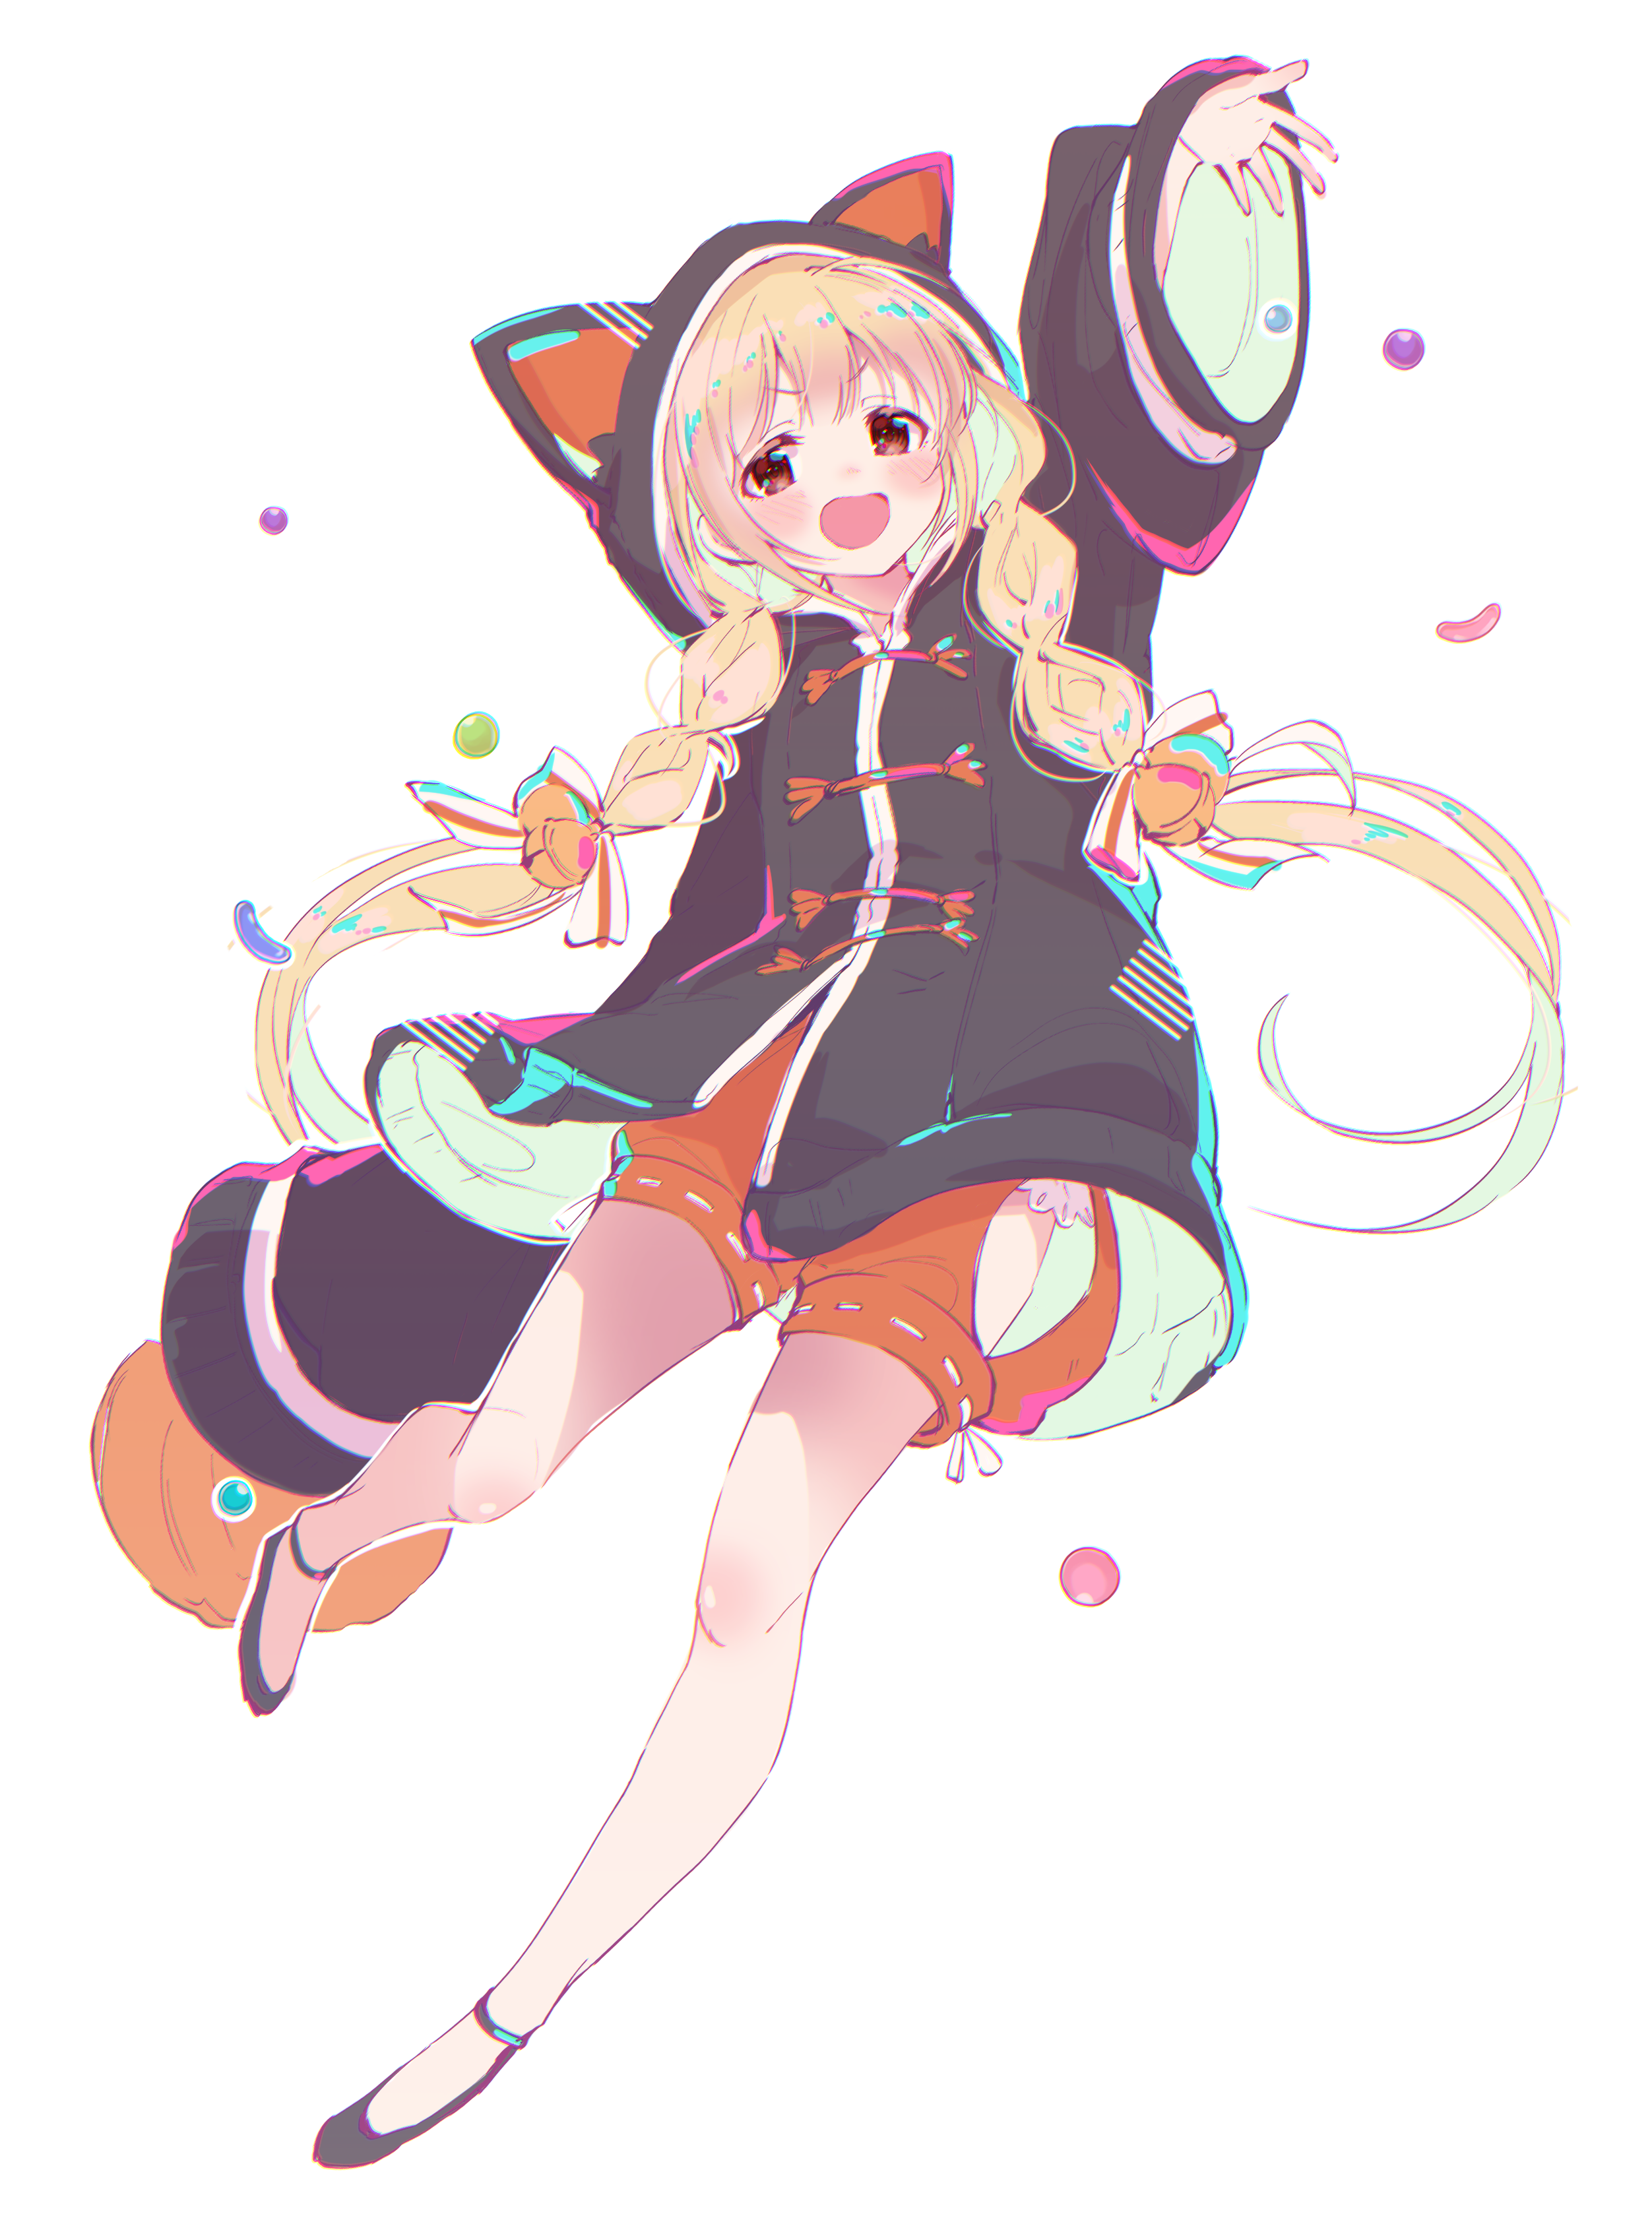
\includegraphics[width=10.5cm]{images/idolm.png}};
				\draw[anchor=north east, inner sep=0pt] (18.65cm,-2.75cm) node
				[black, 
					ultra thick,
					%fill=tsorange!10,
					fill opacity=.75,
					inner sep=10pt]
				(0,0)
				{\parbox[t][20cm][t]{3cm}{\begin{centering}
							\mutou{{\fontsize{50}{40}\selectfont \rotatebox{3}{\textcolor[HTML]{9A99D3}{数}}\\\rotatebox{2}{\textcolor[HTML]{FDD100}{学}}\\\rotatebox{357}{\textcolor[HTML]{F29A85}{\hspace{0.1cm}题}}\\\rotatebox{0}{\textcolor[HTML]{A2DC25}{\hspace{0.1cm}练}}\\\rotatebox{1}{\textcolor[HTML]{FDD100}{习}}\\[0.25em]\rotatebox{2}{\textcolor[HTML]{66CDF8}{\hspace{0.5cm}帐}}
							}} \vspace{0.2cm}
							\par\hspace{0cm}\begin{tcolorbox}[enhanced,top=1mm,bottom=1mm,width=6em,
								right=1mm,left=1mm,arc=0.5em,
								opacityback=1,
								colframe=tsorange!90,coltext=tsorange!90]\centering\Huge{\youyuan{草\hspace{0.5mm}稿}}\ \end{tcolorbox}
						\end{centering}
					}
				};

				\draw[anchor=north east, inner sep=0pt] (17.25cm,-2.85cm) node
				[black,
					ultra thick,
					%fill=,
					fill opacity=0.75,
					inner sep=10pt]
				(0,0)
				{\parbox[t][20cm][t]{2cm}{\begin{centering}
							\Huge{\bfseries{\textcolor{brown}{\rotatebox{270}{BY\ TAKENOKO1997 ON 2021.01.20}}}}
						\end{centering}
					}
				};

				\draw[anchor=south east, inner sep=0pt] (18.5cm,-27.5cm) node
				[black,
					ultra thick,
					%fill=,
					fill opacity=0.9,
					inner sep=10pt]
				(0,0)
				{\begin{tcolorbox}
					[enhanced jigsaw,breakable,pad at break*=1mm,
					opacityback=0,colframe=brown,width=7cm,top=0mm,left=0mm]
					\textcolor{brown}{
						\begin{enumerate}
							\item 由于很多题目没有答案,所以解答可以保证过程正确,不保证结果正确。\textbf{切记自己计算}。
							\item 若发现错误,可请告知,我来修改。
							\item 楷体部分和旁注介绍了一些注意点和补充背景,可选择性读。
							\item 本文地址:\href{https://github.com/359950539/KoukouFunctionExercises}{GitHub}\ \ \href{https://pantsu.ink}{Blog}
						\end{enumerate}
					}
					\end{tcolorbox}
				};
				%\node[anchor=north west,inner sep=0pt] at
			\end{tikzpicture}
		};%
	  \end{tikzpicture}
\end{titlepage}
%----------------------------------------------------------------------------------------
%	BOOK INFORMATION
%----------------------------------------------------------------------------------------

% \titlehead{The \texttt{kaobook} class}
% \subject{Use this document as a template}

% \title[Example and documentation of the {\normalfont\texttt{kaobook}} class]{Example and documentation \\ of the {\normalfont\texttt{kaobook}} class}
% \subtitle{Customise this page according to your needs}

% \author[Federico Marotta]{Federico Marotta \thanks{A \LaTeX\ lover}}

% \date{\today}

% \publishers{An Awesome Publisher}

%----------------------------------------------------------------------------------------

\frontmatter % Denotes the start of the pre-document content, uses roman numerals

%----------------------------------------------------------------------------------------
%	OPENING PAGE
%----------------------------------------------------------------------------------------

%\makeatletter
%\extratitle{
%	% In the title page, the title is vspaced by 9.5\baselineskip
%	\vspace*{9\baselineskip}
%	\vspace*{\parskip}
%	\begin{center}
%		% In the title page, \huge is set after the komafont for title
%		\usekomafont{title}\huge\@title
%	\end{center}
%}
%\makeatother

%----------------------------------------------------------------------------------------
%	COPYRIGHT PAGE
%----------------------------------------------------------------------------------------

% \makeatletter
% \uppertitleback{\@titlehead} % Header

% \lowertitleback{
% 	\textbf{Disclaimer}\\
% 	这是什么东西なにこれYou can edit this page to suit your needs. For instance, here we have a no copyright statement, a colophon and some other information. This page is based on the corresponding page of Ken Arroyo Ohori's thesis, with minimal changes.
	
% 	\medskip
	
% 	\textbf{No copyright}\\
% 	\cczero\ This book is released into the public domain using the CC0 code. To the extent possible under law, I waive all copyright and related or neighbouring rights to this work.
	
% 	To view a copy of the CC0 code, visit: \\\url{http://creativecommons.org/publicdomain/zero/1.0/}
	
% 	\medskip
	
% 	\textbf{Colophon} \\
% 	This document was typeset with the help of \href{https://sourceforge.net/projects/koma-script/}{\KOMAScript} and \href{https://www.latex-project.org/}{\LaTeX} using the \href{https://github.com/fmarotta/kaobook/}{kaobook} class.
	
% 	The source code of this book is available at:\\\url{https://github.com/fmarotta/kaobook}
	
% 	(You are welcome to contribute!)
	
% 	\medskip
	
% 	\textbf{Publisher} \\
% 	First printed in May 2019 by \@publishers
% }
% \makeatother

%----------------------------------------------------------------------------------------
%	DEDICATION
%----------------------------------------------------------------------------------------

% \dedication{
% 	The harmony of the world is made manifest in Form and Number, and the heart and soul and all the poetry of Natural Philosophy are embodied in the concept of mathematical beauty.\\
% 	\flushright -- D'Arcy Wentworth Thompson
% }

%----------------------------------------------------------------------------------------
%	OUTPUT TITLE PAGE AND PREVIOUS
%----------------------------------------------------------------------------------------

% Note that \maketitle outputs the pages before here

% If twoside=false, \uppertitleback and \lowertitleback are not printed
% To overcome this issue, we set twoside=semi just before printing the title pages, and set it back to false just after the title pages
% \KOMAoptions{twoside=semi}
% \maketitle
% \KOMAoptions{twoside=false}

%----------------------------------------------------------------------------------------
%	PREFACE
%----------------------------------------------------------------------------------------

% \chapter*{Preface}
\addcontentsline{toc}{chapter}{Preface} % Add the preface to the table of contents as a chapter

I am of the opinion that every \LaTeX\xspace geek, at least once during 
his life, feels the need to create his or her own class: this is what 
happened to me and here is the result, which, however, should be seen as 
a work still in progress. Actually, this class is not completely 
original, but it is a blend of all the best ideas that I have found in a 
number of guides, tutorials, blogs and tex.stackexchange.com posts. In 
particular, the main ideas come from two sources:

\begin{itemize}
	\item \href{https://3d.bk.tudelft.nl/ken/en/}{Ken Arroyo Ohori}'s 
	\href{https://3d.bk.tudelft.nl/ken/en/nl/ken/en/2016/04/17/a-1.5-column-layout-in-latex.html}{Doctoral 
	Thesis}, which served, with the author's permission, as a backbone 
	for the implementation of this class;
	\item The 
		\href{https://github.com/Tufte-LaTeX/tufte-latex}{Tufte-Latex 
			Class}, which was a model for the style.
\end{itemize}

The first chapter of this book is introductory and covers the most
essential features of the class. Next, there is a bunch of chapters 
devoted to all the commands and environments that you may use in writing 
a book; in particular, it will be explained how to add notes, figures 
and tables, and references. The second part deals with the page layout 
and design, as well as additional features like coloured boxes and 
theorem environments.

I started writing this class as an experiment, and as such it should be 
regarded. Since it has always been intended for my personal use, it may
not be perfect but I find it quite satisfactory for the use I want to 
make of it. I share this work in the hope that someone might find here 
the inspiration for writing his or her own class.

\begin{flushright}
	\textit{Federico Marotta}
\end{flushright}

% \index{preface}

%----------------------------------------------------------------------------------------
%	TABLE OF CONTENTS & LIST OF FIGURES/TABLES
%----------------------------------------------------------------------------------------

\begingroup % Local scope for the following commands

% Define the style for the TOC, LOF, and LOT
%\setstretch{1} % Uncomment to modify line spacing in the ToC
%\hypersetup{linkcolor=blue} % Uncomment to set the colour of links in the ToC
\setlength{\textheight}{230\hscale} % Manually adjust the height of the ToC pages

% Turn on compatibility mode for the etoc package
\etocstandarddisplaystyle % "toc display" as if etoc was not loaded
\etocstandardlines % "toc lines as if etoc was not loaded

\tableofcontents % Output the table of contents

\listoffigures % Output the list of figures

% Comment both of the following lines to have the LOF and the LOT on different pages
\let\cleardoublepage\bigskip
\let\clearpage\bigskip

\listoftables % Output the list of tables

\endgroup

%----------------------------------------------------------------------------------------
%	MAIN BODY
%----------------------------------------------------------------------------------------

\mainmatter % Denotes the start of the main document content, resets page numbering and uses arabic numbers
\setchapterstyle{kao} % Choose the default chapter heading style

\setchapterpreamble[u]{\margintoc}
\chapter{基础题目}
\labch{Basic}
\section{基础知识}
符号:
\begin{description}
	\item[$f^n(x)$] 表示$f$的$n$次复合,$\underbrace{f(f(\cdots f(x)))}_{n\text{层}}$。特别地,$f^0(x)=x$。 
	\item[$\binom{m}{n}$] 表示$m$中取$n$的组合数,$\binom{m}{n}=C_m^n=\dfrac{m!}{n!(m-n)!}$ 。
\end{description}
常见函数的导数:\\
\begin{center}
	\begin{tabular}{lll}
		\hline
		函数&导函数&定义域\\
		\hline
		$ax^n$&$anx^{n-1}$&$x\in\mathbb{R},n\neq 0$\\
		$a^x$&$a^x\ln a$&$x \in \mathbb{R},a\neq 0$\\
		$e^x$&$e^x$&$x \in \mathbb{R}$\\
		$\ln x$&$\dfrac{1}{x}$&$x \in (0,+\infty)$\\
		$\log_a{x}$&$\dfrac{1}{x\ln a}$&$x,a \in (0,+\infty)$\\
		$\sin x$&$\cos x$&$x\in \mathbb{R}$\\
		$\cos x$&$-\sin x$&$x\in \mathbb{R}$\\
		$\tan x$&$\dfrac{1}{\cos^2 x}$&$x \neq \dfrac{(2n+1)\pi}{2}, n \in \mathbb{Z}$\\[0.5em]
		\hline
	\end{tabular} 
\end{center}
复合函数的导数:\par\vspace{1em}
\begin{tabular}{ccccc}
	\hline\\[-1em]
	函数&$f(g(x))$&$f(x)+g(x)$&$f(x)g(x)$&$\dfrac{f(x)}{g(x)}$\\[1em]
	\hline\\[-1em]
	导函数&$g'(x)f'(g(x))$&$f'(x)+g'(x)$&$f'(x)g(x)+f(x)g'(x)$&$\dfrac{f'(x)g(x)-f(x)g'(x)}{[g(x)]^2}$\\[1em]
	\hline
\end{tabular}\par\vspace{1em}
函数积的多次导数(莱布尼兹公式):
$$\left[f(x)g(x)\right]^{(n)}=\sum_{k=0}^n \binom{n}{k} f^{(k)}(x)g^{(n-k)}(x)=C_n^0f(x)g^{(n)}(x)+C_n^1f'(x)g^{(n-1)}(x)+\cdots+C_n^nf^{(n)}(x)g(x)$$
\section{函数的概念}

\begin{que}
	已知函数$f(x)$定义域为$\left[-\dfrac{1}{2},\dfrac{3}{2}\right]$,$a>0$,求函数$g(x)=f(ax)+f\left(\dfrac{x}{a}\right)$的定义域。
\end{que}
\sol 过程略。\begin{enumerate}
	\item 当$a\geqslant 1$时,所求定义域$\res{\left[-\dfrac{1}{2a},\dfrac{3}{2a}\right]}$;
	\item 当$0<a<1$时,所求定义域$\res{\left[-\dfrac{a}{2},\dfrac{3a}{2}\right]}$。\hfill\tg{定义域}\easy
\end{enumerate} 

\begin{que}
	求下面函数的值域:(1)$y=\dfrac{2\sin x-1}{2\sin x+1}$\ (2)$y=\dfrac{e^x-e^{-x}}{e^x+e^{-x}}$\ \\[0.5em](3)$y=(x+1)(x+2)(x+3)(x+4),x\in[-3,3]$
\end{que}
\sol \begin{enumerate}
	\item \blue{(方法一)}\sidenote{但凡有单值反函数,那末反函数的定义域即为函数的值域,反函数的值域即为函数的定义域。}反解$\sin x$得$\sin x= \dfrac{1+y}{2(1-y)}$,由$\sin x\in[-1,1]$知,严格地,$$|\sin x|=\left|\dfrac{1+y}{2(1-y)}\right|\leqslant 1\ \Leftrightarrow\ (1+y)^2\leqslant 4(1-y)^2\ \Leftrightarrow\ \res{y\in\left(-\infty,\dfrac{1}{3}\right]\cup[3,+\infty)}$$
	\blue{(方法二)}记$t=\sin x\in[-1,1]$,则$$y=\dfrac{2t-1}{2t+1}=1-\dfrac{2}{2t+1}\res{\in\left(-\infty,\dfrac{1}{3}\right]\cup[3,+\infty)}$$
	\item 两种方法同上,此处不赘述。$\res{y\in(-1,1)}$。
	\item 对称展开得$y=(x^2+5x+4)(x^2+5x+6)=(t+4)(t+6)=(t+5)^2-1$,其中$t=x^2+5x\in\left[-\dfrac{25}{4},24\right]$,结合二次函数图像可知$y=(t+5)^2-1\in\res{[-1,840]}$。\par\hfill\tg{反函数\ 值域}\easy
\end{enumerate}

\begin{que}
	求下列函数的值域:(1)$f(x)=-\dfrac{x^2-x+2}{x^2+2}$\ (2)$f(x)=x-\sqrt{1-x^2}$
\end{que}
\sol \begin{enumerate}
	\item \blue{(方法一)}$f(x)=-\dfrac{x^2-x+2}{x^2+2}=\dfrac{1}{\dfrac{2}{x}+x}-1$,分母是对勾函数\sidenote{当我们上下同除$x$时,事实上假定了$x\neq 0$,因此计算后须对$x=0$时的取值进行补充。这样做是无妨的,原因有二,一是$f(x)$是连续的,二是我们完全可以补充$\dfrac{1}{\infty}=0$。},其值域为$\dfrac{2}{x}+x\in(-\infty,-2\sqrt{2})\cup(2\sqrt{2},+\infty)$,另外$f(-1)=0$,因此得值域$\res{\left[-1-\dfrac{\sqrt{2}}{4},-1+\dfrac{\sqrt{2}}{4}\right]}$。\par
	\blue{(方法二)}	注意到分母不为$0$。记$f(x)=y$,则原式$\ \Leftrightarrow\ (y+1)x^2-x+(2y+2)=0$,视之为关于$x\in\mathbb{R}$的二次函数\sidenote{形如$f(x)=\dfrac{a_1x^2+b_1x+c_1}{a_2x^2+b_2x+c_2}$和$f(x)=ax+b+c\sqrt{dx^2+ex+f}$的函数式均可尝试用判别式的方法求值域。},那末$$\Delta=1-4(y+1)(2y+2)\geqslant 0\ \Leftrightarrow\ y\in\res{\left[-1-\dfrac{\sqrt{2}}{4},-1+\dfrac{\sqrt{2}}{4}\right]}$$
	\begin{marginfigure}
		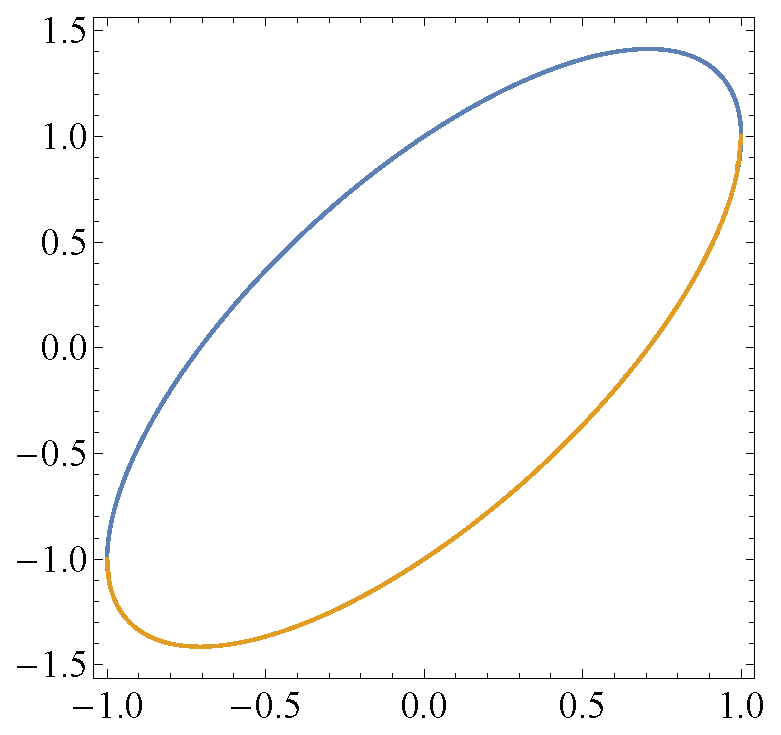
\includegraphics{Figure-3.eps}
		\caption{$2x^2-2x y+y^2=1$的图像。橙色部分即为(2)中$f(x)$的图像。}
	\end{marginfigure}
	\item \blue{(方法一)}设$x=\sin t\in[-1,1]$\sidenote{为何设三角函数对于类似形式的函数可以起到等价化简的作用?因为这原本就是二次圆锥曲线的变形,本题(2)中的函数即是旋转的椭圆。},则$f(x)=\sin t-|\cos t|\in\res{[-\sqrt{2},1]}$。\par
	\blue{(方法二)}易知$f(x)$在$[0,1]$上有$f(x)\geqslant f(-x)$且单调增,$x\in[-1,1]$,因此严格地$f(x)\leqslant f(1)=1$。又$$(y-x)^2=1-x^2\ \Leftrightarrow\ 2x^2-2xy+y^2-1=0\ \\\Rightarrow\ \Delta=8-4y^2\geqslant 0\ \Leftrightarrow\ f(x)=y\in[-\sqrt{2},\sqrt{2}]$$
	注意到$f\left(-\dfrac{\sqrt{2}}{2}\right)=-\sqrt{2}$,$f(x)$连续\sidenote{求最值和求值域是不同的,函数不一定能取到最大值和最小值之间的值,然而函数必然可以取到值域中的所有值。},故值域$\res{f(x)\in[-\sqrt{2},1]}$。
\end{enumerate}\par\hfill\tg{判别式\ 值域}\easy

\begin{que}
	\begin{enumerate}
		\item 已知函数$f(x)=\log_a\left(x+\dfrac{a}{x}-4\right)$的定义域为$\mathbb{R}$,其中$a>0$,$a\neq 1$,求实数$a$的取值范围。
		\item 已知函数$f(x)=\log_3\dfrac{mx^2+8x+n}{x^2+1}$的定义域为$\mathbb{R}$,值域为$[0,2]$,求$m,n$的值。
		\item 设函数$f(x)=\log_3\dfrac{bx^2+ax+b}{x^2+x+1}$,已知$a>b$,函数的值域为$(-\infty,0]$,求$a$的取值范围。
	\end{enumerate}
\end{que}
\sol \begin{enumerate}
	\item 值域为$\mathbb{R}$意味着$x+\dfrac{a}{x}-4$值域包含$\mathbb{R}^+$,又$a>0$,故这是一个对勾函数,其最小值为$x+\dfrac{a}{x}-4\geqslant 2\sqrt{x\cdot\dfrac{a}{x}}-4=2\sqrt{a}-4$,那末只需使$2\sqrt{a}-4\leqslant 0\Rightarrow\res{a\in(0,1)\cup(1,4]}$。
	\item 由于$f(x)$定义域为$\mathbb{R}$,故$\forall x\in \mathbb{R}$,恒有$$\dfrac{mx^2+8x+n}{\underbrace{x^2+1}_{>0}}>0\ \Leftrightarrow\ \text{\footnotesize 分母}\Delta=64-4mn<0,m>0$$
	又根据值域有\sidenote{此过程中暗含使用了$x\in\mathbb{R}$这一条件,因此我们可以毫无顾虑的使用判别式计算。同时闭区间端点对应的是边界条件,放在不等式上意味着「取等」。}$$\begin{aligned}\dfrac{mx^2+8x+n}{x^2+1}=k\in[1,9]\ &\Leftrightarrow\ k^2-(m+n)k+mn-16\leqslant 0,\forall k\in[1,9]\ \\
		&\Rightarrow\ m+n=10,mn-16=9\ \Rightarrow\ \res{m=n=5}\end{aligned}$$
	\item 由题条件\sidenote{本小题对定义域没有说明和限制,但并不意味着定义域为$\mathbb{R}$。},$$\dfrac{bx^2+ax+b}{\underbrace{x^2+x+1}_{>0}}=k\in(0,1]\ \Rightarrow\ (b-k)x^2+(a-k)x+(b-k)=0$$当$k\in(0,1]$时恒有解,$k>1$时无解。因此
	$$\begin{aligned}&\quad\ \forall k\in(0,1],\ \Delta=(a-k)^2-4(b-k)^2\geqslant 0,\text{且}k=1\text{处取等,下同}\\
	&\Leftrightarrow\ \forall k\in(0,1],\ \left(k-\dfrac{a+2b}{3}\right)(k-(2b-a))\geqslant 0\end{aligned}$$
	由于$a>b$,故$\dfrac{a+2b}{3}>2b-a$,$$\left\{\begin{aligned}&\dfrac{a+2b}{3}=1\\& 2b-a\leqslant 0\end{aligned}\right.\ \Rightarrow\ \res{a\geqslant\dfrac{3}{2}}$$
\end{enumerate}\par\hfill\tg{复合函数}\normal

\begin{que}
	已知$f(x)=\sqrt{4-x^2}$在闭区间$M$上的反函数是其本身,求$M$的取值集合。
\end{que}
\sol 显然$f(x)$函数图像为半径为$2$,圆心在原点的圆的上半部分。结合函数与其反函数图像的几何关系\sidenote{函数与其反函数关于直线$x=y$镜像对称。},可知$M$的取值集合为$\res{M\in\left\{[2\sin\theta,2\cos\theta]:\theta\in\left[0,\dfrac{\pi}{4}\right]\right\}}$。\par\hfill\tg{反函数\ 圆}\easy

\begin{que}
	设定义域为$\mathbb{R}$的函数$f(x),g(x)$均有反函数,且函数$f(x-1)$和$g^{-1}(x-2)$的图像关于直线$y=x$对称,若$g(5)=2021$,求$f(4)$的值。
\end{que}
\sol 由题意$(5,f(4))$与$(f(4),g^{-1}(f(4)-2))$关于$y=x$对称,故$g^{-1}(f(4)-2)=5$,由于$g(x)$有反函数,故$g$为双射\sidenote{\textbf{双射:}若关于映射$f:A\rightarrow B$有以下两特点,则称映射$f$为双射,也即「一一映射」:
\begin{enumerate}
	\item $\forall y\in B,\exists x\in A,\text{\ s.t.\ }f(x)=y$(满射)
	\item 若$x_1\in A,x_2\in A,f(x_1)=f(x_2)$,则必有$x_1=x_2$(单设)
\end{enumerate}若一个函数有反函数,即一个映射有它的逆,那末它必是双射。},因此$f(4)-2=2021\Rightarrow\res{f(4)=2023}$。\par\hfill\tg{反函数}\easy

\begin{que}
	设函数$f:\mathbb{R}\rightarrow\mathbb{R}$满足$f(0)=1$,且$\forall x,y\in\mathbb{R}$都有$f(xy+1)=f(x)f(y)-f(y)-x+2$,求$f(x)$的表达式。
\end{que}
\sol 令$x=y=0$,可得$f(1)=2$;令$y=0$,可得$f(1)=2=f(x)f(0)-f(0)-x+2=f(x)-x+1\Rightarrow\res{f(x)=x+1}$。\par\hfill\tg{抽象函数}\easy

\begin{que}
	设定义在整数集上的函数$f$满足$f(n)=\left\{ \begin{aligned}
		&n+5&n<2000\\&f(f(n-8))&n\geqslant 2000
	\end{aligned}\right.$,求$f(4096)$。
\end{que}
\sol 我们使用符号$f^k(x)$表记$\overbrace{f(f(f(\cdots f(x))))}^{k\text{次}f\text{复合}}$,那末
$$\begin{aligned}
	&\quad\ f(4096)=f^2(4088)=\cdots=f^{263}(2000)=f^{264}(1992)\\
	&=f^{262}(2002)=f^{263}(1994)=f^{261}(2004)=f^{262}(1996)=f^{261}(2001)\\
	&=f^{262}(1993)=f^{260}(2003)=f^{261}(1995)=f^{260}(2000)\end{aligned}
	$$
	这里我们得到了第一个周期$f^{263}(2000)=f^{260}(2000)$,因此可知$\forall n\geqslant 2000,k\in\mathbb{Z}$,$f^{k+3}(n)=f^k(n)$,因此$f(4096)=f^{261}(2004)=f^0(2004)=\res{2004}$。
	事实上可以求出,$\forall n\geqslant 2000$,$f(n)=2002+(n+1)\%3$,其中「\%」为取余符号。\par\hfill\tg{抽象函数}\normal

\begin{que}
	已知函数$f(x)=\dfrac{2x^2+bx+c}{x^2+1}$的值域为$[1,3]$,其中$b<0$。
	\begin{enumerate}
		\item 求实数$b,c$的值。
		\item 判断$F(x)=\lg f(x)$在$[-1,1]$上的单调性,并给出证明。
		\item 若$t\in\mathbb{R}$,求证:$\lg\dfrac{7}{5}\leqslant F\left(\left|t-\dfrac{1}{6}\right|-\left|t+\dfrac{1}{6}\right|\right)\leqslant\lg\dfrac{13}{5}$。
	\end{enumerate}
\end{que}
\sol \begin{enumerate}
	\item 记$y=f(x)$,定义域$x\neq\pm 1$。整理得$(y-2)x^2-bx+(y-c)=0\ \Rightarrow\ \Delta=b^2-4(y-2)(y-c)\geqslant 0$,由于$y=f(x)$的值域为$[1,3]$,因此$\Delta|_{y=1}=\Delta|_{y=3}=0\ \Rightarrow\ \res{b=-2,c=2}$。
	\item 由于$\lg x$是增函数,因此其增减性与$f(x)$一致。$f'(x)=\dfrac{2(x^2-1)}{(x^2+1)^2}<0$,因此$F(x)=\lg x$在$[-1,1]$上单调减。
	\item 根据$F(x)$的递减性,只需找到$h(t)=\left|t-\dfrac{1}{6}\right|-\left|t+\dfrac{1}{6}\right|$的值域。首先$h(t)$是连续的,$$h(t)\leqslant\left|\left(t-\dfrac{1}{6}\right)-\left(t+\dfrac{1}{6}\right)\right|=\dfrac{1}{3}\qquad\footnotesize{\text{当}t=-\dfrac{1}{6}\text{时取等}}$$由于$h(t)$是奇函数,因此其最小值为$\min h(t)=-\max h(t)=-\dfrac{1}{3}$。综上,$${\lg\dfrac{7}{5}}=F\left(\dfrac{1}{3}\right)\leqslant F(h(t))\leqslant F\left(-\dfrac{1}{3}\right)={\lg\dfrac{13}{5}}$$
\end{enumerate}\par\hfill\tg{绝对值不等式\ 值域}\easy
%%%%%%%%%%%%%%%%%%%抽象函数%%%%%%%%%%%%%%%%%%%%%%
\section{抽象函数}
抽象函数相关题目在试题中出现的不多,然而由于它需要对函数概念有较深的理解,并有一定的函数分析能力,因此不乏不错的习题。抽象函数有一些常出现的模型,列举如下:
\begin{center}
	\begin{tabular}{lll}
		\hline
		模型&方程式&备注\\
		\hline
		一次函数模型&$f(x+y)=f(x)+f(y)$&\\
		幂函数模型&$f(xy)=f(x)f(y)$&\\
		指数函数模型&$f(x+y)=f(x)f(y)$&\\
		对数函数模型&$f(xy)=f(x)+f(y)$&\\[0.25em]
		余切函数模型&$f(x+y)=\dfrac{f(x)-f(y)}{1-f(x)f(y)}$&$\cot x=\dfrac{1}{\tan x}$\\[1em]
		正切函数模型&$f(x+y)=\dfrac{f(x)+f(y)}{1-f(x)f(y)}$&\\[1em]
		双曲正切函数模型&$f(x+y)=\dfrac{f(x)+f(y)}{1+f(x)f(y)}$&$\tanh x=\dfrac{e^x-e^{-x}}{e^x+e^{-x}}$\\[1em]
		\hline
	\end{tabular} 
\end{center}
函数的性质:
\begin{description}
	\item[奇偶性] $\forall x\in D$,若$-x\in D$且$f(x)=-f(-x)$,称函数为奇函数;$\forall x\in D$,若$-x\in D$且$f(x)=f(-x)$,称函数为偶函数。
	\item[有界性] 若$\exists M<\infty$,使得$\forall x\in S\subset D$,$f(x)<M$,称$f(x)$在$S$上有上界$M$;若$\exists N<\infty$,使得$\forall x\in S\subset D$,$f(x)>N$,称$f(x)$在$S$上有下界$N$;若$f(x)$在$S$上有上下界,称$f(x)$在$S$上有界。
	\item[单调性] 若$\forall x_1,x_2\in S\subset D,x_1>x_2$,恒有$f(x_1)-f(x_2)\geqslant 0$,称$f(x)$在$S$上单调递增,若式中等号无法取得,称$f(x)$在$S$上严格单调递增;若$\forall x_1,x_2\in S\subset D,x_1>x_2$,恒有$f(x_1)-f(x_2)\leqslant 0$,称$f(x)$在$S$上单调递减,若式中等号无法取得,称$f(x)$在$S$上严格单调递减。
	\item[连续性] 固定$x_0\in D$,若$\forall\varepsilon>0$,$\exists \delta(\varepsilon)>0$,s.t\ $\forall x\in(x_0,x_0+\delta(\varepsilon))$,$|f(x_0)-f(x)|<\varepsilon$,称$f(x)$在$x=x_0$处右连续;固定$x_0\in D$,若$\forall\varepsilon>0$,$\exists \delta(\varepsilon)>0$,s.t\ $\forall x\in(x_0-\delta(\varepsilon),x_0)$,$|f(x_0)-f(x)|<\varepsilon$,称$f(x)$在$x=x_0$处左连续;若$f(x)$在$x=x_0$处左连续且右连续,称$f(x)$在$x=x_0$处连续。
	\item[可导性] 固定$x_0\in D$,若$\exists a<\infty$,$\forall\varepsilon>0$,$\exists \delta(\varepsilon)>0$,s.t\ $\forall x\in(x_0,x_0+\delta(\varepsilon))$,$\left|\dfrac{f(x)-f(x_0)}{x-x_0}-a\right|<\varepsilon$,称$f(x)$在$x=x_0$处右导数存在且为$a$;固定$x_0\in D$,若$\exists b<\infty$,$\forall\varepsilon>0$,$\exists \delta(\varepsilon)>0$,s.t\ $\forall x\in(x_0-\delta(\varepsilon),x_0)$,$\left|\dfrac{f(x_0)-f(x)}{x_0-x}-b\right|<\varepsilon$,称$f(x)$在$x=x_0$处左导数存在且为$b$;若$f(x)$在$x=x_0$处左右导数都存在且$a=b=A$,称$f(x)$在$x=x_0$处可导且导数为$A$。$x$到$f(x)$在$x$处导数的映射称为$f(x)$的导函数。可导必定连续。连续不一定可导。\sidenote{连续性和可导性可在定义极限后改用极限语言叙述,可复习教材定积分一章。}
\end{description}
\begin{que}
	\begin{enumerate}
		\item 若函数$f(x)$满足$\forall x\neq 0$,$f(x)+2f\left(\dfrac{1}{x}\right)=3x$,求$f(x)$的显性表达式。
		\item 若函数$f(x)$满足$\forall x\neq 0$,$f(x)+f\left(\dfrac{x-1}{x}\right)=1+x$,求$f(x)$的显性表达式。
		\item 若函数$f(x)$满足$\forall x\neq 0$,$$f\left(\dfrac{x-1}{x+1}\right)+f\left(-\dfrac{1}{x}\right)+f\left(\dfrac{1+x}{1-x}\right)=\cos x$$求$f(x)$的显性表达式。
	\end{enumerate}
\end{que}
\sol \begin{enumerate}
	\item 令$x=\dfrac{1}{x}$(此处为赋值),得$2f(x)+f\left(\dfrac{1}{x}\right)=\dfrac{3}{x}$,与题中条件联立得$\res{f(x)=\dfrac{2}{x}-x}$。
	\item 记$g(x)=\dfrac{x-1}{x}$,我们注意到这样一个事实\sidenote{这一事实启示了我们,若有一个数列$\{a_n\}$,其递推式为$a_{n+1}=1-\dfrac{1}{a_n}$,那末$\{a_n\}$为周期数列。这里结合数列知识可以展开很多,不过与章节内容不符,故不赘述。}:$\forall n\in\mathbb{N}$,$g^{n+3}(x)=\underbrace{g(g(\cdots g(x)))}_{n+3\text{层复合}}=g^n(x)$,因此若记\sidenote{以下两种记号应当作区分:$f^n(x)$表示$\underbrace{f(f(\cdots f(x)))}_{n\text{层复合}}$;$[f(x)]^n$表示$\underbrace{f(x)f(x)\cdots f(x)}_{n\text{个}f(x)\text{乘积}}$。只有在不造成混淆的情况下,可用第一种记号表示函数值的乘方。事实上,函数的复合被视为映射的乘积,这就是第一种记号的来源。}$a=f(x)=f(g^0(x)),b=f(g(x)),c=f(g^2(x))$,赋值$x=x,x=g(x),x=g^2(x)$,可得三个等式:
	$$\left\{\begin{aligned}
		&a+b=f(x)+f(g(x))=1+x\\
		&b+c=f(g(x))+f(g^2(x))=1+g(x)\\
		&c+a=f(g^2(x))+f(g^3(x))=f(g^2(x))+f(x)=1+g^2(x)
	\end{aligned}\right.$$
	解之得$$a=f(x)=\dfrac{1}{2}\left[(1+x)-(1+g(x))+1+g^2(x)\right]=\res{\dfrac{x^3-x^2-1}{2x(x-1)}}$$
	\item 记$g(x)=\dfrac{1-x}{1+x}$,注意到这样一个事实:$g^2(x)=-\dfrac{1}{x}$,$g^3(x)=\dfrac{1+x}{1-x}$,$g^4(x)=x=g^0(x)$,因此原式可改写为:$f(g(x))+f(g^2(x))+f(g^3(x))=\cos x$,赋值$x=x,x=g(x),x=g^2(x)$,可得四个等式:
	$$\left\{\begin{aligned}
		&f(g(x))+f(g^2(x))+f(g^3(x))=\cos x\\
		&f(g^2(x))+f(g^3(x))+f(x)=\cos g(x)\\
		&f(g^3(x))+f(x)+f(g(x))=\cos g^2(x)\\
		&f(x)+f(g(x))+f(g^2(x))=\cos g^3(x)
	\end{aligned}\right.$$解之得\sidenote{函数$$f(x)=\dfrac{x\cos\dfrac{2\pi}{m}-\sin\dfrac{2\pi}{m}}{x\sin\dfrac{2\pi}{m}+\cos\dfrac{2\pi}{m}}$$满足$f^m(x)=x$,2,3两小题出题背景即是此式。此式的背景为旋转变换,可自行查阅旋转变换相关的拓展知识。}$$\begin{aligned}f(x)&=\dfrac{1}{3}\left[-2\cos x+\cos g(x)+\cos g^2(x)+\cos g^3(x)\right]\\&=\res{\dfrac{1}{3}\left[-2\cos x+\cos\dfrac{1-x}{1+x}+\cos\dfrac{1}{x}+\cos\dfrac{1+x}{1-x}\right]}\end{aligned}$$
\end{enumerate}
\par\hfill\tg{抽象函数}\normal

\begin{que}
	\begin{enumerate}
		\item 求所有的函数$f:\mathbb{R}\rightarrow\mathbb{R}$,使得$\forall x,y\in\mathbb{R}$,下式恒成立:$$(x-y)f(x+y)-(x+y)f(x-y)=4xy(x^2-y^2)$$
		\item 求所有的函数$f:\mathbb{R}\rightarrow\mathbb{R}$,使得$\forall x,y\in\mathbb{R}$,下式恒成立:$$f(f(x)+y)=2x+f(f(f(y))-x)$$
		\item 求所有的函数$f:\mathbb{R}\rightarrow\mathbb{R}$,使得$\forall x,y\in\mathbb{R}$,下式恒成立:$$f(x+y)+f(x-y)=2f(x)\cos y$$
	\end{enumerate}
\end{que}
\sol \begin{enumerate}
	\item \sidenote{本题背景为图像的旋转变换$(x,y)\mapsto (x\cos \theta -y\sin\theta ,\ x\sin\theta +y\cos\theta )$,以及线性组合。}设$u=x+y$,$v=x-y$,原式可化为$$vf(u)-uf(v)=(u^2-v^2)uv\ \Leftrightarrow\ \dfrac{f(u)}{u}-\dfrac{f(v)}{v}=u^2-v^2$$显然$f(x)=x^3$为一特解,我们需要找到所有解,即通解。假设有另一解$f(x)=x^3+xg(x)$,$g(x)$为同定义域的未知函数,代入原式得$$\forall u,v\in\mathbb{R},\ g(u)-g(v)=0\ \Leftrightarrow\ g(x)\equiv C$$其中$C$为一实常数。因此通解为$\res{f(x)=x^3+C,\ C\in\mathbb{R}}$。
	\item 我们先求$f(0)$。令$x=y=0$,得$f^2(0)=f^3(0)\Rightarrow\forall n\geqslant 2,f^n(0)=f^2(0)$;令$y=0,x=f^2(0)$,得$f^4(0)=f^2(0)=2f^2(0)+f(0)\Rightarrow -f(0)=f^2(0)$;令$x=0,y=-f(0)$,得$$f(0)=f(f^2(-f(0)))=f^5(0)=-f(0)\ \Rightarrow\ f(0)=0$$
	令$y=0$,得$f^2(x)=2x+f(-x)$;令$y=x,x=0$,得$f(x)=f^3(x)$;令$y=-f(x)$,得$$f(0)=0=2x+f(f^2(-f(x))-x)$$令$x=f(x),y=0$,得$$f^3(x)=2f(x)+f(-f(x))\ \Rightarrow\ f(-f(x))=-f(x)$$赋值$x=f(x)$之后,似乎可以认为$f(x)=x$了,不过因为$f:\mathbb{R}\rightarrow \mathbb{R}$,我们须得\sidenote{在做变量代换时,切记观察定义域是否有变动。}确认$f(x)$可遍历$\mathbb{R}$。回代之得$\forall x\in\mathbb{R}$,$$0=2x+f(f(f(-f(x)))-x)=2x+f(-f(x)-x)$$故$f(x)$可遍历$\mathbb{R}$。因此可以确认只有$\res{f(x)=x}$符合题意。
	\item \sidenote{本题背景为波动方程。}分别赋值$x=0,y=-x$;$x=\dfrac{\pi}{2},y=\dfrac{\pi}{2}+x$;$y=\dfrac{\pi}{2},x=\dfrac{\pi}{2}+y$,可得三个式子:
	$$\left\{\begin{aligned}
		&f(x)+f(-x)=2f(0)\cos x\\
		&f(\pi+x)+f(x)=0\\
		&f(\pi+x)+f(-x)=-2f\left(\dfrac{\pi}{2}\right)\sin x\\
	\end{aligned}\right.$$
	解之得$f(x)=f(0)\cos x+f\left(\dfrac{\pi}{2}\right)\sin x$。由于$f(0),f\left(\dfrac{\pi}{2}\right)$任意,因此$$\res{f(x)=A\cos x+B\sin x,\ A,B\in\mathbb{R}}$$
\end{enumerate}\begin{kaiti}
	对于第三小问,我们简要给出其出题背景的解释。原式可改写为$$\dfrac{\dfrac{f(x+y)-f(x)}{y}-\dfrac{f(x)-f(x-y)}{y}}{y}=\dfrac{2f(x)}{y^2}[\cos y-1]$$易证$f$有二阶导数,那末取$y\rightarrow 0$,式子化为$$f''(x)=\lim_{y\rightarrow 0}\text{左}=2f(x)\lim_{y\rightarrow 0}\dfrac{\cos y-1}{y^2}=-f(x)$$这是标准的波动方程,其通解为$$f(x)=A\sin x+B\cos x$$
\end{kaiti}\par\hfill\tg{抽象函数}\hard

\begin{que}
	设$f:\mathbb{Z}^{\geqslant 0}\rightarrow \mathbb{Z}^{\geqslant 0}$($\mathbb{Z}^{\geqslant 0}$即非负整数集),$\forall n\in\mathbb{Z}^{\geqslant 0}$,$f(n)$满足:\begin{enumerate}[label=(\arabic*)]
		\item $[f(2n+1)]^2-[f(2n)]^2=6f(n)+1$
		\item $f(2n)\geqslant f(n)$
	\end{enumerate}
	求$f$的值域中,满足小于$2021$的数的个数。
\end{que}

\begin{que}
	已知函数$f(x)$的定义域为$\mathbb{R}$,且$\forall m,n\in\mathbb{R}$,$f(m+n)=f(m)+f(n)-1$,$f\left(-\dfrac{1}{2}\right)=0$,且$\forall x>-\dfrac{1}{2}$,$f(x)>0$。求证$f(x)$是严格单调递增函数。
\end{que}
\sol 设$x_1,x_2\in\mathbb{R}$,$x_1>x_2$,有\sidenote{步骤暗示(indicate)了这样一个事实:将题干中$-\dfrac{1}{2}$均更改为任意实数,$f(x)$增减性不变。这一性质由$f(m+n)=f(m)+f(n)-1$(甚至这里的「$1$」也可更改)隐含保证。就此可稍作思考。}$$\begin{aligned}
	f(x_1)-f(x_2)&=f(x_1-x_2+x_2)-f(x_2)=f(x_1-x_2)+f(x_2)-1-f(x_2)\\
	&=f(x_1-x_2)-1=f(x_1-x_2)+f\left(-\dfrac{1}{2}\right)-1\\
	&=f\left[-\dfrac{1}{2}+\underbrace{(x_1-x_2)}_{>0}\right]>0\quad\Rightarrow\quad f(x)\text{严格单调增}
\end{aligned}$$\par\hfill\tg{抽象函数}\easy

\begin{que}
	设$f_1(x),f_2(x)$定义在$\mathbb{R}^+$上,且$f_1(x)$单调增,$\forall x_1,x_2\in\mathbb{R}^+$,$|f_1(x_1)-f_1(x_2)|>|f_2(x_1)-f_2(x_2)|$。设$f(x)=f_1(x)-f_2(x)$。
	\begin{enumerate}
		\item 求证:$f(x)$在$\mathbb{R}^+$上严格单调递增。
		\item 设$F(x)=xf(x)$,$a>0$,$b>0$,求证:$F(a+b)>F(a)+F(b)$。
	\end{enumerate}
\end{que}
\sol \begin{enumerate}
	\item 任取$x_1>x_2>0$,那末$$\begin{aligned}
		f(x_1)-f(x_2)&=\overbrace{\left[f_1(x_1)-f_1(x_2)\right]}^{>0}-\left[f_2(x_1)-f_2(x_2)\right]\\
		&\geqslant \left|f_1(x_1)-f_1(x_2)\right|-\left|f_2(x_1)-f_2(x_2)\right|>0
	\end{aligned}$$
	因此$f(x)$严格单调递增\sidenote{观察以下两个命题:\begin{enumerate}
		\item $\forall x_1,x_2\in D,\ |f_1(x_1)-f_1(x_2)|>|f_2(x_1)-f_2(x_2)|$
		\item $\forall x_1,x_2\in D,\ |f'(x_1)|>|f'(x_2)|$
	\end{enumerate}这两个式子都是同一个朴素性质的刻画:$f_1(x)$比$f(x_2)$变化得快。我们对$(1)$同除$|x_1-x_2|$,似乎可以推出$(2)$,然而$(2)$是$(1)$的充分非必要条件,这是由于$(1)$不包含连续、可导的信息。这一点是重要的。}。
	\item $$\begin{aligned}
		&F(a+b)-F(a)-F(b)&&=(a+b)f(a+b)-af(a)-bf(b)\\ &&&=a\left[f(a+b)-f(a)\right]+b\left[f(a+b)-f(b)\right]>0\\
		&&&\Leftrightarrow\res{F(a+b)>F(a)+F(b)}
	\end{aligned}$$
\end{enumerate}\par\hfill\tg{抽象函数}\easy

\begin{que}
	已知定义域$\mathbb{R}$的函数$f(x)$满足$f(f(x)-x^2+x)=f(x)-x^2+x$。
	\begin{enumerate}
		\item 若$f(2)=3$,求$f(1)$;又若$f(0)=a$,求$f(a)$。
		\item 若有且仅有一个实数$x_0$,使得$f(x_0)=x_0$,求函数$f(x)$的表达式。
	\end{enumerate}
\end{que}
\sol \begin{enumerate}
	\item 令$x=2$得$\res{f(1)=1}$;令$x=0$得$\res{f(a)=a}$。
	\item 原表述意味着$f(x)-x^2+x\equiv x_0$,故$f(x_0)=x_0^2-x_0+x_0=x_0^2=x_0\Rightarrow x_0=0,1$。若$x_0=0$,则$f(x)=x^2-x$,$f(0)=0$,$f(2)=2$,这与$x_0$唯一性矛盾;若$x_0=1$,则$f(x)=x^2-x+1=x\Rightarrow x=1$,这是符合题意的。因此$x_0=1$,$\res{f(x)=x^2-x+1}$。
\end{enumerate}\par\hfill\tg{抽象函数\ 不动点}\easy

\begin{que}
	设函数在$\mathbb{R}$上满足$f(2-x)=f(2+x)$,$f(7-x)=f(7+x)$,且在闭区间上,只有$f(1)=f(3)=0$。
	\begin{enumerate}
		\item 判断$f(x)$的奇偶性。
		\item 求方程$f(x)=0$在闭区间$[-2021,2021]$上根的个数。
	\end{enumerate}
\end{que}
\sol \begin{enumerate}
	\item 假设$f(x)$为奇函数或偶函数,那末$0=f(1)=f(-1)=f(5)$,这与$f(x)$在$[0,7]$上只有$x=1,3$两个零点矛盾。因此$f(x)$为非奇非偶函数。
	\item 首先当且仅当$m=5n+2,n\in\mathbb{Z}$时,$x=m$为$f(x)$对称轴:\\($\Rightarrow$)记$g(x)=f(x+2)$,则$g(x)$满足$g(x)$在$[-2,5]$上有且仅有$-1,1$两个零点,$g(x)=g(-x)$,$g(5-x)=g(5+x)$,$\forall k\in\mathbb{Z},x\in\mathbb{R}$,
	$$\begin{aligned}g(5(2k)+x)&=g(10-5(2k)-x)=g(x+5(2k)-10)\\&=\cdots=g(x)=g(-x)=\cdots=g(5(2k)-x)\\
		g(5(2k+1)+x)&=g(10-5(2k+1)-x)=g(x+5(2k+1)-10)\\&=\cdots=g(x+5)=g(5-x)=\cdots=g(5(2k+1)-x)\end{aligned}$$故$\forall n\in\mathbb{Z}$,$x=5n$为$g(x)$对称轴$\ \Leftrightarrow\ x=5n+2$为$f(x)$对称轴。同时我们也说明了$f(x)$是周期为$10$的周期函数。\par
	($\Leftarrow$) 假设存在$m=a\neq 5n,n\in\mathbb{Z}$为$g(x)$对称轴,由周期性,不妨认为$a\in[-5,5]$。\begin{enumerate}
		\item 若$a\in(0,2]$,则$f(\underbrace{2a+1}_{\in(1,5]})=f(-1)=0$,矛盾。
		\item 若$a\in[2,3]$,则$f(1)=f(\underbrace{2a-1}_{\in[3,5]})=f(0)$,矛盾。
		\item 若$a\in[3,5)$,则$f(1)=f(2a-1)=f(\underbrace{11-2a}_{\in(1,5]})=0$,矛盾。
	\end{enumerate}
	结合$g(x)$为偶函数可知不存在这样的额外对称轴。因此$f(x)$不存在$x=5n+2,n\in\mathbb{Z}$以外的对称轴。\sidenote{本题并不需要证明必要性,但这是一个重要的事实。事实上$$f(a-x)=f(a+x)$$意味着$f(x)$关于$x=a$轴对称;$$f(a-x)=-f(a+x)$$意味着$f(x)$关于$(a,0)$中心对称。}因此$f(x)$在每个周期内均有且仅有两个零点,在$[-2021,2021]$上总的零点个数为$\dfrac{2020}{10}\times 2+1=\res{405}$。
\end{enumerate}\par\hfill\tg{抽象函数\ 周期性\ 轴对称}\easy

\begin{que}
	已知定义在$\mathbb{R}$上的函数$f(x)$满足:\\①\ 值域为$(-1,1)$,且当$x>0$时,$-1<f(x)<0$;\\②\ 对于定义域内任意实数$x,y$,均满足$f(x+y)=\dfrac{f(x)+f(y)}{1+f(x)f(y)}$。
	\begin{enumerate}
		\item 试求$f(0)$的值。
		\item 判断和证明函数$f(x)$的单调性。
		\item 若函数存在反函数$g(x)$,求证:$$g\left(\dfrac{1}{5}\right)+g\left(\dfrac{1}{11}\right)+\cdots+g\left(\dfrac{1}{n^2+3n+1}\right)>g\left(\dfrac{1}{2}\right)$$
	\end{enumerate}
\end{que}
\sol \begin{enumerate}
	\item 令$x=y=0$,得$f(0)[(f(0))^2-1]=0$。又$f(x)\in(-1,1)$,故$\res{f(0)=0}$。
	\item 首先,$f(x)$是奇函数:令$y=-x$得$$f(x-y)=f(0)=0=\dfrac{f(x)+f(-x)}{1+f(x)f(-x)}\ \Rightarrow\ f(-x)=-f(x)$$
	其次,$f(x)$在$\mathbb{R}^+$上是减函数:令$1>x=x_1>x_2=y>0$,得$$\begin{aligned}0>f(x_1-x_2)&=\dfrac{f(x_1)+f(-x_2)}{1+f(x_1)f(-x_2)}\\&=\dfrac{f(x_1)-f(x_2)}{1+f(x_1)f(-x_2)}\\&\Leftrightarrow\ f(x_1)-f(x_2)<0\end{aligned}$$
	综上所述,可知$f(x)$在$\mathbb{R}$上是严格减函数。
	\item 记$f(x)=X,f(y)=Y$,则$X=g(x),Y=g(Y)$,可以注意到\sidenote{这里生动的说明了函数名为「Function」的原因。}
	$$g(X)+g(Y)=x+y=g(f(x+y))=g\left(\dfrac{f(x)+f(y)}{1+f(x)f(y)}\right)=g\left(\dfrac{X+Y}{1+XY}\right)$$
	由于$f(x)$是严格单调减的奇函数,所以$g(x)$也是严格单调减的奇函数,我们首先取$Y=-Y$\sidenote{这里的等号实际为「赋值」。},可得$g(X)-g(Y)=g\left(\dfrac{Y-X}{XY-1}\right)$,故
	$$\begin{aligned}{\footnotesize\text{原式左}}&=g\left(\dfrac{3-2}{2\times3-1}\right)+g\left(\dfrac{4-3}{3\times4-1}\right)+\cdots+g\left(\dfrac{(n+2)-(n+1)}{(n+1)(n+2)-1}\right)\\&=[g(2)-g(3)]+[g(3)-g(4)]+\cdots+[g(n+1)-g(n+2)]\\&=g(2)-g(n+2)=g\left(\dfrac{(n+2)-2}{2(n+2)-1}\right)\\
	&=g\underbrace{\left(\dfrac{1}{2+3/n}\right)}_{<1/2}>g\left(\dfrac{1}{2}\right)\end{aligned}$$\par
\end{enumerate}\par\hfill\tg{抽象函数\ 反函数\ 分析}\hard\par
\begin{kaiti}
	至此为止我们始终根据抽象函数的性质进行计算和推导,然而应当有这样的问题:「满足所述性质的抽象函数是否存在?」「存在的话所有满足条件的函数构成的集合空间是怎样的?」「这样的空间有何性质?」「这样的函数是否可导?」等等。我们只添加$f(x)$在$x=0$处连续且可导一个条件,从更高的角度看一下该函数究竟是什么函数。\par
	令$y=-x+\varepsilon$,有
	\begin{equation}\dfrac{f(x)-f(x-\varepsilon)}{\varepsilon}=[1-f(x)f(x-\varepsilon)]\dfrac{f(\varepsilon)}{\varepsilon}\label{tanh}\qquad\tag{※}\end{equation}
	由$0$处可导性,$\displaystyle\lim_{\varepsilon\rightarrow 0}f(\varepsilon)=f'(0)<\infty$。另外,结合$f(0)=0$和$0$处连续性,我们有:给定任意$\delta>0$,$\exists \varepsilon>0$使得$|f(\varepsilon)|<\delta/2$,进而
	$$|f(x)-f(x-\varepsilon)|=|[1-f(x)f(x-\varepsilon)]||f(\varepsilon)|<2\cdot\dfrac{\delta}{2}=\delta\ \Rightarrow\ f(x)\text{连续}$$
	\begin{marginfigure}
		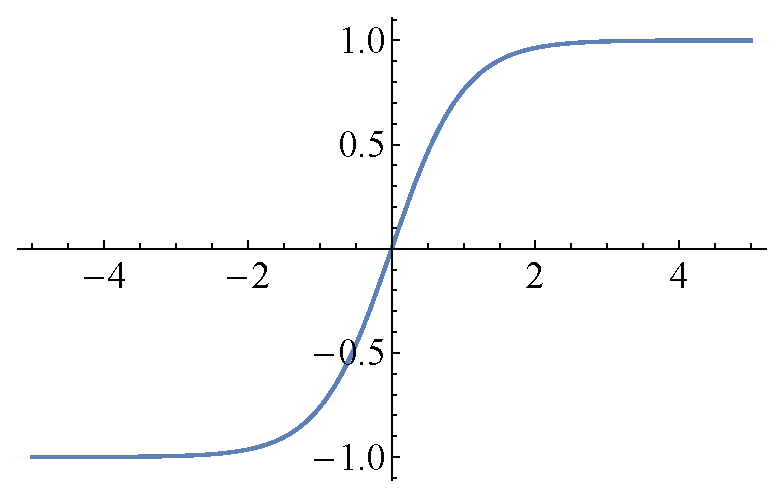
\includegraphics{Figure-5.eps}
		\caption{$f(x)$的一个图像}
	\end{marginfigure}
	令\green{\reff{tanh}}中$\varepsilon\rightarrow 0$,可知$f(x)$可导,且$f'(x)=[1-(f(x))^2]f'(0)$。求解该方程(称为微分方程)可得:$$f(x)=\dfrac{e^{f'(0)x}-e^{-f'(0)x}}{e^{f'(0)x}+e^{-f'(0)x}}=\tanh(f'(0)x)$$		
	至此我们可以发现,函数的基本形态已经大体由②确定了,①中我们只使用了$f(x)$有界这一条件,因此①完全可以放宽为有界性。So what if $f'(0)$ remains undefined?
\end{kaiti}\par\vspace{1em}

\begin{que}
	函数$f(x)$满足①$f(a+b)=f(a)\cdot f(b)$,②$f(4)=16$,$m,n$为互质整数,$n\neq 0$,求$f\left(\dfrac{m}{n}\right)$的值。
\end{que}
\sol 令$a=b=0$得$f(0)=[f(0)]^2\Rightarrow f(0)=0,1$。若$f(0)=0$,再令$b=0$,可得$f(a+0)=f(a)=f(a)f(0)=0\Rightarrow f(x)\equiv 0$,这与②矛盾。以下就$f(0)=1$时情况作讨论。令$b=-a$可得$f(-a)=\dfrac{1}{f(a)}$,再令$a=b=\dfrac{x}{2}$,可得$f(x)=\left[f\left(\dfrac{x}{2}\right)\right]^2\geqslant 0$,再根据条件②可知$f(1)=2$。\par
因此$f\left(\dfrac{m}{n}\right)=\left[f\left(\dfrac{1}{n}\right)\right]^m=\left[f\left(1\right)\right]^{\frac{m}{n}}=\res{2^\frac{m}{n}}$。\par\hfill\tg{抽象函数\ 分析}\easy\par
\begin{kaiti}
	本题中抛却条件②,我们可以知道一个更纯粹的事实:满足$f(a+b)=f(a)\cdot f(b)$的函数$f(x)$至少在有理数域上为指数函数。同\reff{tanh}一样地,我们添加$f(x)$在$x=0$处连续且可导以及全定义域上有界的条件,便可将这一事实拓展到整个实数域(忽略平凡解$f(x)\equiv 0$):注意到随着$\varepsilon\rightarrow 0$,$$|f(x+\varepsilon)-f(x)|=\underbrace{|f(x)|}_{<M}\underbrace{|[f(\varepsilon)-1]|}_{\rightarrow 0}\rightarrow 0$$因此$f(x)$在整个定义域内连续;注意到随着$\varepsilon\rightarrow 0$,
	$$\dfrac{f(x+\varepsilon)-f(x)}{\varepsilon}=f(x)\dfrac{f(\varepsilon)-f(0)}{\varepsilon}\rightarrow f(x)f'(0)<\infty$$因此$f(x)$在整个定义域内可导,且$f'(x)=f(x)f'(0)$,解这一方程可得,$f(x)=e^{f'(0)x}$,这是指数函数。
\end{kaiti}\par

\begin{que}
	已知函数$f(x)$满足:①对任意$x,y\in\mathbb{R}$,有$f(xy)=f(x)f(y)$;②$f(-1)=1$,$f(27)=9$;③$\forall x\in[0,1),f(x)\in[0,1)$。
	\begin{enumerate}
		\item 判断$f(x)$的奇偶性。
		\item 判断$f(x)$在$[0,+\infty)$的单调性。
		\item 若$a\geqslant 0$,且$f(a+1)\leqslant\sqrt[3]{9}$,求$a$的取值范围。
	\end{enumerate}
\end{que}
\sol \begin{enumerate}
	\item 令$y=-1$,得$f(-x)=f(x)f(-1)=f(x)$,$f(x)$为偶函数。
	\item 令$x=y=0$,得$f(0)=0$。$\forall x\in\mathbb{R}^+$,$f(x)=[f(\sqrt{x})]^2\geq 0$。若存在不为零的正实数$x_0$使得$f(x_0)=0$,那末\sidenote{应当注意到,根据题设,$f(x)<\infty$,即$f(x)$定义域为$\mathbb{R}$。}$9=f(27)=f(x_0)f\left(\dfrac{27}{x_0}=0\right)$,矛盾,因此$\forall x>0$,$f(x)>0$。\par
	令$x_1>x_2>0$,$x=x_1$,$y=\dfrac{x_2}{x_1}$,得
	$$f\left(x_1\cdot\dfrac{x_2}{x_1}\right)=\underbrace{f(x_2)}_{>0}=\underbrace{f(x_1)}_{>0}\underbrace{f\left(\dfrac{x_2}{x_1}\right)}_{\in[0,1)}<f(x_1)$$
	因此$f(x)$在$[0,+\infty)$上(严格)单调增,在$(-\infty,0]$上(严格)单调减。
	\item $f((a+1)^2)=[f(a+1)]^3\leqslant 9\ \Leftrightarrow\ (a+1)^3\in[0,27]\ \Leftrightarrow\ \res{a\in[1,2]}$
\end{enumerate}\par\hfill\tg{抽象函数\ 分析}\easy

\begin{que}
	设$A$是定义在$[2,4]$上且满足如下条件的函数$\varphi(x)$的集合:\\
	①\ $\forall x\in[1,2]$,有$\varphi(2x)\in(1,2)$。\\
	②\ 存在常数$L(0<L<1)$,使得对于任意$x_1,x_2\in[1,2]$,都有$|\varphi(2x_1)-\varphi(2x_2)|\leqslant L|x_1-x_2|$。
	\begin{enumerate}
		\item 设$\varphi(2x)=\sqrt[3]{1+x}$,$x\in[2,4]$,证明:$\varphi\in A$。
		\item 设$\varphi\in A$,如果存在$x_0\in(1,2)$,使得$x_0=\varphi(2x_0)$,那么这样的$x_0$是唯一的。
		\item 设$\varphi\in A$,任取$x_1\in(1,2)$,令$x_{n+1}=\varphi(2x_n),n\in\mathbb{N}^+$,证明:给定正整数$k$,那末对于任意的正整数$p$,不等式$$|x_{k+p}-x_{p}|\leqslant \dfrac{L^{k+1}}{1-L}|x_2-x_1|$$成立。
	\end{enumerate}
\end{que}
\sol \begin{enumerate}
	\item \sidenote{本题出题背景涉及到了柯西列、李普希兹条件和柯西中值定理,但最终成题却非常简单。有兴趣可对这些名词稍作了解。应当注意到$\dfrac{f(x_1)-f(x_2)}{x_1-x_2}$为割线斜率。若可导函数割线斜率有界,那末其导函数必有界。}显然$x\in[1,2]$时,$\varphi(2x)=\sqrt[3]{1+x}\in[\sqrt[3]{2},\sqrt[3]{3}]\subset(1,2)$;对于任意$x_1,x_2\in[1,2]$,有
	$$\begin{aligned}
		\left|\sqrt[3]{1+x_1}-\sqrt[3]{1+x_2}\right|&=\dfrac{|x_1-x_2|}{|(1+x_1)^{2/3}+(1+x_2)^{2/3}+(1+x_1)^{1/3}(1+x_2)^{1/3}|}\\
		&\leqslant\dfrac{|x_1-x_2|}{|3\times 2^{2/3}|}=L|x_1-x_2|
	\end{aligned}$$
	其中$L=\dfrac{1}{3\times 2^{2/3}}\in(0,1)$符合要求,因此$\varphi \in A$。
	\item 假设$\exists x_1,x_2\in(1,2)$,$x_1\neq x_2$,$x_1=\varphi(2x_1)$,$x_2=\varphi(2x_2)$,那末
	$|\varphi(2x_1)-\varphi(2x_2)|=|x_1-x_2|$,这与$\varphi(x)\in A$前提下应满足的②矛盾,因此唯一性得以说明。
	\item 注意到这样一个事实:$\forall m\in\mathbb{N}^+$,
	$$|x_{m+1}-x_m|=|\varphi(2x_{m})-\varphi(2x_{m-1})|\leqslant L|x_m-x_{m-1}|\leqslant\cdots\leqslant L^{m-1}|x_2-x_1|$$ 因此,
	$$\begin{aligned}
		|x_{k+p}-x_k|&=|(x_{k+p}-x_{k+p-1})+(x_{k+p-1}-x_{k+p-2})+\cdots+(x_{k+1}-x_k)|\\
		&\leqslant |x_{k+p}-x_{k+p-1}|+|x_{k+p-1}-x_{k+p-2}|+\cdots+|x_{k+1}-x_k|\\
		&\leqslant (L_{k+p-2}+L_{k+p-3}+\cdots+L_{k-1})|x_2-x_1|\\
		&=\dfrac{L_{k-1}(1-L^{p})}{1-L}|x_2-x_1|\\&\leqslant \dfrac{L_{k-1}}{1-L}|x_2-x_1|
	\end{aligned}$$
\end{enumerate}\par\hfill\tg{抽象函数\ 分析}\normal\par

%%%%%%%%%%%%%%%%%%%%%%%%%%%%%%%%%%%%%%%%%%%%%%%%
\section{求取参变量范围的综合题目}
\begin{que}
	已知函数$f(x)=\dfrac{a}{2}x^2+(a+1)x+2\ln(x-1)$,
	\begin{enumerate}
		\item 若曲线$y=f(x)$在点$(2,f(2))$处的切线与直线$2x-y+1=0$平行,求出这条切线的方程。
		\item 讨论函数$f(x)$的单调区间。
		\item 若对于任意$x\in(1,+\infty)$都有$f(x)<-2$,求实数$a$的取值范围。
	\end{enumerate}
\end{que}
\sol 易知$f(x)$定义域$x\in (1,+\infty)$,
	\begin{enumerate}
		\item $f'(x)=ax+a+1+\dfrac{2}{x-1}$$\ \Rightarrow\ $$f'(2)=3a+3=2$,故$a=-\dfrac{1}{3}$,$f(2)=\dfrac{2}{3}$,故切线方程为$$y-\dfrac{2}{3}=2(x-2)\quad\Leftrightarrow\quad \res{3y-6x+10=0}$$
		\item 由于$a=-\dfrac{1}{3}$,故$f(x)=-\dfrac{1}{6}x^2+\dfrac{2}{3}x+2\ln(x-1)$,$f'(x)=-\dfrac{1}{3}x+\dfrac{2}{3}+\dfrac{2}{x-1}$,$f''(x)=-\dfrac{1}{3}-\dfrac{2}{(x-1)^2}<0$,易知%
		$$f'(x)\leqslant 0\ \Leftrightarrow x \in [4,+\infty)\qquad f'(x)\geqslant 0\ \Leftrightarrow x \in (1,4]$$
		故$f(x)$在$(1,4]$上单调增,在$[4,+\infty)$上单调减。
		\item \blue{(方法一)}显然,$a<0$。分离变量得\sidenote{一般都是有两种方法求解此类题。一是将$f(x)$的最大值以$a$表达出来为$g(a)$,再解关于$a$的不等式方程;二是分离变量为$f_1(a) < f_2(x)$后解不等式$f_1(a) < \min f_2(x)$。}
		$$\begin{aligned}\text{原式}\ &\Leftrightarrow\ a(x^2+2x)<-4-2x-4\ln(x-1)\\
			&\Leftrightarrow\ a<-\dfrac{4+2x+4\ln(x-1)}{x^2+2x}=-g(x)\qquad{\purple{\footnotesize{x^2+2x=(x+1)^2-1>3>0}}}\end{aligned}
			$$
		\begin{marginfigure}
			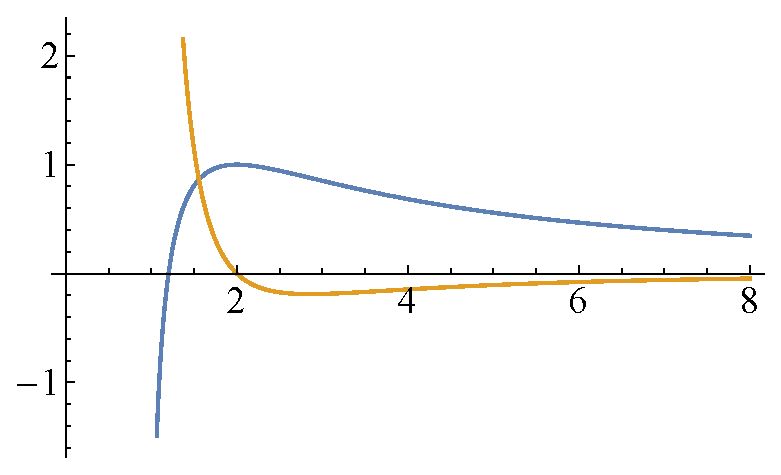
\includegraphics{Figure-1.eps}
			\caption{$g'(x)$的图像}
		\end{marginfigure}
		若我们能够求得$\max g(x)$,则解即为$a < -\max g(x)$。为方便书写,记$\ln0=-\infty$,
		$$g'(x)=-\dfrac{\overbrace{2(x+1)}^{>0}(x^2-4+4(x-1)\ln(x-1))}{\underbrace{x^2(x+2)^2(x-1)}_{>0}}=-\dfrac{2(x+1)(x^2-4+4h(x))}{x^2(x+2)^2(x-1)}$$
		注意到$g'(2)=h(2)=h(1)=0$\ \sidenote{当$x$接近$0$时,$x\ln x$接近$0$。这一点可用不等式$$x-1\geqslant\ln x\geqslant-\dfrac{2}{\sqrt{x}}$$证明。因此我们始终「不妨可设」$0\ln0=0$进行补充定义。为使叙述简便和理解方便,方法一过程中补充定义了边界值,实际考试中应当小心仔细说明。}$g'(2)=h(2)=h(1)=0$。而$h'(x)=\ln(x-1)+1$,故$h(x)$在$\left(1,1+\dfrac{1}{e}\right)$上单调减,在$\left(1+\dfrac{1}{e},+\infty\right)$上单调增,进而$$h(x)<0,x^2-4<0\ \Leftrightarrow\ x\in(1,2)\quad h(x)>0,x^2-4>0\ \Leftrightarrow\ x\in(2,+\infty)$$
		可推知$g(x)$在$(1,2)$上单调增,在$(2,+\infty)$上单调减,$a<-\max g(x)=-g(2)=\res{-1}$。\par\vspace{0.5em}
		\blue{(方法二)}显然,$a<0$。$f'(x)=0\ \Leftrightarrow\ x_1=-1\text{(舍)}\ \ x_2=\dfrac{a-1}{a}>1$,故$f(x)$在$(1,+\infty)$上必然先增后减,
			$$\max f(x)=f\left(\dfrac{a-1}{a}\right)=-1-\dfrac{1}{2a}+\dfrac{3a}{2}+2\ln\left(-\dfrac{1}{a}\right)=g(a)<-2\ \Rightarrow\ a<0$$
			$$g'(a)=\dfrac{3}{2}+\dfrac{1}{2a^2}-\dfrac{2}{a}>0\ \Rightarrow\ g(a)\text{单调增}$$
		注意到$g(-1)=-2$,故所求$a$的取值范围为$\res{a<-1}$。\hfill\tg{参数范围}\easy
	\end{enumerate}

\begin{que}
	设函数$f(x)=2\ln(x-1)-(x-1)^2$,
	\begin{enumerate}
		\item 求函数的单调递增区间。
		\item 若关于函数$x$的方程$f(x)+x^2-3x-a=0$在区间$[2,4]$上有两个相异的实根,求实数$a$的取值范围。
	\end{enumerate}
\end{que}
\sol \begin{enumerate}
	\item $f'(x)=\dfrac{2}{x-1}-2(x-1)$,故结合定义域$x>1$知$f'(x)\geqslant 0\Rightarrow x\in (1,2]$,$f'(x)\leqslant 0\Rightarrow x\in[2,+\infty)$,$f(x)$在$(1,2]$上单调增,在$[2,\infty)$上单调减。
	\item 	
	\begin{marginfigure}
		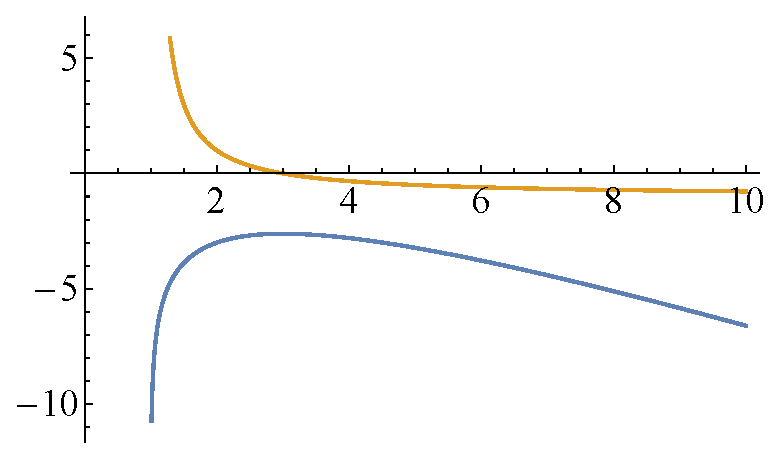
\includegraphics{Figure-2.eps}
		\caption{$g(x)=2\ln(x-1)-x-1$(蓝)及其导函数(橙)的图像}
	\end{marginfigure} 改写原式为$a=f(x)+x^2-3x=2\ln(x-1)-x-1=g(x)$,由$g'(x)=\dfrac{2}{x-1}-1$知
	$$g(x)\text{单调增}\ \Leftrightarrow\ g'(x)\geqslant 0\ \Leftrightarrow x\in(1,3]\quad g(x)\text{单调减}\ \Leftrightarrow\ g'(x)\leqslant 0\ \Leftrightarrow x\in[3,+\infty)$$
	因此$\max g(x)=g(3)=2\ln2-4$。注意到当$x$趋近于$1$或$-\infty$时,$g(x)$均趋近于$-\infty$,我们可大致知道$g(x)$的图像形状,因此易知$a$的取值范围为$\res{a<2\ln2-4}$。\par\vspace{0.5em}\hfill\tg{参数范围\ 最值}\easy
\end{enumerate}
\begin{que}
	已知函数$f(x)=x^3-ax^2-a^2x+1$,$g(x)=1-4x-ax^2$,其中实数$a\neq 0$,
	\begin{enumerate}
		\item 求函数$f(x)$的单调区间。
		\item 当函数$y=f(x)$与$y=g(x)$的图像只有一个公共点且$g(x)$存在最小值时,记$g(x)$的最小值为$h(a)$,求$f(a)$的值域。
		\item 若$f(x)$与$g(x)$在区间$(-a,-a+2)$内均为增函数,求$a$的取值范围。
	\end{enumerate}
\end{que}
\sol \begin{enumerate}
	\item $f'(x)=3x^2-2ax-a^2=(3x+a)(x-a)=0$$\ \Rightarrow\ x_1=-\dfrac{a}{3}$,$x_2=a$,显然$a\neq0$时$x_1\neq x_2$。
	\begin{enumerate}
		\item 当$a>0$时,$x_2>x_1$,$f(x)$在$\left(-\infty,-\dfrac{a}{3}\right]$\textbf{和}$[a,+\infty)$上单调增,在$\left[-\dfrac{a}{3},a\right]$上单调减。
		\item 当$a<0$时,$x_2<x_1$,$f(x)$在$(-\infty,a]$\textbf{和}$\left[-\dfrac{a}{3},+\infty\right)$上单调增,在$\left[a,-\dfrac{a}{3}\right]$上单调减。
	\end{enumerate}
	\item $g(x)$存在最小值意味着$a>0$,由于$f(x)$与$g(x)$的次数不一,因此从两者图像上寻找「只有一个公共点」的情形是困难的,我们须得设差值函数$m(x)=f(x)-g(x)=x^3+(4-a^2)x$,公共点条件即转化为$m(x)$有且仅有一个零点\sidenote{涉及到函数图像相交的问题,均可转化为「交点处为差值函数零点$\Leftrightarrow$交点处函数值相同」的问题,这一过程将减少函数个数,从而简化问题。对于特殊图像,也可从图像特征入手。}。由于$0$为$m(x)$的一个零点,$m(x)$为中心对称的奇函数,故若使$m(x)$零点唯一,$m(x)$必然单调增,即$$m'(0)=[3x^2+(4-a^2)]_{x=0}=4-a^2\geqslant 0\ \Rightarrow\ \res{a\in(0,2]}$$
	\item 记$I=(-a,-a+2)$。$g'(x)=-4-2ax$,使$g(x)$在$I$上单调增有
	$$\left\{\begin{aligned}&g'(-a)=-4+2a^2\geqslant 0\\ &g'(-a+2)=2a^2-4a-4\geqslant 0\end{aligned}\right.\quad\Leftrightarrow\quad a\in(-\infty,-\sqrt{2}]\cup[1+\sqrt{3},+\infty)$$
	在这一范围基础上,注意到$I$的长度为$|I|=2$,而$f'(x)$两根$x_1,x_2$满足$x_1+x_2=\dfrac{2a}{3}$,$x_1x_2=-\dfrac{a^2}{3}$,故$$|x_1-x_2|=\sqrt{(x_1+x_2)^2-4x_1x_2}=\dfrac{4a^2}{3}\geqslant\dfrac{4\times(\sqrt{2})^2}{3}=\dfrac{16}{3}>2=|I|$$
	因此$f(x)$在$I$上不可能有三段增减区间,故只需使
	$$\left\{\begin{aligned}&f'(-a)=4a^2 \geqslant 0\\ &f'(-a+2)=4(a-3)(a-1)\geqslant 0\end{aligned}\right.\quad\Leftrightarrow\quad a\in(-\infty,1]\cup[3,+\infty)$$
	综上,可知$a$的取值范围为$\res{a\in(-\infty,-\sqrt{2}]\cup[3,+\infty)}$。\par\vspace{0.5em}\hfill\tg{取值范围\ 交点}\normal
\end{enumerate}

\begin{que}
	设$a$为实数,记函数$f(x)=a\sqrt{1-x^2}+\sqrt{1+x}+\sqrt{1-x}$的最大值为$g(a)$。
	\begin{enumerate}
		\item 设$t=\sqrt{1+x}+\sqrt{1-x}$,求$t$的取值范围,并把$f(x)$改写为$t$的函数$m(t)$。
		\item 求出$g(a)$。
		\item 求出满足$g(a)=g\left(\dfrac{1}{a}\right)$的所有实数$a$。
	\end{enumerate}
\end{que}
\sol \begin{enumerate}
	\item 显然$x\in [-1,1]$,$t\geqslant 0$,$t^2=2+2\sqrt{1-x^2}\in[2,4]\Rightarrow t\in[\sqrt{2},2]$。同时我们得到$\sqrt{1-x^2}=\dfrac{1}{2}t^2-1$,进而$$f(x)=a\left(\dfrac{1}{2}t^2-1\right)+t=\res{\dfrac{a}{2}t^2+t-a=m(t)}$$
	\item $m(t)$对称轴$t_0=-\dfrac{1}{a}(a\neq 0)$,$t\in[\sqrt{2},2]$。
	\begin{enumerate}
		\item 若$a=0$,则$m(t)$退化为单调增的一次函数\sidenote{一次函数可以视为退化的二次函数,直线和双直线可以视为退化的二次曲线。基于这一点我们应当有这样的先验直觉:$g(a)$必然连续。事实上也的确连续。},最大值$g(0)=m(2)=2$。
		\item 若$a>0$,则$m(t)$为开口向上,对称轴在$y$轴左侧的二次函数,最大值$g(a)=m(2)=a+2$。
		\item 若$a\in\left[-\dfrac{\sqrt{2}}{2},-\dfrac{1}{2}\right]$,则$m(t)$为开口向下,对称轴$t_0\in[\sqrt{2},2]$的二次函数,最大值$g(a)=m(t_0)=-a-\dfrac{1}{2a}$。
		\item 若$a\in\left(-\dfrac{\sqrt{2}}{2},0\right)$,则$m(t)$为开口向下,对称轴$t_0<\sqrt{2}$的二次函数,最大值$g(a)=m(\sqrt{2})=\sqrt{2}$。
		\item 若$a\in\left(-\infty,-\dfrac{1}{2}\right)$,则$m(t)$为开口向下,对称轴$t_0>2$的二次函数,最大值$g(a)=m(2)=2+a$。
	\end{enumerate}
	因此:$g(a)=\left\{\begin{aligned}
		&a+2&a\in\left(-\dfrac{1}{2},+\infty\right)\\
		&-a-\dfrac{1}{2a}&a\in\left[-\dfrac{\sqrt{2}}{2},-\dfrac{1}{2}\right]\\
		&\sqrt{2}&a\in\left(-\infty,-\dfrac{\sqrt{2}}{2}\right)
	\end{aligned}\right.$。\begin{marginfigure}
		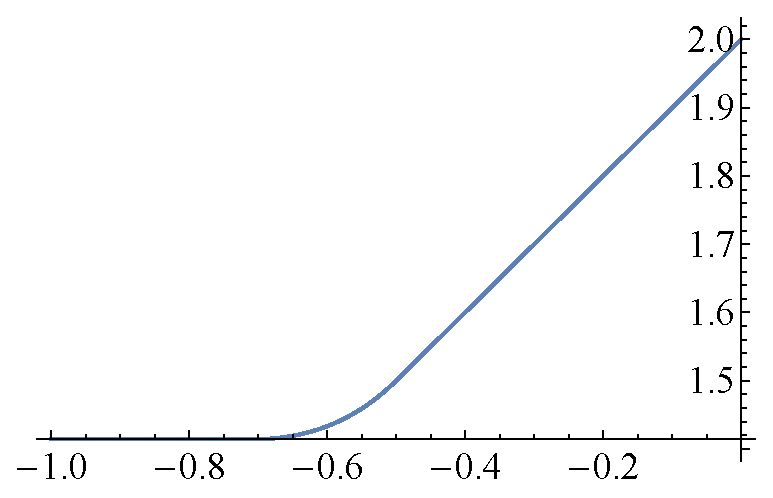
\includegraphics{Figure-4.eps}
		\caption{$g(x)$在$[-1,0]$上的图像。可以看到是连续的。}
	\end{marginfigure}
	\item 由$(a+2)|_{a=-1/2}=\left(-a-\dfrac{1}{2a}\right)|_{a=-1/2}=\dfrac{3}{2}$,$\sqrt{2}=\left(-a-\dfrac{1}{2a}\right)|_{a=-1/\sqrt{2}}=\sqrt{2}$知$g(a)$是连续的。分段求导可知,$g(a)$当$a\geqslant-\dfrac{\sqrt{2}}{2}$时严格单调增,那末
	$$g(a)=g\left(\dfrac{1}{a}\right)\ \Leftrightarrow\ a=\dfrac{1}{a}\text{\ 或\ }a,\dfrac{1}{a}\leqslant-\dfrac{\sqrt{2}}{2}\ \Leftrightarrow\ \res{a\in\left[-\sqrt{2},-\dfrac{\sqrt{2}}{2}\right]\cup\{1\}}$$
\end{enumerate}\par\hfill\tg{取值范围}\easy

\begin{que}
	已知函数$f(x)=\dfrac{1+x}{1-x}e^{-ax}$,
	\begin{enumerate}
		\item 设$a>0$,讨论$y=f(x)$的单调性。
		\item 若对任意$x\in(0,1)$恒有$f(x)>1$,求$a$的取值范围。
	\end{enumerate}
\end{que}
\sol $f'(x)=\dfrac{a\left(x^2+\dfrac{2-a}{a}\right)}{(x-1)^2}e^{-ax}$
\begin{enumerate}
	\item 
	\begin{enumerate}
		\item 若$a\in(0,2]$,则$\dfrac{2-a}{a}\geqslant 0$,$f'(x)\geqslant 0$恒成立,$f(x)$在$(-\infty,1)$\textbf{和}$(1,+\infty)$上单调增。
		\item 若$a>2$,则$f'(x)=0\ \Leftrightarrow\ x_1=-\sqrt{\dfrac{a-2}{a}},\ x_2=\sqrt{\dfrac{a-2}{a}}<1$,因此$f(x)$在$\left(-\infty,-\sqrt{\dfrac{a-2}{a}}\right]$、$\left[\sqrt{\dfrac{a-2}{a}},1\right)$\textbf{和}$(1,+\infty)$上单调增,在$\left[-\sqrt{\dfrac{a-2}{a}},\sqrt{\dfrac{a-2}{a}}\right]$单调减。
	\end{enumerate}
	\item \blue{(方法一)}$(0,1)$上,$f'(x)=\dfrac{2+a\overbrace{(x^2-1)}^{\in(-1,0)}}{(x-1)^2}e^{-ax}$
	\begin{enumerate}
		\item 若$a\leqslant 2$,则$2+a(x^2-1)\geqslant 0\Rightarrow f'(x)$单调增$\Rightarrow f(x)>f(0)=1$,$x\in(0,1)$,这是符合题意的。
		\item 若$a>2$,则$f'(0)<0$,$f(x)$先严格单调减后单调增,而$f(0)=1$,因此必存在$1>x_0>0$\ s.t.\ $f(x_0)<1$,这是不符合题意的,因此$\res{a\leqslant 2}$。
	\end{enumerate}
	\blue{(方法二\ 分离变量法)}易知$x\in(0,1)$则$\dfrac{1+x}{1-x}>0$。$f(x)$取对数知$\forall x\in(0,1)$,$\ln f(x)=\ln(1+x)-\ln(1-x)-ax>\ln 1=0$,
	$$a<\min_{x\in(0,1)}\dfrac{\ln(1+x)}{x}-\dfrac{\ln(1-x)}{x}=\min_{x\in(0,1)} g(x)$$
	$g'(x)=\dfrac{1}{x^2}\left[\dfrac{2x}{1-x^2}+\ln\left(\dfrac{1-x}{1+x}\right)\right]=\dfrac{1}{x^2}h(x)$,注意到$h'(x)=\dfrac{4x^2}{(x^2-1)^2}>0$,$h(0)=0$,故在$(0,1)$上$g'(x)>0$,$g(x)$单调增。现在我们须找出$x$趋近于$0$时,$g(x)$趋近的值。事实上,可利用以下不等式\sidenote{这里的不等式均源于多项式级数展开的截取,证明大同小异,非常简单,故不再证明。下诸题同。}:
	$$\begin{aligned}&\quad x-\dfrac{x^2}{2}\leqslant\ln(1+x)\leqslant x\\
		&\Rightarrow\ \left(x-\dfrac{x^2}{2}\right)-(-x)\leqslant\ln(1+x)-\ln(1-x)\leqslant x-\left(-x-\dfrac{x^2}{2}\right)\\
		&\Leftrightarrow 2x-\dfrac{x^2}{2}\leqslant\ln\left(\dfrac{1+x}{1-x}\right)\leqslant 2x+\dfrac{x^2}{2}\qquad\purple{\text{\footnotesize 这是一个非常常用的不等式}}\\
		&\Leftrightarrow 2-\dfrac{x}{2}\leqslant g(x)\leqslant 2+\dfrac{x}{2}\end{aligned}$$
	因此\sidenote{「趋于」这一词引入于数学教材定积分一章,是否在考试中可以使用视要求而定。不能使用的情况下可以如下叙述:\begin{enumerate}
		\item $g(x)$是连续的,且单调增至无穷。对于任意大于$2$的值,譬如$2+\epsilon$,$\epsilon>0$,均可取适当的$x>0$,使得$g(x)\leqslant 2+\dfrac{x^2}{2} < 2+\epsilon$,这样由$g(x)$单调增知$g(x)$必可取到$2+\epsilon$。
		\item 假设$g(x)$可取到任意小于$2$的值,譬如$g(x_0)=2-\epsilon$,$\epsilon>0$,均可取适当的$x_0>x_1>0$,使得$g(x_1)\geqslant 2-\dfrac{x^2}{2} > 2-\epsilon$,这与$g(x)$单调增矛盾。
		\item 因此$g(x)$必然严格大于$2$。
	\end{enumerate}}当$x$趋于$0$时,$g(x)$趋于$2$,而这一最小值是取不到的。因此$\res{a\leqslant 2}$。
\end{enumerate}\par\hfill\gk\tg{取值范围\ 极限}\easy

%%%%%%%%%%%%%%%%%%%%%%%%%%%%%%%%%%%%%%%%%%%%%%%%
\section{引出不等式证明的综合题目}
关于此类题目一些常用不等式的统一证明:
\begin{enumerate}
	\item \labeltext[\green{[IEQ\ 1]}]{[IEQ\ 1]$\mathbf{e^x\geqslant 1+x}$}{ieq1} \par
	该式截取自$e^x$的麦克劳林展开式$$e^x=1+x+\dfrac{x^2}{2!}+\dfrac{x^3}{3!}+\cdots+\dfrac{x^n}{n!}+\cdots$$前两项,截取更多项时证明相仿,只需多求几次导数,不赘述。\par
	令$g(x)=e^x-(1+x)$,则$g'(x)=e^x-1$,$g''(x)=e^x>0$,因此$g'(x)$单调增,又$g'(0)=0$,因此$g(x)$在$(-\infty,0)$上单调递减,在$(0,+\infty)$上单调递增,$\forall x\in\mathbb{R}$,$$g(x)\geqslant g(0)=0\ \Leftrightarrow\ e^x\geqslant 1+x$$
	当仅当$x=0$时取等。
	 \item \labeltext[\green{[IEQ\ 2]}]{[IEQ\ 2]$\mathbf{\ln(1+x)\leqslant x}\ (x>-1),\mathbf{\ln(1+x)\geqslant x-\dfrac{x^2}{2}}\ (x\geqslant 0)$}{ieq2} \par
	该式截取自$\ln(1+x)$的麦克劳林展开式$$\ln(1+x)=x-\dfrac{x^2}{2}+\dfrac{x^3}{3}-\cdots+(-1)^{n+1}\dfrac{x^n}{n}+\cdots$$前两项,截取更多项时证明相仿,只需多求几次导数,不赘述,这里我们证第二式。\par
	令$g(x)=\ln(1+x)-x+\dfrac{x^2}{2!}$,则$g'(x)=\dfrac{1}{1+x}-1+x$,$g''(x)=-\dfrac{1}{(1+x)^2}+1\geqslant 0$,$g'(0)=0$,因此$g(x)$在$[0,+\infty)$上单调增,$\forall x\geqslant 0$,$$g(x)\geqslant 0 \ \Rightarrow\ \ln(1+x)\geqslant x-\dfrac{x^2}{2}$$
	当仅当$x=0$时取等。
	\item \labeltext[\green{[IEQ\ 3]}]{[IEQ\ 3]$\mathbf{\ln x \leqslant 1-\dfrac{1}{x}}$}{ieq3} \par
	令$g(x)=\ln x-1+\dfrac{1}{x}$,可证$g(x)\geqslant g(1)=0$,因此$\forall x\in \mathbb{R}^+,\ \ln x\geqslant 1-\dfrac{1}{x}$。
	%\item \labeltext[[IEQ\ 3]]{$\mathbf{\ }$}{ieq2} \par
\end{enumerate}
\begin{que}
	已知函数$f(x)=\dfrac{a(1-x)}{x}\ln(1-x),a\in\mathbb{R}$,$e$为自然常数。
	\begin{enumerate}
		\item 求$f(x)$在区间$\left[1-e^2,1-e\right]$上的最值。
		\item 比较$\left(1+\dfrac{1}{2!}\right)\left(1+\dfrac{1}{3!}\right)\cdots\left(1+\dfrac{1}{n!}\right)$与$e$的大小。
	\end{enumerate}
\end{que}
\sol \begin{enumerate}
	\item 导数$f'(x)=-\dfrac{a(x+\ln(1-x))}{x^2}$。由\ref{ieq2},$\ln(1-x)\leqslant -x$,因此
	\begin{enumerate}
		\item 若$a=0$,则$f(x)\equiv 0$,所求最值$\res{\max f(x)=0}$。
		\item 若$a>0$,则$x+\ln(1-x)\leqslant 0$,$f'(x)\geqslant 0$,$f(x)$单调增,所求最值
		$$\max_{[1-e^2,1-e]} f(x)=f(1-e)=\res{\dfrac{ae}{1-e}}\quad \min_{[1-e^2,1-e]}f(x)=f(1-e^2)=\res{\dfrac{2ae^2}{1-e^2}}$$
		 \item 若$a<0$,则$f'(x)\leqslant 0$,$f(x)$单调减,所求最值
		$$\min_{[1-e^2,1-e]} f(x)=f(1-e)=\res{\dfrac{ae}{1-e}}\quad \max_{[1-e^2,1-e]}f(x)=f(1-e^2)=\res{\dfrac{2ae^2}{1-e^2}}$$
	\end{enumerate}
	\item 由\ref{ieq2},$\ln(1+x)\leqslant x$,因此$$
		\begin{aligned}&\ln\left[\left(1+\dfrac{1}{2!}\right)\left(1+\dfrac{1}{3!}\right)\cdots\left(1+\dfrac{1}{n!}\right)\right]\\=\ &\ln\left(1+\dfrac{1}{2!}\right)+\ln\left(1+\dfrac{1}{3}\right)+\cdots+\ln\left(1+\dfrac{1}{n!}\right)\\\leqslant\ &\dfrac{1}{2!}+\dfrac{1}{3!}+\cdots+\dfrac{1}{n!}\\\leqslant\ &\dfrac{1}{1\times 2}+\dfrac{1}{2\times 3}+\cdots +\dfrac{1}{(n-1)n}\\=\ &1-\dfrac{1}{n}<1=\ln e \\
		\Rightarrow\ &\res{\left(1+\dfrac{1}{2!}\right)\left(1+\dfrac{1}{3!}\right)\cdots\left(1+\dfrac{1}{n!}\right)<e}\end{aligned}$$
\end{enumerate}\par\hfill\tg{不等式}\easy

\begin{que}
	已知函数$f(x)=\ln ax-\dfrac{x-1}{x}$。
	\begin{enumerate}
		\item 求此函数的单调区间与最值。
		\item 求证:对于任意正整数$n$,均有:$$1+\dfrac{1}{2}+\dfrac{1}{3}+\cdots+\dfrac{1}{n}> \ln\dfrac{e^n}{n!}$$
		\item 当$a=1$时,过点$(1,-1)$是否存在$y=f(x)$图像的切线?若存在,有多少条?若不存在,阐明理由。
	\end{enumerate}
\end{que}
\sol 	\begin{enumerate}
	\item $f'(x)=\dfrac{1}{x}\left(1-\dfrac{1}{x}\right)=0 \Rightarrow x=1$。若$a>0$,则$x>0$,$f(x)$在$(0,1)$上单调递减,在$[1,+\infty)$上单调递增。最小值$\min f(x)=f(1)=\ln a$,无最大值;若$a<0$,则$x<0$,$f(x)$在$\mathbb{R}^-$上单调递减,无最值。
	\item 由上小题结论(也即\ref{ieq3}),若取$a>0$,则$\ln ax-1+\dfrac{1}{x}\geqslant\ln a\Rightarrow \dfrac{1}{x}\geqslant 1-\ln x$,当仅当$x=1$时取等,因此$$1+\dfrac{1}{2}+\cdots+\dfrac{1}{n}> n-\ln\dfrac{1}{n!}=\ln\dfrac{e^n}{n!}$$
	\item $a=1$条件下,$x>0$,$f(x)$在$(x_0,f(x_0))$处切线方程可写为:$y-f(x_0)=\dfrac{x_0-1}{x_0^2}(x-x_0)$。假使该切线过点$(1,-1)$,则	
	\begin{marginfigure}
		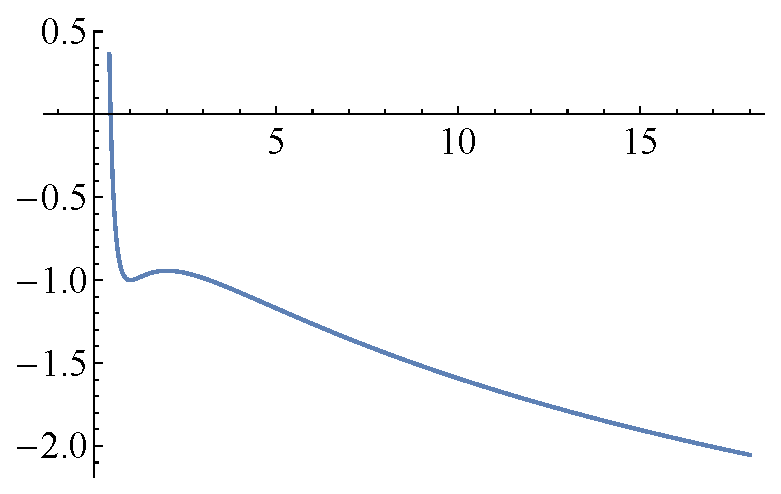
\includegraphics{Figure-6.eps}
		\caption{$g(x)$的图像}
	\end{marginfigure}$$-1-f(x_0)=\dfrac{x_0-1}{x_0^2}(1-x_0)\quad\Rightarrow\quad1-\dfrac{3}{x_0}+\dfrac{1}{x_0^2}-\ln x_0=g(x_0)=0$$
	由于$g'(x)=-\dfrac{2}{x}\left(\dfrac{1}{x}-1\right)\left(\dfrac{1}{x}-\dfrac{1}{2}\right)=0\Rightarrow x_1=1,x_2=2$,故$g(x)$在$(0,1)$上单调减,在$(1,2)$上单调增,在$(2,+\infty)$上单调减,$g(1)=-1<0$,$g(0)=+\infty$,$g(2)=-\ln 2-\dfrac{1}{4}<0$,$g(+\infty)=-\infty$,因此$g(x)$有且仅有一个零点,这意味着所求切线存在且仅存在$\res{1}$条。
\end{enumerate}\par\hfill\tg{不等式\ 切线方程}\easy

\begin{que}
	设函数$f(x)=1-e^{-x}$,函数$g(x)=\dfrac{x}{ax+1}$,其中$a\in\mathbb{R}$,$e$为自然常数。
	\begin{enumerate}
		\item 当$a=0$时,求函数$h(x)=f'(x)g(x)$的极值。
		\item 若$f(x)\leqslant g(x)$在$[0,+\infty)$上恒成立,求实数$a$的取值范围。
		\item 设$n\in\mathbb{N}^+$,求证:($\exp x=e^x$)$$\exp\left(2n-\sum_{k=1}^n\dfrac{4}{k+1}\right)\leqslant n!\leqslant\exp\left(\dfrac{n(n-1)}{2}\right)$$
	\end{enumerate}
\end{que}
\sol \begin{enumerate}
	\item $f'(x)=e^{-x}$。$a=0$时,$h(x)=\dfrac{x}{x+1}e^{-x}$,$$h'(x)=\dfrac{1-x-x^2}{(1+x)^2}e^{-x}=0\ \Rightarrow\ x_1=\dfrac{-1-\sqrt{5}}{2},\ x_2=\dfrac{-1+\sqrt{5}}{2}$$
	$f''(x_1)>0$,$f''(x_2)<0$,因此极小值$f(x_1)=\res{\dfrac{3+\sqrt{5}}{2}e^{\frac{1+\sqrt{5}}{2}}}$,极大值$f(x_2)=\dfrac{3-\sqrt{5}}{2}e^{\frac{1-\sqrt{5}}{2}}$
	\item 显然首先$a\geqslant 0$。我们来说明$f(x)\leqslant g(x)$的必要条件为$a\leqslant \dfrac{1}{2}$。记$h_a(x)=g(x)-f(x)=\dfrac{x}{ax+1}+e^{-x}-1$,那末$$h_a^\prime(x)=\dfrac{1}{(1+ax)^2}-e^{-x}\quad h_a^{\prime\prime}(x)=e^{-x}-\dfrac{2a}{(1+ax)^3}$$若$a>\dfrac{1}{2}$,则$h_a^{\prime\prime}(0)=1-2a<0$,因此$h_a^\prime(x)$在$x=0$处单调减\sidenote{「在某点处单调减」似乎听起来很奇怪,其实并不然,这是一种「微观」的分析方法,也是数学分析中非常初等和常用的分析方法,常被放到高中题目中,但不要求滴水不漏的叙述。对于性质良好的函数$f$(至少连续),在某点,譬如$x_0$,周围的一个小邻域内是有保号性的,若$f(x_0)>0$,那末$\exists \delta>0$\ s.t.\ $\forall |\varepsilon|<\delta$,$f(x_0+\varepsilon)>0$。在本题中$h_a(x)$无穷连续可导,$h_a^{\prime\prime}(0)<0$意味着$\exists\delta>0$,$h_a^\prime(x)$至少在$[0,\delta]$上单调减。这就是(连续)函数在某点处单调性的意义。解答中这一手法非常常用。},$\exists \varepsilon>0$使得$h_a^\prime(\epsilon)<0\Rightarrow f(\varepsilon)>g(\varepsilon)$,这与题设矛盾,因此$a\leqslant \dfrac{1}{2}$。\par
	我们再来说明$0\leqslant a\leqslant\dfrac{1}{2}$的充分性。设$a\leqslant \dfrac{1}{2}$,注意到$$h_a(x)\geqslant\dfrac{2}{x+2}+e^{-x}-1=m(x)\quad m'(x)=\dfrac{4e^{-x}\left[\left(e^{\frac{x}{2}}\right)^2-\left(1+\dfrac{x}{2}\right)^2\right]}{(2+x)^2}$$
	由\ref{ieq1}知$\forall x\geqslant 0$,$e^\frac{x}{2}\geqslant 1+\dfrac{x}{2}$,故$$m'(x)\geqslant 0\ \Rightarrow\ m(x)\geqslant m(0)=0\ \Rightarrow\ h_a(x)\geqslant m(x)\geqslant0$$
	因此$\forall\ 0\leqslant a\leqslant \dfrac{1}{2}$,$g(x)\geqslant f(x)$,充分性得证。综上,$\res{a\in\left[0,\dfrac{1}{2}\right]}$。
	\item \blue{(方法一)}定义$h(x)=\ln x+\dfrac{4}{k+1}-2$,则$\forall x>0,\ h'(x)=\dfrac{(x-1)^2}{x(x+1)^2}\geqslant 0 $,$\forall x\geqslant 1,\ h(x)\geqslant h(1)=0$再结合\ref{ieq2}有$$\begin{aligned}&2-\dfrac{4}{x+1}\leqslant \ln n\leqslant \ln (x-1)\\\Leftrightarrow\ &2n-\sum_{k=1}^n\dfrac{4}{k+1}=\sum_{k=1}^n\leqslant \ln (n!)\leqslant\sum_{k=1}^n(k-1)=\dfrac{n(n-1)}{2}\\\Leftrightarrow\ &\exp\left(2n-\sum_{k=1}^n\dfrac{4}{k+1}\right)\leqslant n!\leqslant\exp\left(\dfrac{n(n-1)}{2}\right)\end{aligned}$$\par
	\blue{(方法二)}由上一小题知,$a=\dfrac{1}{2}$,$x\in[0,2)$时时,$$1-e^{-x}\leqslant \dfrac{x}{\dfrac{1}{2}x+a}\ \Leftrightarrow\ x\leqslant\ln\dfrac{2+x}{2-x}\in\mathbb{R}^+$$故可令$$n=\dfrac{2+x}{2-x}\ \Leftrightarrow\ x=2-\dfrac{4}{n+1}\ \Rightarrow\ \ln n\geqslant 2-\dfrac{4}{n+1}$$由第一小题知$$h(x)\leqslant h(1)\Rightarrow xe^{-x}\leqslant\dfrac{1}{e}\Rightarrow \ln x\leqslant x-1,\ \forall\ x\geqslant1$$,因此$2-\dfrac{4}{k+1}\leqslant \ln k\leqslant k-1$以下同方法一\sidenote{对于以证明不等式为目的的题目来说,虽然不等式的证明依赖于前行的小题,但对于简单的题目来说,可以不必拘泥于题目内容,独立证明也常常可以证出。}。
\end{enumerate}\par\hfill\tg{取值范围\ 不等式\ 分析}\normal

\begin{que}
	对于函数$f(x),x\in D$,若定义域上恒有$f'(x)>f(x)$成立,则称函数$f(x)$是$D$上的J函数。
	\begin{enumerate}
		\item 当$f(x)=me^x\ln x$是定义域上的J函数时,求$m$的取值范围。
		\item 若函数$g(x)$为$(0,+\infty)$上的J函数,
		\begin{enumerate}
			\item 试比较$g(a)$与$e^{a-1}g(1)$的大小。
			\item 求证:$\forall\ x_1,x_2,\cdots,x_n>1$,$$g(\ln(x_1+x_2+\cdots+x_n))>g(\ln x_1)+g(\ln x_1)+\cdots+g(\ln x_n)$$
		\end{enumerate}
	\end{enumerate}
\end{que}
\sol\sidenote{本题中万不可以出现$f''(x)$,这是由于题干中未给出$f(x)$存在二阶导数的条件。} \begin{enumerate}
	\item $f(x)=me^x\ln x$定义域为$\mathbb{R}+$,$$f'(x)=me^x\left(\ln x+\dfrac{1}{x}\right)>f(x)=me^x\ln x\ \Rightarrow\ \dfrac{me^x}{x}>0\ \Rightarrow\ \res{m>0}$$
	\item 设\sidenote{$f'(x)=f(x)$描述的函数为$f(x)=e^x$。直觉上,$f'(x)>f(x)$描述了比$e^x$增长快的函数,故设$h(x)=e^{-x}g(x)$。这一手法十分常用。}$h(x)=e^{-x}g(x)$,那末$h'(x)=e^{-x}\left[g'(x)-g(x)\right]>0$,故$h(x)$单调增。$a=1$时,$g(a)=e^{a-1}g(1)$;$a>1$时,$g(a)=e^ah(a)>e^ah(1)=e^{a-1}g(1)$;当$a<1$时,$g(a)=e^ah(a)<e^ah(1)=e^{a-1}g(1)$。\par
	不妨设$1<x_1\leqslant x_2\leqslant\cdots \leqslant x_n$,则由$h(x)$在$\mathbb{R}^+$上单调增知$$\begin{aligned}
		&\quad\  \forall 1\leqslant k\leqslant n,\ h(x_k)\leqslant h(x_n)\Rightarrow g(\ln x_k)\leqslant \dfrac{x_k}{x_n}g(\ln x_n)\\
		\Rightarrow\ &\quad\ g(\ln x_1)+g(ln x_2)+\cdots+g(\ln x_n)\leqslant \dfrac{x_1+x_2+\cdots+x_n}{x_n}g(\ln x_n)\\
		&=e^{\ln(x_1+x_2+\cdots+x_n)}h(\ln x_n)<e^{\ln(x_1+x_2+\cdots+x_n)}h(\ln(x_1+x_2+\cdots+x_n))\\
		&=g(ln(x_1+x_2+\cdots+x_n))
	\end{aligned}$$
\end{enumerate}\par\hfill\tg{不等式}\normal

\begin{que}
	已知函数$f(x)=e^x-ax-a$。
	\begin{enumerate}
		\item 若$a>0$,$f(x)\geqslant 0$对一切$x\in\mathbb{R}$恒成立,求$a$的最大值。
		\item 设$g(x)=f(x)+\dfrac{a}{e^x}$,且$A(x_1,y_1),\ B(x_2,y_2)\ (x_1\neq x_2)$是曲线$y=g(x)$上任意两点。若对于任意$a\leqslant -1$,直线$\text{AB}$的斜率恒大于常数$m$,求$m$的取值范围。
		\item 求证:$1^n+3^n+\cdots+(2n-1)^n<\dfrac{\sqrt{e}}{e-1}(2n)^n,\ n\in\mathbb{N}^+$。
	\end{enumerate}
\end{que}
\sol \begin{enumerate}
	\item \sidenote{求取值范围与求最大值是不同的,严格的取值范围要求可取到范围内任意值,最大值只要求小于它并可取到这一最大值。}$f(0)=1-a\geqslant 0\Rightarrow a\leqslant 1$,由\ref{ieq1},$$f(x)=e^x-x-1+(1-a)x+(1-a)\geqslant (x+1)-x-1=0,\ \forall x\in[0,+\infty)$$因此$\res{a\in(0,1]}$。
	\item 由\ref{cauchy}\sidenote{可如此叙述:不妨设$x_2>x_1$,由题意,$$\dfrac{g(x_2)-g(x_1)}{x_2-x_1}>m$$$$\Leftrightarrow g(x_2)-mx_2>g(x_1)-mx_1$$故$F(x)=g(x)-mx$单调增,$F'(x)>0$,$g'(x)>m$,同时$g'(x)>m$时$F(x)$单调增。故原命题等价于……},原命题等价于$\forall\ a\leqslant -1,\ \forall\ x\in\mathbb{R},\ g'(x)>m$,而$$g'(x)=e^x-a-ae^{-x}\geqslant 2\sqrt{e^x\cdot (-a)e^{-x}}-a=2\sqrt{-a}-a=(\sqrt{-a}+1)^2-1\geqslant 3$$当仅当$a=-1,x=\dfrac{1}{2}\ln(-a)=0$时取等。因此$\res{m<3}$。
	\item 由\ref{ieq1},取$x=-\dfrac{k}{2n},\ k\in \mathbb{N}$,得$e^{-\frac{k}{2n}}\geqslant 1-\dfrac{k}{2n}=\dfrac{2n-k}{2n}$,因此$$\begin{aligned}&\quad\ \ \dfrac{2n-k}{2n}<e^{-\frac{k}{2n}}\Leftrightarrow \left(\dfrac{2n-k}{2n}\right)^n<\left(\sqrt{e}\right)^{-k}\\&\Leftrightarrow\left(\dfrac{1}{2n}\right)^n+\left(\dfrac{3}{2n}\right)^n+\cdots+\left(\dfrac{2n-1}{2n}\right)^n<\left(\sqrt{e}\right)^{-1}+\left(\sqrt{e}\right)^{-3}+\cdots+\left(\sqrt{e}\right)^{-(2n-1)}\\&\Leftrightarrow\left(\dfrac{1}{2n}\right)^n+\left(\dfrac{3}{2n}\right)^n+\cdots+\left(\dfrac{2n-1}{2n}\right)^n<\dfrac{(\sqrt{e})^{-1}(1-(\sqrt{e})^{-n})}{1-e^{-1}}<\dfrac{\sqrt{e}}{e-1}\\&\Leftrightarrow\ 1^n+3^n+\cdots+(2n-1)^n<\dfrac{\sqrt{e}}{e-1}(2n)^n\end{aligned}$$
\end{enumerate}\par\hfill\tg{取值范围\ 不等式\ 割线斜率}\normal

\begin{que}
	已知函数$f(x)=a\ln(x+1)-ax-x^2$。
	\begin{enumerate}
		\item 若$x=1$为函数$f(x)$的极值点,求$a$的值。
		\item 讨论$f(x)$在定义域上的单调性。
		\item 证明:$\forall\ n\in\mathbb{N}^+$,$\ln(n+1)<2+\dfrac{3}{2^2}+\dfrac{4}{3^2}+\cdots+\dfrac{n+1}{n^2}$。
	\end{enumerate}
\end{que}
\sol \begin{enumerate}
	\item $f'(x)=\dfrac{a}{x+1}-a-2x$,$f'(1)=\dfrac{a}{2}-a-2=0\Rightarrow\res{a=\dfrac{4}{3}}$。
	\item $f'(x)=0\Rightarrow 2x^2+(2+a)x=0\Leftrightarrow x_1=0,\ x_2=-\dfrac{2+a}{2}$,\begin{enumerate}
		\item 若$-2<a<0$,$0>x_2>-1$,则$f(x)$在$\left(-\dfrac{2+a}{2},0\right)$上单调增,在$\left(-1,-\dfrac{2+a}{2}\right)$和$(0,+\infty)$上单调减。
		\item 若$a\geqslant 0$,$x_2\leqslant -1$,则$f(x)$在$\left(-1,0\right)$上单调增,在$\left(0,+\infty\right)$上单调减。
		\item 若$a<-2$,$x_2>0$,则$f(x)$在$\left(0,-\dfrac{2+a}{2}\right)$上单调增,在$\left(-\dfrac{2+a}{2},+\infty\right)$和$(-1,0)$上单调减。
		\item 若$a=-2$,$x_2=0$,则$f(x)$在$(-1,+\infty)$上单调减。
	\end{enumerate}
	\item 令$a=1$,则$f(x)$在$(0,+\infty)$上单调减,又$f(0)=0$,故\sidenote{这个不等式的精细程度很差,不如\ref{ieq2}。因此本小题的放缩非常疏松,甚至可以舍弃掉所有二次项。}$\forall\ x>0,\ f(x)<0\Rightarrow \ln (x+1)<x+x^2$,因此
	$$\begin{aligned}
		&\quad\ \ 2+\dfrac{3}{2^2}+\dfrac{4}{3^2}+\cdots+\dfrac{n+1}{n^2}\\
		&>\ln(1+1)+\ln\left(1+\dfrac{1}{2}\right)+\cdots+\ln\left(1+\dfrac{1}{n}\right)\\
		&=\ln\dfrac{2}{1}+\ln\dfrac{3}{2}+\cdots+\ln\dfrac{n+1}{n}\\
		&=\ln(n+1)-\ln 1=\ln(n+1)
	\end{aligned}$$\par\hfill\tg{不等式}\easy
	\begin{kaiti}
	事实上,$1+\dfrac{1}{2}+\dfrac{1}{3}+\cdots+\dfrac{1}{n}>\ln(n+1)$,这是更常见的一个不错的不等式。我们可以用定积分重新解释它:$$\sum_{k=1}^n=\dfrac{1}{n}<\int_{x=1}^(n+1)\dfrac{1}{x}\text{d}x=[\ln x]_1^{n+1}=\ln(n+1)$$
	\end{kaiti}
\end{enumerate}

\begin{que}
	已知函数$f(x)=ax^2+\ln(x+1)$。\begin{enumerate}
		\item 当$a=-\dfrac{1}{4}$时,求$f(x)$的单调区间。
		\item 当$x\in[0,+\infty)$时,函数$y=f(x)$图像上的点都在$\left\{\begin{aligned}
			&x\geqslant 0\\&y-x\leqslant 0
		\end{aligned}\right.$所表示的平面区域内,求实数$a$的取值范围。
		\item 求证:$\left(1+\dfrac{2}{2\times3}\right)\left(1+\dfrac{4}{3\times5}\right)\left(1+\dfrac{8}{5\times8}\right)\cdots\left[1+\dfrac{2^n}{(2^{n-1}+1)(2^n+1)}\right]<e$
	\end{enumerate}
\end{que}
\sol \begin{enumerate}
	\item 
\end{enumerate}

\section{与割线斜率相关的综合题目}
\begin{thm}
	\labeltext[\green{\ 柯西中值定理\ }]{\heiti{\blue{\textbf{柯西中值定理}}}}{cauchy}\ \ 若函数$f(x),g(x)$满足以下条件:\ ①\ 在$[a,b]$上连续;②\ 在$(a,b)$;③\ $\forall x\in(a,b),\ g'(x)\neq 0$。那末有以下结论:$$\exists \xi \in(a,b),\ \text{s.t.\ }\dfrac{f(a)-f(b)}{g(a)-g(b)}=\dfrac{f'(\xi)}{g'(\xi)}$$特别地,取$g(x)=x$,我们得到\textbf{拉格朗日中值定理}:$$\exists  \xi \in(a,b),\ \text{s.t.\ }\dfrac{f(a)-f(b)}{a-b}=f'(\xi)$$
\end{thm}
\begin{kaiti}
	\heiti{证明\ \ }设$$F(x)=[f(a)-f(b)][g(x)-g(a)]-[g(a)-g(b)][f(x)-f(a)]$$易知$F(x)$在$[a,b]$上连续,在$(a,b)$上可导,且$F(a)=F(b)=0$,那末由\href{http://course.shufe.edu.cn/gdsx/upfiles/file/20160307155320.pdf}{罗尔(Rolle)定理}\sidenote{这要从柯西列开始写了,能写三四页( ゚Д゚)。因为都是非常初等的定理,请自行翻阅链接材料吧。}可知,$\exists\ \xi\in(a,b),\ \text{s.t.\ }F'(\xi)$,稍作整理即得原式。
\end{kaiti}\par
这一定理的特殊形式曾常被作为高中考题,基本是上述证明过程的特化,因此了解它是有益的。在答题中不可直接食用,但不妨作为引理简单证一下后使用。\par\vspace{0.3cm}
\begin{que}
	已知函数$f(x)=\ln x-\dfrac{a(x-1)}{(x+1)}$,$a\in\mathbb{R}$。
	\begin{enumerate}
		\item 若$x=2$是函数的极值点,求曲线$y=f(x)$在$(1,f(1))$处的切线方程。
		\item 若函数$f(x)$在$(0,+\infty)$上为单调增函数,求$a$的取值范围。
		\item 设$m,n$为正实数,$m>n$,求证:$\dfrac{m-n}{\ln m-\ln n}<\dfrac{m+n}{2}$。
	\end{enumerate}
\end{que}
\sol \begin{enumerate}
	\item $f'(x)=\dfrac{x^2+1-2(a-1)x}{x(1+x)^2}$,若$x=2$是极值点,则$f'(2)=\dfrac{9-4a}{18}=0\Rightarrow\res{a=\dfrac{9}{4}}$。
	\item 首先$f'(1)=1-\dfrac{a}{2}\geqslant 0\ \Rightarrow\ a\leqslant 2$,这是一个必要条件。当$a\leqslant 2$时,$f'(x)=\dfrac{(x-1)^2+(2-a)x}{x(1+x)^2}>1$,恰有$f(x)$单调增,这说明了充分性,因此$\res{a\leqslant 2}$。
	\item 这一不等式来源于$\ln x$的上凸性。我们取$a=2$,$f(1)=0$,由单调性,有不等式$\forall\ x>1,\ \ln x>\dfrac{2(x-1)}{(x+1)}$,因$m>n$,代$x=\dfrac{m}{n}$得$$\ln m-\ln n>\dfrac{2(m-n)}{m+n}\ \Leftrightarrow\ \dfrac{m-n}{\ln m-\ln n}<\dfrac{m+n}{2}$$
\end{enumerate}\par\hfill\tg{取值范围\ 不等式}\easy

什么\textbf{什么}\textsf{什么}\textit{什么}\textrm{什么}\textsc{什么}\textsl{什么}\texttt{什么}\tg{参数范围}\easy
Many modern printed textbooks have adopted a layout with prominent 
margins where small figures, tables, remarks and just about everything 
else can be displayed. Arguably, this layout helps to organise the 
	discussion by separating the main text from the ancillary material, 
	which at the same time is very close to the point in the text where 
	it is referenced.

This document does not aim to be an apology of wide margins, for there 
are many better suited authors for this task; the purpose of all these 
words is just to fill the space so that the reader can see how a book 
written with the kaobook class looks like. Meanwhile, I shall also try 
to illustrate the features of the class.

The main ideas behind kaobook come from this 
\href{https://3d.bk.tudelft.nl/ken/en/2016/04/17/a-1.5-column-layout-in-latex.html}{blog 
	post}, and actually the name of the class is dedicated to the author 
of the post, Ken Arroyo Ohori, which has kindly allowed me to create a 
class based on his thesis. Therefore, if you want to know more reasons 
to prefer a 1.5-column layout for your books, be sure to read his blog 
post.

Another source of inspiration, as you may have noticed, is the 
\href{https://github.com/Tufte-LaTeX/tufte-latex}{Tufte-Latex Class}. 
The fact that the design is similar is due to the fact that it is very 
difficult to improve something which is already so good. However, I like 
to think that this class is more flexible than Tufte-Latex. For 
instance, I have tried to use only standard packages and to implement as 
little as possible from scratch;\sidenote{This also means that 
understanding and contributing to the class development is made easier. 
Indeed, many things still need to be improved, so if you are interested, 
check out the repository on github!} therefore, it should be pretty easy 
to customise anything, provided that you read the documentation of the 
package that provides that feature.

In this book I shall illustrate the main features of the class and 
provide information about how to use and change things. Let us get 
started.

\section{What This Class Does}
\labsec{does}

The \Class{kaobook} class focuses more about the document structure than 
about the style. Indeed, it is a well-known \LaTeX\xspace principle that 
structure and style should be separated as much as possible (see also 
\vrefsec{doesnot}). This means that this class will only provide 
commands, environments and in general, the opportunity to do things, 
which the user may or may not use. Actually, some stylistic matters are 
embedded in the class, but the user is able to customise them with ease.

The main features are the following:

\begin{description}
	\item[Page Layout] The text width is reduced to improve readability 
	and make space for the margins, where any sort of elements can be 
	displayed.
	\item[Chapter Headings] As opposed to Tufte-Latex, we provide a 
	variety of chapter headings among which to choose; examples will be 
	seen in later chapters.
	\item[Page Headers] They span the whole page, margins included, and, 
	in twoside mode, display alternatively the chapter and the section 
	name.\sidenote[][-2mm]{This is another departure from Tufte's 
	design.}
	\item[Matters] The commands \Command{frontmatter}, 
	\Command{mainmatter} and \Command{backmatter} have been redefined in 
	order to have automatically wide margins in the main matter, and 
	narrow margins in the front and back matters. However, the page 
	style can be changed at any moment, even in the middle of the 
	document.
	\item[Margin text] We provide commands \Command{sidenote} and 
	\Command{marginnote} to put text in the 
	margins.\sidenote[][-2mm]{Sidenotes (like this!) are numbered while 
	marginnotes are not}
	\item[Margin figs/tabs] A couple of useful environments is 
	\Environment{marginfigure} and \Environment{margintable}, which, not 
	surprisingly, allow you to put figures and tables in the margins 
	(\cfr \reffig{marginmonalisa}).
	\item[Margin toc] Finally, since we have wide margins, why don't add 
	a little table of contents in them? See \Command{margintoc} for 
	that.
	\item[Hyperref] \Package{hyperref} is loaded and by default we try 
	to add bookmarks in a sensible way; in particular, the bookmarks 
	levels are automatically reset at \Command{appendix} and 
	\Command{backmatter}. Moreover, we also provide a small package to 
	ease the hyperreferencing of other parts of the text.
	\item[Bibliography] We want the reader to be able to know what has 
	been cited without having to go to the end of the document every 
	time, so citations go in the margins as well as at the end, as in 
	Tufte-Latex. Unlike that class, however, you are free to customise 
	the citations as you wish.
\end{description}

\begin{marginfigure}[-5.5cm]
	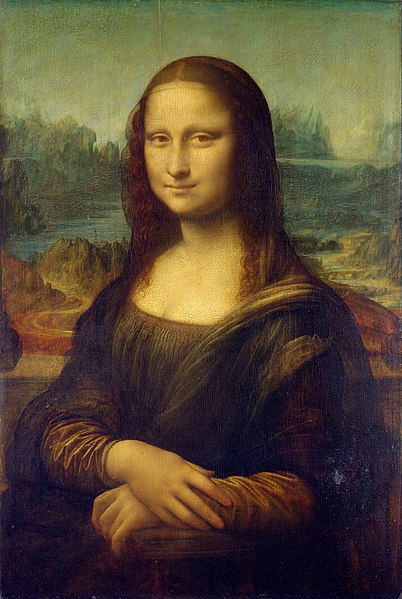
\includegraphics{monalisa}
	\caption[The Mona Lisa]{The Mona Lisa.\\ 
	\url{https://commons.wikimedia.org/wiki/File:Mona_Lisa,_by_Leonardo_da_Vinci,_from_C2RMF_retouched.jpg}}
	\labfig{marginmonalisa}
\end{marginfigure}

The order of the title pages, table of contents and preface can be 
easily changed, as in any \LaTeX\ document. In addition, the class is 
based on \KOMAScript's \Class{scrbook}, therefore it inherits all the 
goodies of that.

\section{What This Class Does Not Do}
\labsec{doesnot}

As anticipated, further customisation of the book is left to the user. 
Indeed, every book may have sidenotes, margin figures and so on, but 
each book will have its own fonts, toc style, special environments and 
so on. For this reason, in addition to the class, we provide only 
sensible defaults, but if these features are not needed, they can be 
left out. These special packages are located in the \Path{style} 
directory, which is organised as follows:

\begin{description}
	\item[kao.sty] This package contains the most important definitions 
	of macros and specifications of page layout. It is the heart of the 
	\Class{kaobook}.
	\item[kaobiblio.sty] Contains commands to add citations and 
	customise the bibliography.
	\item[packages.sty] Loads additional packages to decorate the 
	writing with special contents (for instance, the \Package{listing} 
	package is loaded here as it is not required in every book). There 
	are also defined some useful commands to print the same words always 
	in the same way, \eg latin words in italics or \Package{packages} in 
	verbatim.
	\item[kaorefs.sty] Some useful commands to manage labeling and 
	referencing, again to ensure that the same elements are referenced 
	always in a consistent way.
	\item[environments.sty] Provides special environments, like boxes. 
	Both simple and complex environments are available; by complex we 
	mean that they are endowed with a counter, floating and can be put 
	in a special table of contents.\sidenote[][-2mm]{See 
	\vrefch{mathematics} for some examples.}
	\item[theorems.sty] The style of mathematical environments. 
	Actually, there are two such packages: one is for plain theorems,
	\ie the theorems are printed in plain text; the other uses 
	\Package{mdframed} to draw a box around theorems. You can plug the 
	most appropriate style into its document.
\end{description}

\marginnote[2mm]{The audacious users might feel tempted to edit some of 
these packages. I'd be immensely happy if they sent me examples of what 
they have been able to do!}

In the rest of the book, I shall assume that the reader is not a novice 
in the use of \LaTeX, and refer to the documentation of the packages 
used in this class for things that are already explained there. 
Moreover, I assume that the reader is willing to make minor edits to the 
provided packages for styles, environments and commands, if he or she 
does not like the default settings.

\section{How to Use This Class}

Either if you are using the template from 
\href{http://latextemplates.org/template/kaobook}{latextemplates}, or if 
you cloned the GitHub 
\href{https://www.github.com/fmarotta/kaobook}{repository}, there are 
infinite ways to use the \Class{kaobook} class in practice, but we will 
discuss only two of them. The first is to find the \Path{main.tex} file 
which I used to write this book, and edit it; this will probably involve 
a lot of text-deleting, copying-and-pasting, and rewriting. The second 
way is to start almost from scratch and use the \Path{skeleton.tex} 
file, which is a cleaned-up version of the \Path{main.tex}; even if you 
choose the second way, you may find it useful to draw inspiration from 
the \Path{main.tex} file.

To compile the document, assuming that its name is \Path{main.tex}, you 
will have to run the following sequence of commands:

\begin{lstlisting}[style=kaolstplain,linewidth=1.5\textwidth]
pdflatex main # Compile template
makeindex main.nlo -s nomencl.ist -o main.nls # Compile nomenclature
makeindex main # Compile index
biber main # Compile bibliography
makeglossaries main # Compile glossary
pdflatex main # Compile template again
pdflatex main # Compile template again
\end{lstlisting}

You may need to compile the template some more times in order for some 
errors to disappear. For any support requests, please ask a question on 
\url{tex.stackexchange.org} with the tag \enquote{kaobook}, open an 
issue on GitHub, or contact the author via e-mail.


% \pagelayout{wide} % No margins
% \addpart{环境沙拉电话覅欧委会覅哦}
\pagelayout{margin} % Restore margins

\setchapterpreamble[u]{\margintoc}
\chapter{Class Options}
\labch{options}

In this chapter I will describe the most common options used, both the 
ones inherited from \Class{scrbook} and the \Class{kao}-specific ones. 
Options passed to the class modifies its default behaviour; beware 
though that some options may lead to unexpected results\ldots

\section{\Class{KOMA} Options}

The \Class{kaobook} class is based on \Class{scrbook}, therefore it 
understands all of the options you would normally pass to that class. If 
you have a lot of patience, you can read the \KOMAScript\xspace 
guide.\sidenote{The guide can be downloaded from 
\url{https://ctan.org/pkg/koma-script?lang=en}.} Actually, the reading 
of such guide is suggested as it is very instructive.

Every \KOMAScript\xspace option you pass to the class when you load it 
is automatically activated. In addition, in \Class{kaobook} some options 
have modified default values. For instance, the font size is 9.5pt and 
the paragraphs are separated by space,\sidenote[][-7mm]{To be precise, 
they are separated by half a line worth of space: the \Option{parskip} 
value is \enquote{half}.} not marked by indentation.

\section{\Class{kao} Options}

In the future I plan to add more options to set the paragraph formatting 
(justified or ragged) and the position of the margins (inner or outer in 
twoside mode, left or right in oneside mode).\sidenote{As of now, 
paragraphs are justified, formatted with \Command{singlespacing} (from 
the \Package{setspace} package) and \Command{frenchspacing}.}

I take this opportunity to renew the call for help: everyone is 
encouraged to add features or reimplement existing ones, and to send me 
the results. You can find the GitHub repository at 
\url{https://github.com/fmarotta/kaobook}.

\begin{kaobox}[frametitle=To Do]
Implement the \Option{justified} and \Option{margin} options. To be 
consistent with the \KOMAScript\xspace style, they should accept a 
simple switch as a parameter, where the simple switch should be 
\Option{true} or \Option{false}, or one of the other standard values for 
simple switches supported by \KOMAScript. See the \KOMAScript\xspace 
documentation for further information.
\end{kaobox}

The above box is an example of a \Environment{kaobox}, which will be 
discussed more thoroughly in \frefch{mathematics}. Throughout the book I 
shall use these boxes to remarks what still needs to be done.

\section{Other Things Worth Knowing}

A bunch of packages are already loaded in the class because they are 
needed for the implementation. These include:

\begin{itemize}
	\item etoolbox
	\item calc
	\item xifthen
	\item xkeyval
	\item xparse
	\item xstring
\end{itemize}

Many more packages are loaded, but they will be discussed in due time. 
Here, we will mention only one more set of packages, needed to change 
the paragraph formatting (recall that in the future there will be 
options to change this). In particular, the packages we load are:

\begin{itemize}
	\item ragged2e
	\item setspace
	\item hyphenat
	\item microtype
	\item needspace
	\item xspace
	\item xcolor (with options \Option{usenames,dvipsnames})
\end{itemize}

Some of the above packages do not concern paragraph formatting, but we 
nevertheless grouped them with the others. By default, the main text is 
justified and formatted with singlespacing and frenchspacing; the margin 
text is the same, except that the font is a bit smaller.

As a last warning, please be aware that the \Package{cleveref} package 
is not compatible with \Class{kaobook}. You should use the commands 
discussed in \refsec{hyprefs} instead.

\section{Document Structure}

We provide optional arguments to the \Command{title} and 
\Command{author} commands so that you can insert short, plain text 
versions of this fields, which can be used, typically in the half-title 
or somewhere else in the front matter, through the commands 
\Command{@plaintitle} and \Command{@plainauthor}, respectively. The PDF 
properties \Option{pdftitle} and \Option{pdfauthor} are automatically 
set by hyperref to the plain values if present, otherwise to the normal 
values.\sidenote[][*-1]{We think that this is an important point so 
we remark it here. If you compile the document with pdflatex, the PDF 
metadata will be altered so that they match the plain title and author 
you have specified; if you did not specify them, the metadata will be 
set to the normal title and author.}

There are defined two page layouts, \Option{margin} and \Option{wide}, 
and two page styles, \Option{plain} and \Option{fancy}. The layout 
basically concern the width of the margins, while the style refers to 
headers and footer; these issues will be 
discussed in \frefch{layout}.\sidenote[][6mm]{For now, suffice it to say that pages with 
the \Option{margin} layout have wide margins, while with the 
\Option{wide} layout the margins are absent. In \Option{plain} pages the 
headers and footer are suppressed, while in \Option{fancy} pages there 
is a header.} 

The commands \Command{frontmatter}, \Command{mainmatter}, and 
\Command{backmatter} have been redefined in order to automatically 
change page layout and style for these sections of the book. The front 
matter uses the \Option{margin} layout and the \Option{plain} page 
style. In the mainmatter the margins are wide and the headings are 
fancy. In the appendix the style and the layout do not change; however 
we use \Command{bookmarksetup\{startatroot\}} so that the bookmarks of 
the chapters are on the root level (without this, they would be under 
the preceding part). In the backmatter the margins shrink again and we 
also reset the bookmarks root.

\setchapterpreamble[u]{\margintoc}
\chapter{Margin Stuff}

Sidenotes are a distinctive feature of all 1.5-column-layout books. 
Indeed, having wide margins means that some material can be displayed 
there. We use margins for all kind of stuff: sidenotes, marginnotes, 
small tables of contents, citations, and, why not?, special boxes and 
environments.

\section{Sidenotes}

Sidenotes are like footnotes, except that they go in the margin, where 
they are more readable. To insert a sidenote, just use the command 
\Command{sidenote\{Text of the note\}}. You can specify a 
mark\sidenote[O]{This sidenote has a special mark, a big O!} with \\ 
\Command{sidenote[mark]\{Text\}}, but you can also specify an offset, 
which moves the sidenote upwards or downwards, so that the full syntax is:

\begin{lstlisting}[style=kaolstplain]
\sidenote[mark][offset]{Text}
\end{lstlisting}

If you use an offset, you always have to add the brackets for the mark, 
but they can be empty.\sidenote{If you want to know more about the usage 
of the \Command{sidenote} command, read the documentation of the 
\Package{sidenotes} package.}

In \Class{kaobook} we copied a feature from the \Package{snotez} 
package: the possibility to specify a multiple of \Command{baselineskip} 
as an offset. For example, if you want to enter a sidenote with the 
normal mark and move it upwards one line, type:

\begin{lstlisting}[style=kaolstplain]
\sidenote[][*-1]{Text of the sidenote.}
\end{lstlisting}

As we said, sidenotes are handled through the \Package{sidenotes} 
package, which in turn relies on the \Package{marginnote} package.

\section{Marginnotes}

This command is very similar to the previous one. You can create a 
marginnote with \Command{marginnote[offset]\{Text\}}, where the offset 
argument can be left out, or it can be a multiple of 
\Command{baselineskip},\marginnote[-1cm]{While the command for margin 
notes comes from the \Package{marginnote} package, it has been redefined 
in order to change the position of the optional offset argument, which 
now precedes the text of the note, whereas in the original version it 
was at the end. We have also added the possibility to use a multiple of 
\Command{baselineskip} as offset. These things were made only to make 
everything more consistent, so that you have to remember less things!} 
\eg

\begin{lstlisting}[style=kaolstplain]
\marginnote[-12pt]{Text} or \marginnote[*-3]{Text}
\end{lstlisting}

\begin{kaobox}[frametitle=To Do]
A small thing that needs to be done is to renew the \Command{sidenote} 
command so that it takes only one optional argument, the offset. The 
special mark argument can go somewhere else. In other words, we want the 
syntax of \Command{sidenote} to resemble that of \Command{marginnote}.
\end{kaobox}

We load the packages \Package{marginnote}, \Package{marginfix} and 
\Package{placeins}. Since \Package{sidenotes} uses \Package{marginnote}, 
what we said for marginnotes is also valid for sidenotes. Side- and 
margin- notes are shifted slightly upwards 
(\Command{renewcommand\{\textbackslash marginnotevadjust\}\{3pt\}}) in 
order to align them to the bottom of the line of text where the note is 
issued. Importantly, both sidenotes and marginnotes are defined as 
floating if the optional argument (\ie the vertical offset) is left 
blank, but if the offset is specified they are not floating. Recall that 
floats cannot be nested, so in some rare cases you may encounter errors 
about lost floats; in those cases, remember that sidenotes and 
marginnotes are floats. To solve the problem, it may be possible to 
transform them into non-floating elements by specifying an offset of 
0pt.

\section{Footnotes}

Even though they are not displayed in the margin, we will discuss about 
footnotes here, since sidenotes are mainly intended to be a replacement 
of them. Footnotes force the reader to constantly move from one area of 
the page to the other. Arguably, marginnotes solve this issue, so you 
should not use footnotes. Nevertheless, for completeness, we have left 
the standard command \Command{footnote}, just in case you want to put a 
footnote once in a while.\footnote{And this is how they look like. 
Notice that in the PDF file there is a back reference to the text; 
pretty cool, uh?}

\section{Margintoc}

Since we are talking about margins, we introduce here the 
\Command{margintoc} command, which allows one to put small table of 
contents in the margin. Like other commands we have discussed, 
\Command{margintoc} accepts a parameter for the vertical offset, like 
so: \Command{margintoc[offset]}.

The command can be used in any point of the document, but we think it 
makes sense to use it just at the beginning of chapters or parts. In 
this document I make use of a \KOMAScript\xspace feature and put it in 
the chapter preamble, with the following code:

\marginnote{The font used in the margintoc is the same as the one for 
	the chapter entries in the main table of contents at the beginning 
	of the document.}

\begin{lstlisting}[style=kaolstplain]
\setchapterpreamble[u]{\margintoc}
\chapter{Chapter title}
\end{lstlisting}

\section{Marginlisting}

On some occasions it may happen that you have a very short piece of code 
that doesn't look good in the body of the text because it breaks the 
flow of narration: for that occasions, you can use a 
\Environment{marginlisting}. The support for this feature is still 
limited, especially for the captions, but you can try the following 
code:

\begin{marginlisting}[-1.35cm]
	\caption{An example of a margin listing.}
	\vspace{0.6cm}
	\begin{lstlisting}[language=Python,style=kaolstplain]
print("Hello World!")
	\end{lstlisting}
\end{marginlisting}

\begin{verbatim}
\begin{marginlisting}[-0.5cm]
	\caption{My caption}
	\vspace{0.2cm}
	\begin{lstlisting}[language=Python,style=kaolstplain]
	... code ...
	\end{lstlisting}
\end{marginlisting}
\end{verbatim}

Unfortunately, the space between the caption and the listing must be 
adjusted manually; if you find a better way, please let me know.

Not only textual stuff can be displayed in the margin, but also figures. 
Those will be the focus of the next chapter.

\setchapterimage[6.5cm]{seaside}
\setchapterpreamble[u]{\margintoc}
\chapter[Figures and Tables]{Figures and Tables\footnotemark[0]}

\footnotetext{The credits for the image above the chapter title go to:
	Bushra Feroz, CC~BY-SA~4.0, \url{https://commons.wikimedia.org/w/index.php?curid=68724647}}

\section{Normal Figures and Tables}

Figures and tables can be inserted just like in any standard 
\LaTeX\xspace document. The \Package{graphicx} package is already loaded 
and configured in such a way that the figure width is equal to the 
textwidth and the height is adjusted in order to maintain the original 
aspect ratio. As you may have imagined, the captions will be 
positioned\ldots well, in the margins. This is achieved with the help of 
the \Package{floatrow} package.

Here is a picture of Mona Lisa (\reffig{normalmonalisa}), as an example. 
The captions are formatted as the margin- and the side-notes; If you 
want to change something about captions you can use the command 
\Command{captsetup} from the \Package{caption} package. Remember that if 
you want to reference a figure, the label must come \emph{after} the 
caption!

\begin{figure}[hb]
	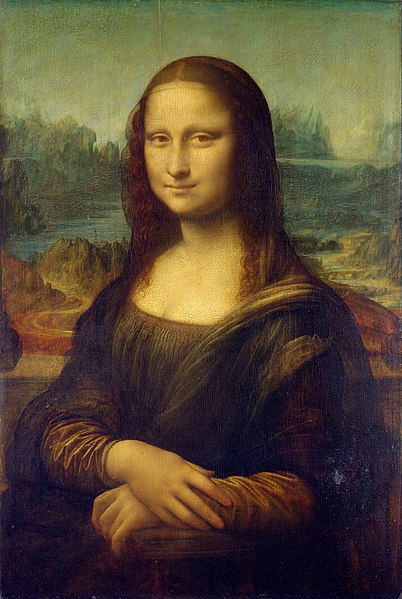
\includegraphics[width=0.45\textwidth]{monalisa}
	\caption[Mona Lisa, again]{It's Mona Lisa again. \blindtext}
	\labfig{normalmonalisa}
\end{figure}

While the format of the caption is managed by \Package{caption}, its 
position is handled by the \Package{floatrow} package. Achieving this 
result has been quite hard, but now I am pretty satisfied. In two-side 
mode, the captions are printed in the correct margin.

Tables can be inserted just as easily as figures, as exemplified by the 
following code:

\begin{lstlisting}[caption={Caption of a listing.}]
\begin{table}
\begin{tabular}{ c c c c }
	\toprule
	col1 & col2 & col3 & col 4 \\
	\midrule
	\multirow{3}{4em}{Multiple row} & cell2 & cell3 & cell4\\ &
	cell5 & cell6 & cell7 \\ &
	cell8 & cell9 & cell10 \\
	\multirow{3}{4em}{Multiple row} & cell2 & cell3 & cell4 \\ &
	cell5 & cell6 & cell7 \\ &
	cell8 & cell9 & cell10 \\
	\bottomrule
\end{tabular}
\end{table}
\end{lstlisting}

which results in the useless \vreftab{useless}.

\begin{table}[h]
\caption[A useless table]{A useless table.}
\labtab{useless}
\begin{tabular}{ c c c c }
	\toprule
	col1 & col2 & col3 & col 4 \\
	\midrule
	\multirow{3}{4em}{Multiple row} & cell2 & cell3 & cell4\\ &
	cell5 & cell6 & cell7 \\ &
	cell8 & cell9 & cell10 \\
	\multirow{3}{4em}{Multiple row} & cell2 & cell3 & cell4 \\ &
	cell5 & cell6 & cell7 \\ &
	cell8 & cell9 & cell10 \\
	\bottomrule
\end{tabular}
\end{table}

I don't have much else to say, so I will just insert some blind text. 
\blindtext

\section{Margin Figures and Tables}

Marginfigures can be inserted with the environment 
\Environment{marginfigure}. In this case, the whole picture is confined 
to the margin and the caption is below it. \reffig{marginmonalisa} is 
obtained with something like this:

\begin{lstlisting}[caption={Another caption.}]
\begin{marginfigure}
	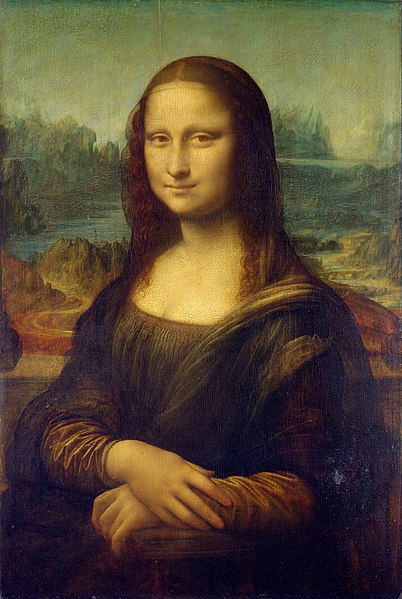
\includegraphics{monalisa}
	\caption[The Mona Lisa]{The Mona Lisa.}
	\labfig{marginmonalisa}
\end{marginfigure}
\end{lstlisting}

There is also the \Environment{margintable} environment, of which 
\reftab{anotheruseless} is an example. Notice how you can place the 
caption above the table by just placing the \Command{caption} command 
before beginning the \Environment{tabular} environment. Usually, figure 
captions are below, while table captions are above. This rule is also 
respected for normal figures and tables: the captions are always on the 
side, but for figure they are aligned to the bottom, while for tables to 
the top.

\begin{margintable}
\caption[Another useless table]{Another useless table.}
\labtab{anotheruseless}
\raggedright
\begin{tabular}{ c c c c }
	\hline
	col1 & col2 & col3 \\
	\hline
	\multirow{3}{4em}{Multiple row} & cell2 & cell3 \\ & cell5 & cell6 
	\\ & cell8 & cell9 \\ \hline
\end{tabular}
\end{margintable}

Marginfigures and tables can be positioned with an optional offset 
command, like so:

\begin{lstlisting}
\begin{marginfigure}[offset]
	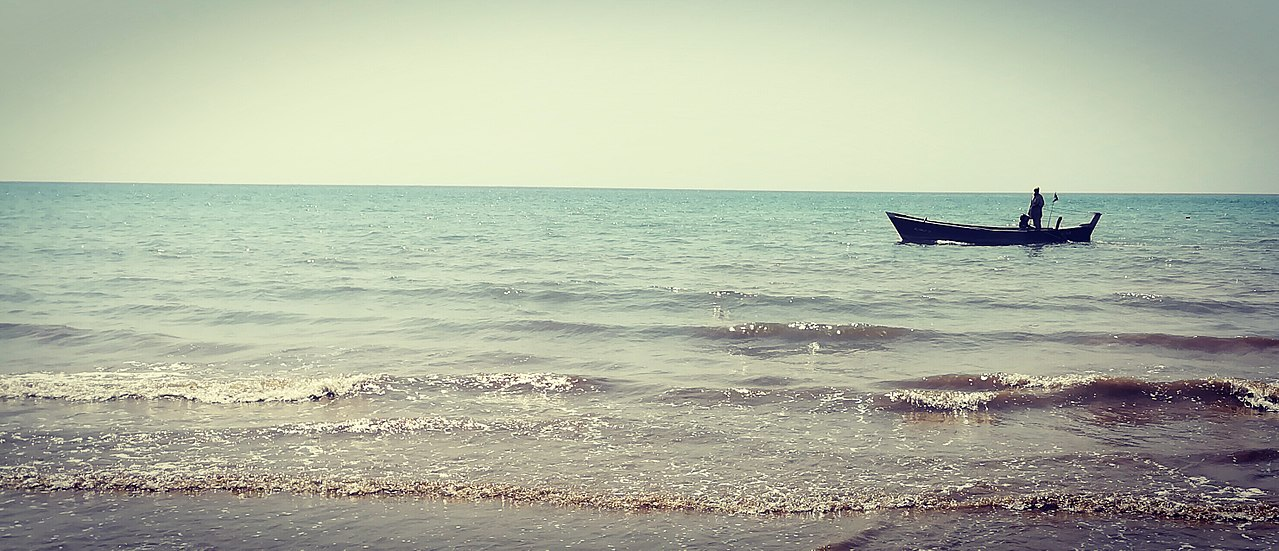
\includegraphics{seaside}
\end{marginfigure}
\end{lstlisting}

Offset ca be either a measure or a multiple of \Command{baselineskip}, 
much like with \Command{sidenote}, \Command{marginnote} and 
\Command{margintoc}.\todo{Improve this part.} If you are wondering how I 
inserted this orange bubble, have a look at the \Package{todo} package.

\section{Wide Figures and Tables}

With the environments \Environment{figure*} and \Environment{table*} you 
can insert figures which span the whole page width. For example, here 
are a wide figure and a wide table.

\begin{figure*}[h!]
	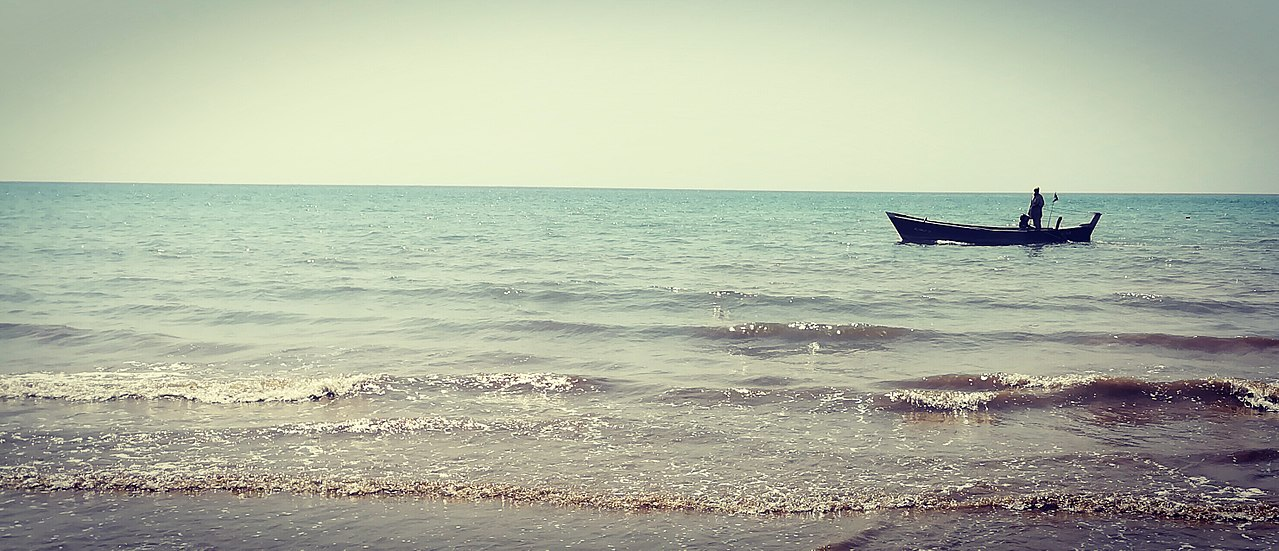
\includegraphics{seaside}
	\caption[A wide seaside]{A wide seaside, and a wide caption.
		Credits: By Bushra Feroz, CC BY-SA 4.0, \url{https://commons.wikimedia.org/w/index.php?curid=68724647}}
\end{figure*}

\begin{table*}[h!]
    \caption{A wide table with invented data about three people living in the UK. Note that wide figures and tables are centered and their caption also extends into the margin.}
    \begin{tabular}{p{2.0cm} p{2.0cm} p{2.0cm} p{2.0cm} p{2.0cm} p{2.0cm} p{1.5cm}}
        \toprule
        Name    & Surname   & Job       & Salary           & Age   & Height    & Country \\
        \midrule
        Alice   & Red       & Writer    & 4.000 \pounds    & 34    & 167 cm     & England \\
        Bob     & White     & Bartender & 2.000 \pounds    & 24    & 180 cm     & Scotland \\
        Drake   & Green     & Scientist & 4.000 \pounds    & 26    & 175 cm     & Wales \\
        \bottomrule
    \end{tabular}
\end{table*}

It is the user's responsibility to adjust the width of the table, if 
necessary, until it is aesthetically pleasing. The previous table was 
obtained with the following code:

\begin{lstlisting}[caption=How to typeset a wide table]
\begin{table*}[h!]
    \caption{A wide table with invented data about three people living in the UK. Note that wide figures and tables are centered and their caption also extends into the margin.}
    \begin{tabular}{p{2.0cm} p{2.0cm} p{2.0cm} p{2.0cm} p{2.0cm} p{2.0cm} p{1.5cm}}
        \toprule
        Name    & Surname   & Job       & Salary           & Age   & Height    & Country \\
        \midrule
        Alice   & Red       & Writer    & 4.000 \pounds    & 34    & 167 cm     & England \\
        Bob     & White     & Bartender & 2.000 \pounds    & 24    & 180 cm     & Scotland \\
        Drake   & Green     & Scientist & 4.000 \pounds    & 26    & 175 cm     & Wales \\
        \bottomrule
    \end{tabular}
\end{table*}
\end{lstlisting}

You may have noticed the full width image at the very beginning of this
chapter: that, however, is set up in an entirely different way, which
you'll read about in \vrefch{layout}.

\Class{kaobook} also supports paginated tables (have a look at the 
\Package{longtable} package). The 
\Environment{longtable}\sidenote{Interestingly, \Environment{longtable}s 
may require up to four rounds of compilation before they are typeset 
correctly.} environment behaves a bit differently from 
\Environment{table}, in that \Environment{longtable} encompasses both 
\Environment{table} and \Environment{tabular}, so that you can write, 
\eg,

\begin{lstlisting}[caption=Example of a longtable]
\begin{longtable}{|l c c|}
    \hline
    One & Two & Three \\
    Left & Center & Center \\
    \hline
    \caption{Caption of the longtable.}
\end{longtable}
\end{lstlisting}

to obtain the following table:
\begin{longtable}{|l c c|}
    \hline
    One & Two & Three \\
    Left & Center & Center \\
    \hline
    \caption{Caption of the longtable.}
\end{longtable}

The caption of a \Environment{longtable} is always positioned below the 
table, and it has the same width as the text (it doesn't extend into the 
margin). However, sometimes you may need a \Environment{longtable} that 
is so wide that it trespass into the margins; in those cases, you may 
want to also increase the width of the caption. To do so, you'll have to 
write two additional commands, one before and one after the 
\Environment{longtable}:

\begin{lstlisting}[caption=Increasing the width of the caption of a \Environment{longtable}.]
\floatsetup[longtable]{margins=centering,LTcapwidth=table} % Add this line before the longtable to increase the caption width
\begin{longtable}{lp{8cm}p{5cm}p{2cm}}
...
\end{longtable}
\floatsetup[longtable]{margins=raggedright,LTcapwidth=\textwidth} % Add this line after the longtable to revert the previous change
\end{lstlisting}

Having seen figures and tables, it is now time to tackle 
hyperreferences.

\setchapterstyle{kao}
%\setchapterpreamble[u]{\margintoc}
\chapter{References}
\labch{references}

\section{Citations}

\index{citations}
To cite someone \sidecite{Visscher2008,James2013} is very simple: just 
use the \Command{sidecite}\index{\Command{sidecite}} command. It does 
not have an offset argument yet, but it probably will in the future. 
This command supports multiple entries, as you can see, and by default 
it prints the reference on the margin as well as adding it to the 
bibliography at the end of the document. Note that the citations have 
nothing to do with the text,\sidecite{James2013} but they are completely 
random as they only serve the purpose to illustrate the feature.

For this setup I wrote a separate package, \Package{kaobiblio}, which 
you can find in the \Package{styles} directory and include in your main 
tex file. This package accepts all the options that you can pass to 
\Package{biblatex}, and actually it passes them to \Package{biblatex} 
under the hood. Moreover, it also defines some commands, like 
\Command{sidecite}, and environments that can be used within a 
\Class{kao} book.\sidenote{For this reason you should always use 
\Package{kaobiblio} instead of \Package{biblatex}, but the syntax and 
the options are exactly the same.}

If you want to use \Package{bibtex} instead of \Package{biblatex}, pass 
the option \Option{backend=bibtex} to \Package{kaobiblio}.

As you have seen, the \Command{sidecite} command will print a citation 
in the margin. However, this command would be useless without a way to 
customise the format of the citation, so the \Class{kaobook} provides 
also the \Command{formatmargincitation} command. By \enquote{renewing} 
that command, you can choose which items will be printed in the margins. 
The best way to understand how it works is to see the actual definition 
of this command.

\begin{lstlisting}[style=kaolstplain,linewidth=1.5\textwidth]
\newcommand{\formatmargincitation}[1]{%
	\parencite{#1}: \citeauthor*{#1} (\citeyear{#1}), \citetitle{#1}%
}
\end{lstlisting}

Thus, the \Command{formatmargincitation} accepts one parameter, which is 
the citation key, and prints the parencite followed by a colon, then the 
author, then the year (in brackets), and finally the 
title.\sidecite{Battle2014} Now, suppose that you wish the margin 
citation to display the year and the author, followed by the title, and 
finally a fixed arbitrary string; you would add to your document:

\begin{lstlisting}[style=kaolstplain,linewidth=1.5\textwidth]
\renewcommand{\formatmargincitation}[1]{%
	\citeyear{#1}, \citeauthor*{#1}: \citetitle{#1}; very interesting!%
}
\end{lstlisting}

\renewcommand{\formatmargincitation}[1]{%
	\citeyear{#1}, \citeauthor*{#1}: \citetitle{#1}; very interesting!%
}

The above code results in citations that look like the 
following.\sidecite{Zou2005} Of course, changing the format is most 
useful when you also change the default bibliography style. For 
instance, if you want to use the \enquote{philosophy-modern} style for 
your bibliography, you might have something like this in the preamble:

\begin{lstlisting}[style=kaolstplain,linewidth=1.5\textwidth]
\usepackage[style=philosophy-modern]{styles/kaobiblio}
\renewcommand{\formatmargincitation}[1]{%
	\sdcite{#1}%
}
\addbibresource{main.bib}
\end{lstlisting}

\renewcommand{\formatmargincitation}[1]{%
	\parencite{#1}: \citeauthor*{#1} (\citeyear{#1}), \citetitle{#1}%
}

The commands like \Command{citeyear}, \Command{parencite}
and \Command{sdcite} are just examples. A full
reference of the available commands can be found in this
\href{http://tug.ctan.org/info/biblatex-cheatsheet/biblatex-cheatsheet.pdf}{cheatsheet},
under the \enquote{Citations} section.

Finally, to compile a document containing citations, you need to use an 
external tool, which for this class is biber. You need to run the 
following (assuming that your tex file is called main.tex):

\begin{lstlisting}[style=kaolstplain]
$ pdflatex main
$ biber main
$ pdflatex main
\end{lstlisting}

\section{Glossaries and Indices}

\index{glossary}
The \Class{kaobook} class loads the packages \Package{glossaries} and 
\Package{imakeidx}, with which you can add glossaries and indices to 
your book. For instance, I previously defined some glossary entries and 
now I am going to use them, like this: \gls{computer}. 
\Package{glossaries} also allows you to use acronyms, like the 
following: this is the full version, \acrfull{fpsLabel}, and this is the 
short one \acrshort{fpsLabel}. These entries will appear in the glossary 
in the backmatter.

Unless you use \href{https://www.overleaf.com}{Overleaf} or some other 
fancy IDE for \LaTeX, you need to run an external command from your 
terminal in order to compile a document with a glossary. In particular, 
the commands required are:\sidenote{These are the commands you would run 
in a UNIX system, but see also \nrefsec{compiling}; I have no idea about 
how it works in Windows.}

\begin{lstlisting}[style=kaolstplain]
$ pdflatex main
$ makeglossaries main
$ pdflatex main
\end{lstlisting}

Note that you need not run \texttt{makeglossaries} every time you 
compile your document, but only when you change the glossary entries.

\index{index}
To create an index, you need to insert the command 
\lstinline|\index{subject}| whenever you are talking about 
\enquote{subject} in the text. For instance, at the start of this 
paragraph I would write \lstinline|index{index}|, and an entry would be 
added to the Index in the backmatter. Check it out!

\marginnote[2mm]{In theory, you would need to run an external command 
for the index as well, but luckily the package we suggested, 
	\Package{imakeidx}, can compile the index automatically.}

\index{nomenclature}
A nomenclature is just a special kind of index; you can find one at the end of
this book. To insert a nomenclature, we use the package \Package{nomencl} and
add the terms with the command \Command{nomenclature}. We put then a
\Command{printnomenclature} where we want it to appear.

Also with this package we need to run an external command to compile the 
document, otherwise the nomenclature will not appear:

\begin{lstlisting}[style=kaolstplain]
$ pdflatex main
$ makeindex main.nlo -s nomencl.ist -o main.nls
$ pdflatex main
\end{lstlisting}

These packages are all loaded in 
\href{style/packages.sty}{packages.sty}, one of the files that come with 
this class. However, the configuration of the elements is best done in 
the main.tex file, since each book will have different entries and 
styles.

Note that the \Package{nomencl} package caused problems when the 
document was compiled, so, to make a long story short, I had to prevent 
\Package{scrhack} to load the hack-file for \Package{nomencl}. When 
compiling the document on Overleaf, however, this problem seem to 
vanish.

\marginnote[-19mm]{This brief section was by no means a complete 
reference on the subject, therefore you should consult the documentation 
of the above package to gain a full understanding of how they work.}

\section{Hyperreferences}
\labsec{hyprefs}

\index{hyperreferences}
Together with this class we provide a handy package to help you 
referencing the same elements always in the same way, for consistency 
across the book. First, you can label each element with a specific 
command. For instance, should you want to label a chapter, you would put 
\lstinline|\labch{chapter-title}| right after the \Command{chapter} 
directive. This is just a convenience, because \Command{labch} is
actually just an alias to \lstinline|\label{ch:chapter-title}|, so it 
spares you the writing of \enquote{ch:}. We defined similar commands for 
many typically labeled elements, including:

\begin{multicols}{2}
\setlength{\columnseprule}{0pt}
\begin{itemize}
	\item Page: \Command{labpage}
	\item Part: \Command{labpart}
	\item Chapter: \Command{labch}
	\item Section: \Command{labsec}
	\item Figure: \Command{labfig}
	\item Table: \Command{labtab}
	\item Definition: \Command{labdef}
	\item Assumption: \Command{labassum}
	\item Theorem: \Command{labthm}
	\item Proposition: \Command{labprop}
	\item Lemma: \Command{lablemma}
	\item Remark: \Command{labremark}
	\item Example: \Command{labexample}
	\item Exercise: \Command{labexercise}
\end{itemize}
\end{multicols}

Of course, we have similar commands for referencing those elements. 
However, since the style of the reference should depend on the context, 
we provide different commands to reference the same thing. For instance, 
in some occasions you may want to reference the chapter by name, but 
other times you want to reference it only by number. In general, there 
are four reference style, which we call plain, vario, name, and full.

The plain style references only by number. It is accessed, for chapters, 
with \lstinline|\refch{chapter-title}| (for other elements, the syntax 
is analogous). Such a reference results in: \refch{references}.

The vario and name styles rest upon the \Package{varioref} package. 
Their syntax is \lstinline|\vrefch{chapter-title}| and 
\lstinline|\nrefch{chapter-title}|, and they result in: 
\vrefch{references}, for the vario style, and: \nrefch{references}, for 
the name style. As you can see, the page is referenced in 
\Package{varioref} style.

The full style references everything. You can use it with 
\lstinline|\frefch{chapter-title}| and it looks like this: 
\frefch{references}.

Of course, all the other elements have similar commands (\eg for parts 
you would use \lstinline|\vrefpart{part-title}| or something like that). 
However, not all elements implement all the four styles. The commands 
provided should be enough, but if you want to see what is available or 
to add the missing ones, have a look at the 
\href{styles/kaorefs.sty}{attached package}.

In order to have access to all these features, the \Package{kaorefs} 
should be loaded in the preamble of your document. It should be loaded 
last, or at least after \Package{babel} (or \Package{polyglossia}) and 
\Package{plaintheorems} (or \Package{mdftheorems}). Options can be 
passed to it like to any other package; in particular, it is possible to 
specify the language of the captions. For instance, if you specify 
\enquote{italian} as an option, instead of \enquote{Chapter} it will be 
printed \enquote{Capitolo}, the Italian analog. If you know other 
languages, you are welcome to contribute the translations of these 
captions! Feel free to contact the author of the class for further 
details. 

The \Package{kaorefs} package also include \Package{cleveref}, so it is 
possible to use \Command{cref} in addition to all the previously 
described referencing commands.

\section{A Final Note on Compilation}
\labsec{compiling}

Probably the easiest way to compile a latex document is with the 
\Package{latexmk} script, as it can take care of everything, if properly 
configured, from the bibliography to the glossary. The command to issue, 
in general, is:

\begin{lstlisting}
latexmk [latexmk_options] [filename ...]
\end{lstlisting}

\Package{latexmk} can be extensively configured (see
\url{https://mg.readthedocs.io/latexmk.html}). For convenience, I print 
here an example configuration that would cover all the steps described 
above.

\begin{lstlisting}
# By default compile only the file called 'main.tex'
@default_files = ('main.tex');

# Compile the glossary and acronyms list (package 'glossaries')
add_cus_dep( 'acn', 'acr', 0, 'makeglossaries' );
add_cus_dep( 'glo', 'gls', 0, 'makeglossaries' );
$clean_ext .= " acr acn alg glo gls glg";
sub makeglossaries {
   my ($base_name, $path) = fileparse( $_[0] );
   pushd $path;
   my $return = system "makeglossaries", $base_name;
   popd;
   return $return;
}

# Compile the nomenclature (package 'nomencl')
add_cus_dep( 'nlo', 'nls', 0, 'makenlo2nls' );
sub makenlo2nls {
    system( "makeindex -s nomencl.ist -o \"$_[0].nls\" \"$_[0].nlo\"" );
}
\end{lstlisting}

However, if you'd rather not use an external package and want to do 
everything manually, here are some tips.\sidenote{As the author only 
uses Linux and compiles everything from the command line, he doesn't 
know how the compilation works in Windows or Mac. The tips, therefore, 
refer to the usage with Linux from the command line.}

\minisec{Compiling the examples in the kaobook repository}
To compile the examples, and in particular the documentation, that are 
in the \Path{examples} directory of the 
\href{https://github.com/fmarotta/kaobook}{kaobook repository} on 
GitHub, do as follows. \lstinline[language=bash]|cd| into the root 
directory of the repository, and run
\lstinline|pdflatex -output-directory examples/documentation main.tex|. 
With this trick, you can compile the documentation using the class files 
pertaining to the repository (and not, say, those in your texmf tree). 
The \enquote{-output-directory} option works with the other 
\LaTeX-related commands such as biber and makeglossaries.

A note of warning: sometimes \LaTeX\ needs more than one run to get the
correct position of each element; this is true in particular for the
positioning of floating elements like figures, tables, and margin notes.
Occasionally, \LaTeX\ can need up to four re-runs, so If the alignment
of margin elements looks odd, or if they bleed into ther main text, try
runnign pdflatex one more time.


\pagelayout{wide} % No margins
\addpart{Design and Additional Features}
\pagelayout{margin} % Restore margins

\setchapterimage[6cm]{seaside}
\setchapterpreamble[u]{\margintoc}
\chapter{Page Design}
\labch{layout}

\section{Headings}

So far, in this document I used two different styles for the chapter 
headings: one has the chapter name, a rule and, in the margin, the 
chapter number; the other has an image at the top of the page, and the 
chapter title is printed in a box (like for this chapter). There is one 
additional style, which I used only in the appendix 
(\vrefpage{appendix}); there, the chapter title is enclosed in two 
horizontal rules, and the chapter number (or letter, in the case of the 
appendix) is above it.\sidenote{To be honest, I do not think that mixing 
heading styles like this is a wise choice, but in this document I did it 
only to show you how they look.}

Every book is unique, so it makes sense to have different styles from 
which to choose. Actually, it would be awesome if whenever a 
\Class{kao}-user designs a new heading style, he or she added it to the 
three styles already present, so that it will be available for new users 
and new books.

The choice of the style is made simple by the \Command{setchapterstyle} 
command. It accepts one option, the name of the style, which can be: 
\enquote{plain}, \enquote{kao}, or \enquote{lines}.\sidenote{Plain is 
the default \LaTeX\xspace title style; the other ones are self 
explanatory.} If instead you want the image style, you have to use the 
command \Command{setchapterimage}, which accepts the path to the image 
as argument; you can also provide an optional parameter in square 
brackets to specify the height of the image.

Let us make some examples. In this book, I begin a normal chapter with 
the lines:

\begin{lstlisting}
\setchapterstyle{kao}
\setchapterpreamble[u]{\margintoc}
\chapter{Title of the Chapter}
\labch{title}
\end{lstlisting}

In Line 1 I choose the style for the title to be \enquote{kao}. Then, I 
specify that I want the margin toc. The rest is ordinary administration 
in \LaTeX, except that I use my own \Command{labch} to label the 
chapter. Actually, the \Command{setchapterpreamble} is a standard 
\KOMAScript\xspace one, so I invite you to read about it in the KOMA
documentation. Once the chapter style is set, it holds until you change 
it.\sidenote{The \Command{margintoc} has to be specified at every 
chapter. Perhaps in the future this may change; it all depends on how 
this feature will be welcomed by the users, so keep in touch with me if 
you have preferences!} Whenever I want to start a chapter with an image, 
I simply write:

\begin{lstlisting}
\setchapterimage[7cm]{path/to/image.png} % Optionally specify the height
\setchapterpreamble[u]{\margintoc}
\chapter{Catchy Title} % No need to set a chapter style
\labch{catchy}
\end{lstlisting}

If you prefer, you can also specify the style at the beginning of the 
main document, and that style will hold until you change it again.

\section{Headers \& Footers}

Headers and footers in \KOMAScript\xspace are handled by the 
\Package{scrlayer-scrpage} package. There are two basic style: 
\enquote{scrheadings} and \enquote{plain.scrheadings}. The former is 
used for normal pages, whereas the latter is used in title pages (those 
where a new chapter starts, for instance) and, at least in this book, in 
the front matter. At any rate, the style can be changed with the 
\Command{pagestyle} command, \eg 
\lstinline|\pagestyle{plain.scrheadings}|.

In both styles, the footer is completely empty. In plain.scrheadings,
also the header is absent (otherwise it wouldn't be so plain\ldots), but 
in the normal style the design is reminiscent of the \enquote{kao} style
for chapter titles.

\begin{kaobox}[frametitle=To Do]
The \Option{twoside} class option is still unstable and may lead to 
unexpected behaviours. As always, any help will be greatly appreciated.
\end{kaobox}

\section{Table of Contents}

Another important part of a book is the table of contents. By default, 
in \Class{kaobook} there is an entry for everything: list of figures, 
list of tables, bibliographies, and even the table of contents itself. 
Not everybody might like this, so we will provide a description of the 
changes you need to do in order to enable or disable each of these 
entries. In the following \reftab{tocentries}, each item corresponds to 
a possible entry in the \acrshort{tocLabel}, and its description is the 
command you need to provide to have such entry. These commands are 
specified in the attached \href{style/style.sty}{style 
package},\sidenote{In the same file, you can also choose the titles of 
these entries.} so if you don't want the entries, just comment the 
corresponding lines.

Of course, some packages, like those for glossaries and indices, will 
try to add their own entries.\marginnote{In a later section, we will see 
how you can define your own floating environment, and endow it with an 
entry in the \acrshort{tocLabel}.} In such cases, you have to follow the 
instructions specific to that package. Here, since we have talked about 
glossaries and notations in \refch{references}, we will briefly see how
to configure them.

\begin{table}
\footnotesize
\caption{Commands to add a particular entry to the table of contents.}
\labtab{tocentries}
\begin{tabular}{ l l }
	\toprule
	Entry & Command to Activate \\
	\midrule
	Table of Contents & \lstinline|\setuptoc{toc}{totoc}| \\
	List of Figs and Tabs & \lstinline|\PassOptionsToClass{toc=listof}{\@baseclass}| \\
	Bibliography & \lstinline|\PassOptionsToClass{toc=bibliography}{\@baseclass}| \\
	\bottomrule
\end{tabular}
\end{table}

For the \Package{glossaries} package, use the \enquote{toc} option when 
you load it: \lstinline|\usepackage[toc]{glossaries}|. For 
\Package{nomencl}, pass the \enquote{intoc} option at the moment of 
loading the package. Both \Package{glossaries} and \Package{nomencl} are 
loaded in the attached \href{style/packages.sty}{\enquote{packages} 
package}.

Additional configuration of the table of contents can be performed 
through the packages \Package{etoc}, which is loaded because it is 
needed for the margintocs, or the more traditional \Package{tocbase}. 
Read the respective documentations if you want to be able to change the 
default \acrshort{tocLabel} style.\sidenote[][*-1]{(And please, send me 
a copy of what you have done, I'm so curious!)}

\section{Paper Size}

Recent versions of Kaobook support paper sizes different from the
default A4. It is possible to pass the name of the paper as an option
to the class, as we are accustomed for any other \LaTeX\ class. For
example, the class option \Option{b5paper} would set the paper size
to the B5 format.

We also support the paper sizes specified in
\href{https://www.bod.de/hilfe/hilfe-und-service.html?cmd=SINGLE\&entryID=2494\_GER\_WSS\&eo=2\&title=welche-buchformate-gibt-es}{this
web page} and some additional sizes requested by the users, with the 
option names specified in \reftab{papersizes}.

\begin{margintable}[*-6]
	\caption{Some non-standard paper sizes supported by kaobook.}
	\labtab{papersizes}
	\begin{tabular}{ll}
		\toprule
		Dimension & Option name \\
		\midrule
		12.0cm x 19.0cm & smallpocketpaper \\
		13.5cm x 21.5cm & pocketpaper \\
		14.8cm x 21.0cm & a5paper \\
		15.5cm x 22.0cm & juvenilepaper \\
		17.0cm x 17.0cm & smallphotopaper \\
		21.0cm x 15.0cm & appendixpaper \\
		17.0cm x 22.0cm & cookpaper \\
		19.0cm x 27.0cm & illustratedpaper \\
		17.0cm x 17.0cm & photopaper \\
		16.0cm x 24.0cm & f24paper \\
		%21.0cm x 29.7cm & a4paper \\
		\bottomrule
	\end{tabular}
\end{margintable}

For instance, to use the \enquote{smallpocketpaper} add the correct 
description at the beginning of the documentclass instruction:
\begin{lstlisting}
\documentclass[
		smallpocketpaper,
		fontsize=10pt,
		twoside=false,
		%open=any,
		secnumdepth=1,
]{kaobook}
\end{lstlisting}

\section{Page Layout}

Besides the page style, you can also change the width of the content of 
a page. This is particularly useful for pages dedicated to part titles, 
where having the 1.5-column layout might be a little awkward, or for 
pages where you only put figures, where it is important to exploit all 
the available space.

In practice, there are two layouts: \enquote{wide} and \enquote{margin}. 
The former suppresses the margins and allocates the full page for 
contents, while the latter is the layout used in most of the pages of 
this book, including this one. The wide layout is also used 
automatically in the front and back matters.

\marginnote{Sometimes it is desirable to increase the width for just one 
or a few paragraphs; the \Environment{widepar} environment does that: 
wrap your paragraphs in this environment, and they will occupy the full 
width of the page.}

To change page layout, use the \Command{pagelayout} command. For 
example, when I start a new part, I write:

\begin{lstlisting}
\pagelayout{wide}
\addpart{Title of the New Part}
\pagelayout{margin}
\end{lstlisting}

Beyond these two basic layouts, it is also possible to finely tune the 
page layout by redefining the \Command{marginlayout} command. This 
command is called internally by the higher-level \Command{pagelayout}, 
and it is responsible for setting the width of the margins and of the 
text. The default definition is:

\begin{lstlisting}
\newcommand{\marginlayout}{%
	\newgeometry{
		top=27.4mm,				% height of the top margin
		bottom=27.4mm,			% height of the bottom margin
		inner=24.8mm,			% width of the inner margin
		textwidth=107mm,		% width of the text
		marginparsep=8.2mm,		% width between text and margin
		marginparwidth=49.4mm,	% width of the margin
	}%
}
\end{lstlisting}

so if you want to, say, decrease the width of the margin while 
increasing the width of the text, you could write in the preamble of 
your document something like:

\begin{lstlisting}
\renewcommand{\marginlayout}{%
	\newgeometry{
		top=27.4mm,				% height of the top margin
		bottom=27.4mm,			% height of the bottom margin
		inner=24.8mm,			% width of the inner margin
		textwidth=117mm,		% width of the text
		marginparsep=8.2mm,		% width between text and margin
		marginparwidth=39.4mm,	% width of the margin
	}%
}
\end{lstlisting}

where the text width has been increased by 10mm and the margin width has 
been decreased by 10mm.

\section{Numbers \& Counters}

In this short section we shall see how dispositions, sidenotes and 
figures are numbered in the \Class{kaobook} class.

By default, dispositions are numbered up to the section in \Class{kaobook}
and up to the subsection in \Class{kaohandt}. This can be changed by
passing the option \Option{secnumdepth} to\Class{kaobook} or
\Class{kaohandt} (e.g. 1 corresponds to section and 2 corresponds to
subsections).

The sidenotes counter is the same across all the document, but if you 
want it to reset at each chapter, just uncomment the line

\begin{lstlisting}[style=kaolstplain]
\counterwithin*{sidenote}{chapter}
\end{lstlisting}

in the \Package{styles/style.sty} package provided by this class.

Figure and Table numbering is also per-chapter; to change that, use 
something like:

\begin{lstlisting}[style=kaolstplain]
\renewcommand{\thefigure}{\arabic{section}.\arabic{figure}}
\end{lstlisting}

\section{White Space}

One of the things that I find most hard in \LaTeX\xspace is to finely 
tune the white space around objects. There are not fixed rules, each 
object needs its own adjustment. Here we shall see how some spaces are 
defined at the moment in this class.\marginnote{Attention! This section 
may be incomplete.}

\textbf{Space around sidenotes and citations marks}

There should be no space before or after sidenotes and citation marks, 
like so:

sidenote\sidenote{This paragraph can be used to diagnose any problems:
if you see whitespace around sidenotes or citation marks, probably
a \% sign is missing somewhere in the definitions of the class
macros.}sidenote\newline
citation\cite{James2013}citation

\textbf{Space around figures and tables}

\begin{lstlisting}[style=kaolstplain]
\renewcommand\FBaskip{.4\topskip}
\renewcommand\FBbskip{\FBaskip}
\end{lstlisting}

\textbf{Space around captions}

\begin{lstlisting}[style=kaolstplain]
\captionsetup{
	aboveskip=6pt,
	belowskip=6pt
}
\end{lstlisting}

\textbf{Space around displays (\eg equations)}

\begin{lstlisting}[style=kaolstplain]
\setlength\abovedisplayskip{6pt plus 2pt minus 4pt}
\setlength\belowdisplayskip{6pt plus 2pt minus 4pt}
\abovedisplayskip 10\p@ \@plus2\p@ \@minus5\p@
\abovedisplayshortskip \z@ \@plus3\p@
\belowdisplayskip \abovedisplayskip
\belowdisplayshortskip 6\p@ \@plus3\p@ \@minus3\p@
\end{lstlisting}

\setchapterstyle{kao}
\setchapterpreamble[u]{\margintoc}
\chapter{Mathematics and Boxes}
\labch{mathematics}

\section{Theorems}

Despite most people complain at the sight of a book full of equations, 
mathematics is an important part of many books. Here, we shall 
illustrate some of the possibilities. We believe that theorems, 
definitions, remarks and examples should be emphasised with a shaded 
background; however, the colour should not be to heavy on the eyes, so 
we have chosen a sort of light yellow.\sidenote{The boxes are all of the 
same colour here, because we did not want our document to look like 
\href{https://en.wikipedia.org/wiki/Harlequin}{Harlequin}.}

\begin{definition}
\labdef{openset}
Let $(X, d)$ be a metric space. A subset $U \subset X$ is an open set 
if, for any $x \in U$ there exists $r > 0$ such that $B(x, r) \subset 
U$. We call the topology associated to d the set $\tau\textsubscript{d}$ 
of all the open subsets of $(X, d).$
\end{definition}

\refdef{openset} is very important. I am not joking, but I have inserted 
this phrase only to show how to reference definitions. The following 
statement is repeated over and over in different environments.

\begin{theorem}
A finite intersection of open sets of (X, d) is an open set of (X, d), 
i.e $\tau\textsubscript{d}$ is closed under finite intersections. Any 
union of open sets of (X, d) is an open set of (X, d).
\end{theorem}

\begin{proposition}
A finite intersection of open sets of (X, d) is an open set of (X, d), 
i.e $\tau\textsubscript{d}$ is closed under finite intersections. Any 
union of open sets of (X, d) is an open set of (X, d).
\end{proposition}

\marginnote{You can even insert footnotes inside the theorem 
environments; they will be displayed at the bottom of the box.}

\begin{lemma}
A finite intersection\footnote{I'm a footnote} of open sets of (X, d) is 
an open set of (X, d), i.e $\tau\textsubscript{d}$ is closed under 
finite intersections. Any union of open sets of (X, d) is an open set of 
(X, d).
\end{lemma}

You can safely ignore the content of the theorems\ldots I assume that if 
you are interested in having theorems in your book, you already know 
something about the classical way to add them. These example should just 
showcase all the things you can do within this class.

\begin{corollary}[Finite Intersection, Countable Union]
A finite intersection of open sets of (X, d) is an open set of (X, d), 
i.e $\tau\textsubscript{d}$ is closed under finite intersections. Any 
union of open sets of (X, d) is an open set of (X, d).
\end{corollary}

\begin{proof}
The proof is left to the reader as a trivial exercise. Hint: \blindtext
\end{proof}

\begin{definition}
Let $(X, d)$ be a metric space. A subset $U \subset X$ is an open set 
if, for any $x \in U$ there exists $r > 0$ such that $B(x, r) \subset 
U$. We call the topology associated to d the set $\tau\textsubscript{d}$ 
of all the open subsets of $(X, d).$
\end{definition}

\marginnote{
	Here is a random equation, just because we can:
	\begin{equation*}
  x = a_0 + \cfrac{1}{a_1
          + \cfrac{1}{a_2
          + \cfrac{1}{a_3 + \cfrac{1}{a_4} } } }
	\end{equation*}
}

\begin{example}
Let $(X, d)$ be a metric space. A subset $U \subset X$ is an open set 
if, for any $x \in U$ there exists $r > 0$ such that $B(x, r) \subset 
U$. We call the topology associated to d the set $\tau\textsubscript{d}$ 
of all the open subsets of $(X, d).$
\end{example}

\begin{remark}
Let $(X, d)$ be a metric space. A subset $U \subset X$ is an open set 
if, for any $x \in U$ there exists $r > 0$ such that $B(x, r) \subset 
U$. We call the topology associated to d the set $\tau\textsubscript{d}$ 
of all the open subsets of $(X, d).$
\end{remark}

As you may have noticed, definitions, example and remarks have 
independent counters; theorems, propositions, lemmas and corollaries 
share the same counter.

\begin{remark}
Here is how an integral looks like inline: $\int_{a}^{b} x^2 dx$, and 
here is the same integral displayed in its own paragraph:
\[\int_{a}^{b} x^2 dx\]
\end{remark}

There is also an environment for exercises.

\begin{exercise}
Prove (or disprove) the Riemann hypothesis.
\end{exercise}

We provide two files for the theorem styles: 
\href{style/plaintheorems.sty}{plaintheorems.sty}, which you should 
include if you do not want coloured boxes around theorems; and 
\href{style/mdftheorems.sty}{mdftheorems.sty}, which is the one used for 
this document.\sidenote{The plain one is not showed, but actually it is 
exactly the same as this one, only without the yellow boxes.} You may 
want to edit these files according to your taste and the general style 
of the book. However, there is an option to customise the background 
colour of the boxes in \href{style/mdftheorems.sty}: when you load this 
package, you can pass it the \Option{background=mycolour} option 
(replace \enquote{mycolour} with the actual colour, for instance, 
\enquote{red!35!white}). This will change the colour of all the boxes, 
but it is also possible to override the default colour only for some 
elements. For instance, the \Option{propositionbackground=mycolour} 
option will change the colour for propositions only. There are similar 
options for theorem, definition, lemma, corollary, remark, and example.

\section[Boxes \& Environments]{Boxes \& Custom Environments
\sidenote[][*1.8]{Notice that in the table of contents and in the 
	header, the name of this section is \enquote{Boxes \& Environments}; 
	we achieved this with the optional argument of the \texttt{section} 
	command.}}

Say you want to insert a special section, an optional content or just 
something you want to emphasise. We think that nothing works better than 
a box in these cases. We used \Package{mdframed} to construct the ones 
shown below. You can create and modify such environments by editing the 
provided file \href{style/environments.sty}{environments.sty}.

\begin{kaobox}[frametitle=Title of the box]
\blindtext
\end{kaobox}

If you set up a counter, you can even create your own numbered 
environment.

\begin{kaocounter}
	\blindtext
\end{kaocounter}

\section{Experiments}

It is possible to wrap marginnotes inside boxes, too. Audacious readers 
are encouraged to try their own experiments and let me know the 
outcomes.

\marginnote[-2.2cm]{
	\begin{kaobox}[frametitle=title of margin note]
		Margin note inside a kaobox.\\
		(Actually, kaobox inside a marginnote!)
	\end{kaobox}
}

I believe that many other special things are possible with the 
\Class{kaobook} class. During its development, I struggled to keep it as 
flexible as possible, so that new features could be added without too 
great an effort. Therefore, I hope that you can find the optimal way to 
express yourselves in writing a book, report or thesis with this class, 
and I am eager to see the outcomes of any experiment that you may try.

%\begin{margintable}
	%\captionsetup{type=table,position=above}
	%\begin{kaobox}
		%\caption{caption}
		%\begin{tabular}{ |c|c|c|c| }
			%\hline
			%col1 & col2 & col3 \\
			%\hline
			%\multirow{3}{4em}{Multiple row} & cell2 & cell3 \\ & cell5 
			%%& cell6 \\ 
			%& cell8 & cell9 \\
			%\hline
		%\end{tabular}
	%\end{kaobox}
%\end{margintable}


\appendix % From here onwards, chapters are numbered with letters, as is the appendix convention

\pagelayout{wide} % No margins
\addpart{Appendix}
\pagelayout{margin} % Restore margins

\setchapterstyle{lines}
\labpage{appendix}
\blinddocument

\chapter{Fonts Testing}

\section{Font Sizes}

{\tiny The quick brown fox jumps over the lazy dog.}

{\scriptsize The quick brown fox jumps over the lazy dog.}

{\footnotesize The quick brown fox jumps over the lazy dog.}

{\small The quick brown fox jumps over the lazy dog.}

{\normalsize The quick brown fox jumps over the lazy dog.}

{\large The quick brown fox jumps over the lazy dog.}

{\Large The quick brown fox jumps over the lazy dog.}

{\LARGE The quick brown fox jumps over the lazy dog.}

{\huge The quick brown fox jumps over the lazy dog.}

{\Huge The quick brown fox jumps over the lazy dog.}


\section{Font Families}

\sffamily\blindtext

\textmd{The quick brown fox jumps over the lazy dog. Medium.}

\textbf{The quick brown fox jumps over the lazy dog. Bold.}

\textup{The quick brown fox jumps over the lazy dog. Upright.}

\textit{The quick brown fox jumps over the lazy dog. Italics.}

\textsl{The quick brown fox jumps over the lazy dog. Slanted.}

\textsc{The quick brown fox jumps over the lazy dog. Small Caps.}

\ttfamily\blindtext

\textmd{The quick brown fox jumps over the lazy dog. Medium.}

\textbf{The quick brown fox jumps over the lazy dog. Bold.}

\textup{The quick brown fox jumps over the lazy dog. Upright.}

\textit{The quick brown fox jumps over the lazy dog. Italics.}

\textsl{The quick brown fox jumps over the lazy dog. Slanted.}

\textsc{The quick brown fox jumps over the lazy dog. Small Caps.}

\rmfamily\blindtext

\textmd{The quick brown fox jumps over the lazy dog. Medium.}

\textbf{The quick brown fox jumps over the lazy dog. Bold.}

\textup{The quick brown fox jumps over the lazy dog. Upright.}

\textit{The quick brown fox jumps over the lazy dog. Italics.}

\textsl{The quick brown fox jumps over the lazy dog. Slanted.}

\textsc{The quick brown fox jumps over the lazy dog. Small Caps.}



%----------------------------------------------------------------------------------------

\backmatter % Denotes the end of the main document content
\setchapterstyle{plain} % Output plain chapters from this point onwards

%----------------------------------------------------------------------------------------
%	BIBLIOGRAPHY
%----------------------------------------------------------------------------------------

% The bibliography needs to be compiled with biber using your LaTeX editor, or on the command line with 'biber main' from the template directory

\defbibnote{bibnote}{Here are the references in citation order.\par\bigskip} % Prepend this text to the bibliography
\printbibliography[heading=bibintoc, title=Bibliography, prenote=bibnote] % Add the bibliography heading to the ToC, set the title of the bibliography and output the bibliography note

%----------------------------------------------------------------------------------------
%	NOMENCLATURE
%----------------------------------------------------------------------------------------

% The nomenclature needs to be compiled on the command line with 'makeindex main.nlo -s nomencl.ist -o main.nls' from the template directory

\nomenclature{$c$}{Speed of light in a vacuum inertial frame}
\nomenclature{$h$}{Planck constant}

\renewcommand{\nomname}{Notation} % Rename the default 'Nomenclature'
\renewcommand{\nompreamble}{The next list describes several symbols that will be later used within the body of the document.} % Prepend this text to the nomenclature

\printnomenclature % Output the nomenclature

%----------------------------------------------------------------------------------------
%	GREEK ALPHABET
% 	Originally from https://gitlab.com/jim.hefferon/linear-algebra
%----------------------------------------------------------------------------------------

\vspace{1cm}

{\usekomafont{chapter}Greek Letters with Pronunciations} \\[2ex]
\begin{center}
	\newcommand{\pronounced}[1]{\hspace*{.2em}\small\textit{#1}}
	\begin{tabular}{l l @{\hspace*{3em}} l l}
		\toprule
		Character & Name & Character & Name \\ 
		\midrule
		$\alpha$ & alpha \pronounced{AL-fuh} & $\nu$ & nu \pronounced{NEW} \\
		$\beta$ & beta \pronounced{BAY-tuh} & $\xi$, $\Xi$ & xi \pronounced{KSIGH} \\ 
		$\gamma$, $\Gamma$ & gamma \pronounced{GAM-muh} & o & omicron \pronounced{OM-uh-CRON} \\
		$\delta$, $\Delta$ & delta \pronounced{DEL-tuh} & $\pi$, $\Pi$ & pi \pronounced{PIE} \\
		$\epsilon$ & epsilon \pronounced{EP-suh-lon} & $\rho$ & rho \pronounced{ROW} \\
		$\zeta$ & zeta \pronounced{ZAY-tuh} & $\sigma$, $\Sigma$ & sigma \pronounced{SIG-muh} \\
		$\eta$ & eta \pronounced{AY-tuh} & $\tau$ & tau \pronounced{TOW (as in cow)} \\
		$\theta$, $\Theta$ & theta \pronounced{THAY-tuh} & $\upsilon$, $\Upsilon$ & upsilon \pronounced{OOP-suh-LON} \\
		$\iota$ & iota \pronounced{eye-OH-tuh} & $\phi$, $\Phi$ & phi \pronounced{FEE, or FI (as in hi)} \\
		$\kappa$ & kappa \pronounced{KAP-uh} & $\chi$ & chi \pronounced{KI (as in hi)} \\
		$\lambda$, $\Lambda$ & lambda \pronounced{LAM-duh} & $\psi$, $\Psi$ & psi \pronounced{SIGH, or PSIGH} \\
		$\mu$ & mu \pronounced{MEW} & $\omega$, $\Omega$ & omega \pronounced{oh-MAY-guh} \\
		\bottomrule
	\end{tabular} \\[1.5ex]
	Capitals shown are the ones that differ from Roman capitals.
\end{center}

%----------------------------------------------------------------------------------------
%	GLOSSARY
%----------------------------------------------------------------------------------------

% The glossary needs to be compiled on the command line with 'makeglossaries main' from the template directory

\setglossarystyle{listgroup} % Set the style of the glossary (see https://en.wikibooks.org/wiki/LaTeX/Glossary for a reference)
\printglossary[title=Special Terms, toctitle=List of Terms] % Output the glossary, 'title' is the chapter heading for the glossary, toctitle is the table of contents heading

%----------------------------------------------------------------------------------------
%	INDEX
%----------------------------------------------------------------------------------------

% The index needs to be compiled on the command line with 'makeindex main' from the template directory

\printindex % Output the index

%----------------------------------------------------------------------------------------
%	BACK COVER
%----------------------------------------------------------------------------------------

% If you have a PDF/image file that you want to use as a back cover, uncomment the following lines

%\clearpage
%\thispagestyle{empty}
%\null%
%\clearpage
%\includepdf{cover-back.pdf}

%----------------------------------------------------------------------------------------

\end{document}
